%\documentclass[a4paper, 18pt]{article} % A4 paper, readable font size
\documentclass[a4paper, 18pt]{book} % A4 paper, readable font size
\usepackage{geometry} % Adjust margins
\geometry{top=0.8in, bottom=0.8in, left=0.8in, right=0.6in} 


% packages we'll need...

% for better appendices
\usepackage[title,titletoc]{appendix}

% for controlling page numbers
\usepackage{fancyhdr}
\pagestyle{fancy}
\fancyhf{}
\fancyhead[R]{\thepage}

% throw in page-top header
\fancyhead[L]{Applying \textbf{TRANSFORMATICS} in GENETICS}

% for graphics
\usepackage{graphicx}
\usepackage{caption}
\usepackage{float}

% for text-wrapping in verbatim environments
\usepackage{fvextra}
\RecustomVerbatimEnvironment{verbatim}{Verbatim}{breaklines, breakanywhere}

% for drawing text boxes

% for proper treatment of urls
\usepackage{hyperref}

% for tables
\usepackage{tabularx}

% for line-breaks in table cells
\usepackage{makecell}

% make table cells center vertically where we could have used p{1cm} -- we use m{1cm}
%\usepackage{array}
% alternatively, just use custom column type --- M{1cm}
%\newcolumntype{M}[1]{>{\centering\arraybackslash}m{#1}}


% for long tables
\usepackage{longtable}
% for custom table col widths
%\usepackage{array}
%\newcolumntype{L}{>{\centering\arraybackslash}m{2cm}}
%\newcolumntype{M}{>{\centering\arraybackslash}m{5cm}}

% for json listings...
\usepackage{listings}
%\usepackage{minted}
%\usemintedstyle{xcode}% no parser errors in listings?
%\usemintedstyle{bw} % grayscale color in listings, but shows parser errors!

% for maths
\usepackage{amsmath}
% for number sets symbols
\usepackage{amssymb}
%\usepackage{ntheorem}
\usepackage{amsthm}

\usepackage{tikz} % for v-aligned matrices with arrows between them
\usetikzlibrary{matrix, positioning} % ← This line is essential


% extra symbols
\usepackage{textgreek}
%\usepackage{mnsymbol}

% for writing our theorems and defs...
\newtheorem{comp}{Computation}
\newtheorem{theo}{Theorem}
\newtheorem{defn}{Definition}
\newtheorem{lem}{Lemma}
\newtheorem{prop}{Proposition}
\newtheorem{axiom}{Axiom}
\newtheorem{post}{Postulate}
\newtheorem{trans}{Transformation}
\newtheorem{transf}{Transformer}
\newtheorem{law}{Law}
\newtheorem{prob}{Problem}
\newtheorem{soln}{Solution}
\newtheorem{alg}{Algorithm}

% for highlighting text
\usepackage{xcolor, soul}
\definecolor{highcolor}{rgb}{0,255,255} %a color for background, that is friendly on black text foreground
\sethlcolor{highcolor}


% for wrapping text around floats
\usepackage{wrapfig}

% to include pdf pages
\usepackage{pdfpages}

% for multiline comments...
\newcommand{\comment}[1]{}

% for the cardinality symbol
\newcommand{\invpi}{\rotatebox[origin=c]{180}{$\pi$}}

\title{Applying \textbf{TRANSFORMATICS} in GENETICS}


\author{Willrich J. Lutalo\thanks{Currently a volunteering \& Independent Researcher at Nuchwezi Research --- \url{https://nuchwezi.com}}\\
\texttt{joewillrich@gmail.com, jwl@nuchwezi.com}}


\begin{document}

% insert [front] cover --- could just be a PNG or PDF
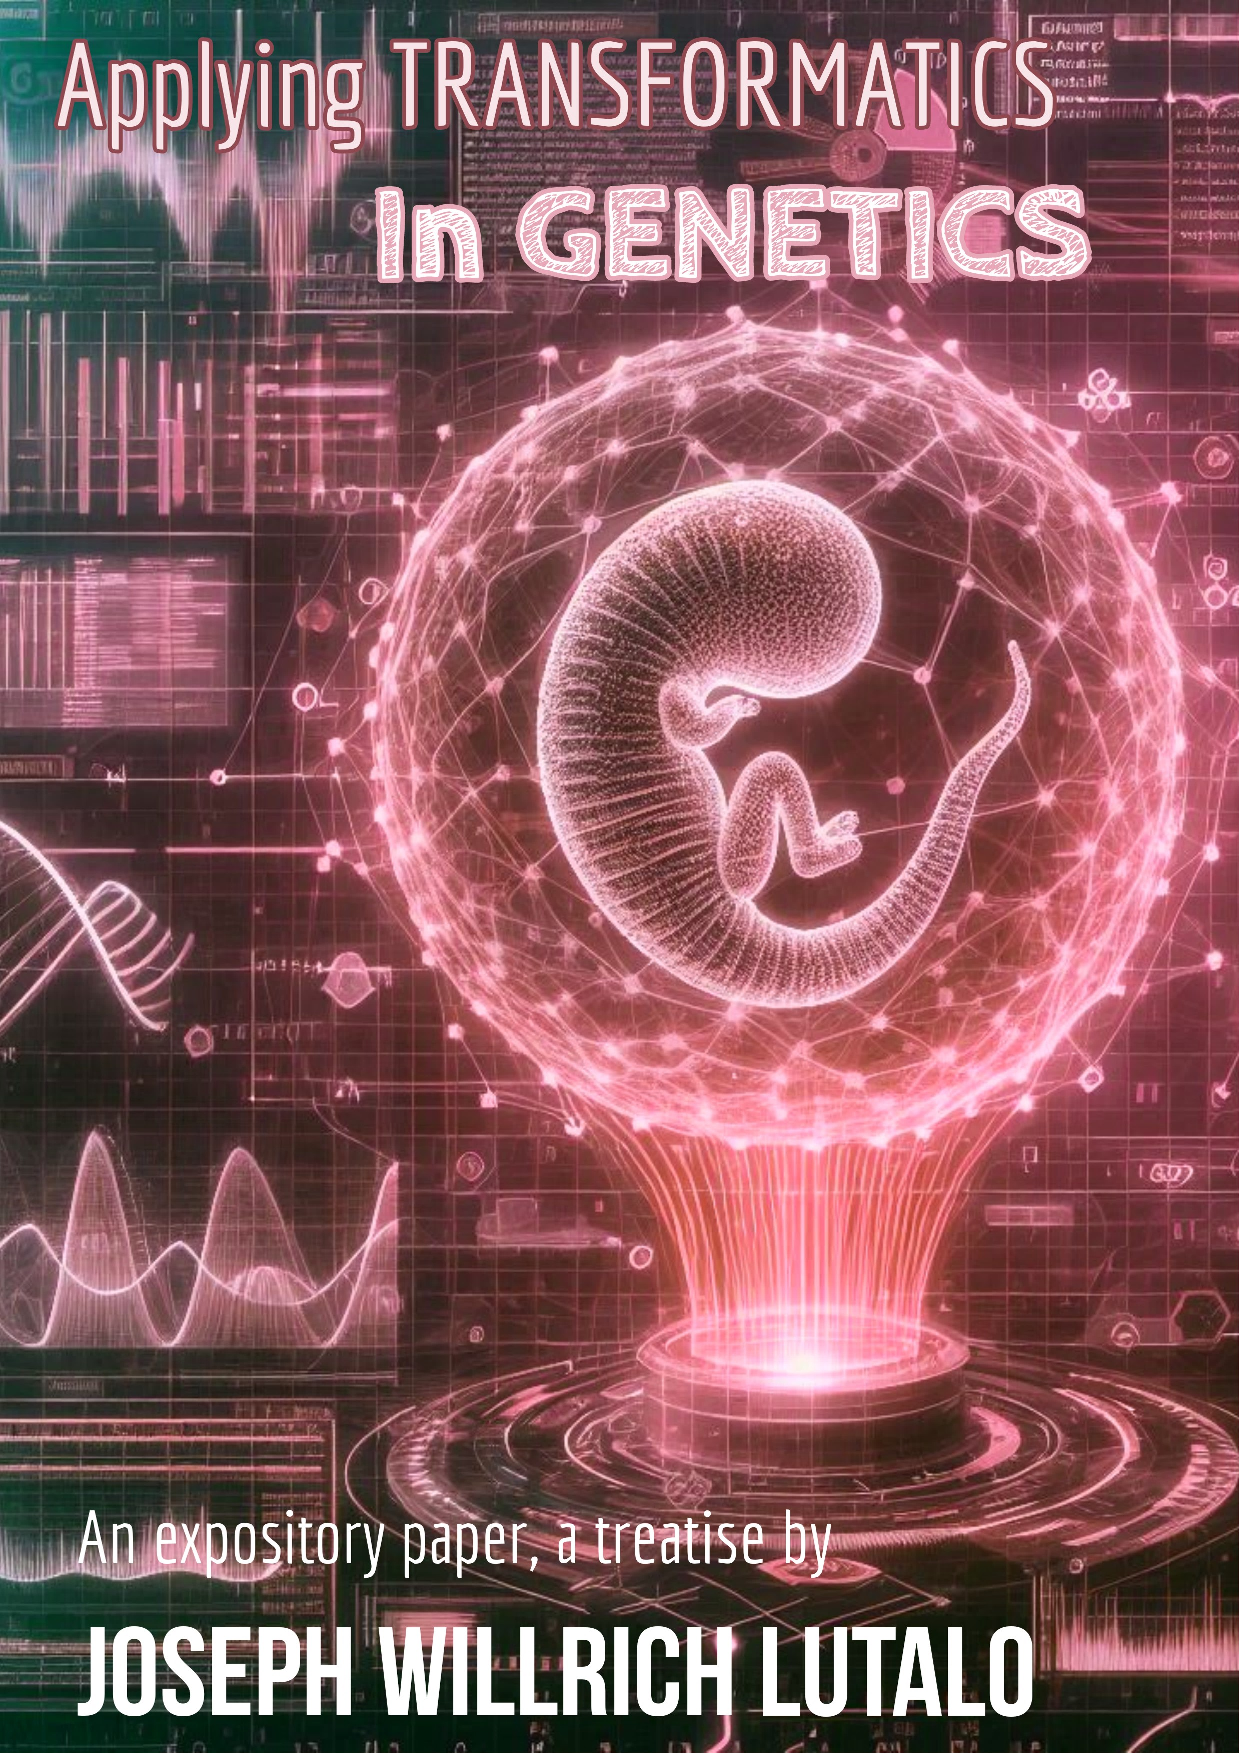
\includepdf[pages=1]{resources/pdfs/front_cover.pdf}

\maketitle


\tableofcontents

\listoffigures

\listoftables

\newpage

\Large

%\begin{abstract}
\section*{Abstract}
\large

Though still just a paper, this work brings to surface the importance of leveraging the mathematical theory recently named ``Transformatics"\cite{transformatics}, that deals with the study, processing and analysis of especially ordered sequences of symbols and their transformations. It has been demonstrated to be a credible and powerful theory in designing, specifying or explaining the properties of automata operating on sequences to produce other sequences --- so-called sequence transformers. So, in this particular work, we take that body of knowledge, as well as what we know about the critically important science of how biological life-forms get to be defined, transformed and expressed in nature via the special genetic code known as DNA (deoxyribonucleic acid), that is best modeled conceptually as an ordered sequence of genes or more technically, a sequence of special combinations of any of four chemical bases (amino acids) or just ``nucleobases" --- Adenine(A), Cytosine(C), Guanine(G), and Thymine(T), into a finite sequence typically expressed as a double-helix ladder structure, that can then be decoded by convenient biological mechanisms so as to express or rather, manufacture one or more essential life-building compounds such as proteins that underlie the synthesis of specialized aspects of the organism's body such as skin, bone and muscle tissue in an animals or into cell-wall tissue, photosynthesis machinery and others, for plant organisms. This work demonstrates how several ideas first compiled under the transformatics umbrella can be well applied in problems relating to general genetics; we for example see how to quantify how far apart or different any two organisms might be based on the anagram distance between their genetic codes, this likewise being applicable to also sub-sequences of DNA that might underlie the expression of  just particular biological machines or mechanisms. We also consider how to leverage the concept of the modal sequence statistic in analyzing not just how similar different DNA sequences might be in terms of their relative composition of the basic nucleobases, but also in terms of their relative composition at higher abstraction levels such as at the level of amino-acids or large n-gram subsequences. We finally consider the matter of how, by leveraging the idea that a modal sequence encodes a summary about some larger sequence or an entire population of them, that we can then approach DNA as though it were a special statistical summary just like the MSS from transformatics theory, and then like how complex sequences could be constructed from summary statistics via certain protraction and multiplication transformers in earlier work, we use a thought experiment to demonstrate how DNA would be transcribed into both an mRNA-like structure and then which can be further translated into actual body structures that allow the organism to occupy space and appear or behave in a particular way. Though this work is significantly theoretical and mathematical, we anticipate that these discussions and the exposition shall inspire actual domain experts and other researchers interested in genetics, genetic engineering and other sciences to pick up and apply our transformatics theory and ideas in both theory and practice.
     \newline\newline
     \textbf{Keywords}: Applied Mathematical Statistics, Transformatics, Artificial Statistical Intelligence, Information Processing, Ordered Sequences, DNA sequences, Genetic Code, Genetic Analysis, Abstract Machines
%\end{abstract}

\newpage

\section{Introduction}
\label{SEC1}


\begin{figure}[H]
  \begin{center}
  %\includegraphics[trim=2cm 8cm 2cm 8cm, clip, width=0.9\textwidth,]{resources/pdfs/ProteinSynthesisStateMachine.pdf}\\
   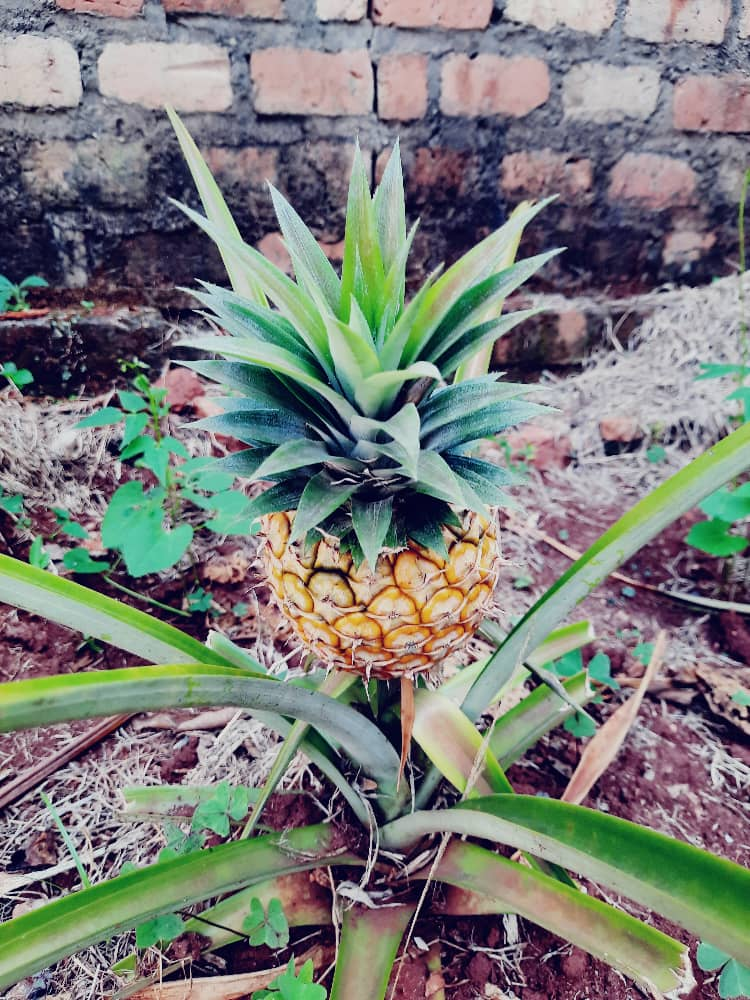
\includegraphics[width=0.9\textwidth,]{resources/images/the_pineapple.jpg}\\
   \caption{In the course of writing this work, an experiment to grow pineapples from the pineapple fruit tops of pineapples normally bought from nearby marketplace yielded results! Here we see the first successful harvest of a pineapple from our home garden. But also, this case inspired part of the discussion in \textbf{Section \ref{SEC4}} about how in real genome expression systems, the organism expressed from genetic code somewhat still includes the genetic code in the manifested organism as some kind of prefix (in leaves for example) or suffix (roots), from which the original organism can still be later reproduced!}
  \label{FIGPINEAPPLE}
  \end{center}
\end{figure}

\begin{quotation}
\noindent \texttt{Sex seems to have been invented around two billion years ago. Before then, new varieties of organisms could arise only from the accumulation of random mutations --- the selection of changes, letter by letter, in the genetic instructions. Evolution must have been agonizingly slow. With the invention of sex, two organisms could exchange whole paragraphs, pages and books of their DNA code, producing new varieties ready for the sieve of selection. Organisms are selected to engage in sex --- the ones that find it uninteresting quickly become extinct. And this is true not only for the microbes of two billion years ago. We humans have a palpable devotion to exchanging segments of DNA today.}\\
\hspace*{\fill} --- \textbf{Carl Sagan}, \textit{COSMOS}, 1981\cite{sagan1981cosmos}
\end{quotation}


\begin{quotation}
\noindent \texttt{The material basis of heredity is DNA, a ladder-like molecule which carries a message in the form of a `four-letter' code, the letters being four chemical bases, each of which may occupy any rung in the ladder.}\\
\hspace*{\fill} --- \textbf{The Oxford Companion to the Mind}\cite{gregory1987oxford}
\end{quotation}


In reality, we find that living, real organisms are influenced by genetics, their environment, bits of randomness and sometimes emergent behaviors that might not be readily captured by strict rules such as the genetic code of life. However, away from all possibilities, and focusing on what can be said of life expression via the genetic code known as DNA (the \textit{deoxyribonucleic acid}) and RNA (\textit{ribonucleic acid}), especially when applied to the vast spectrum of natural organisms on earth --- from basic \textbf{prokaryotes} (single-celled organisms) such as the simple bacteria that actually have no nucleus\cite{bioexplorer2025}, to  \textbf{eukaryotes}; all the way from basic one-cell kinds such as amoeba\cite{kang2017deep} all the way to sophisticated creatures such as oak trees, vultures, dolphins and human beings! Talking of which, it might be important to set clear that though \textbf{viruses} are a kind of life-form\cite{libretexts2025viruses}, and yet, they are neither prokaryotes nor eukaryotes --- especially because, fundamentally, they are merely some genetic code (DNA or RNA) ``enclosed in a protein coat, lacking cell membranes or organelles"\cite{libretexts2025viruses} --- more technically they are \textbf{acellular entities}.

So, if we bring on-board ideas from \textbf{transformatics}\cite{transformatics} --- a new mathematical statistics theory dealing with sequences of symbols or those of named structures and their processing as well as analysis, for example, if we take the concept of leveraging statistical measures to summarize essential properties of sequences such as DNA --- say, with use of the modal sequence statistic (MSS), we find that, independently of, and without needing to first consult or worry about mainstream genetic code analysis or genetic engineering theory and mechanics, that we can say many useful things about genetic code sequences and that we might be able to break new ground or solve some otherwise still intractable problems concerning sequences of genetic code.


\begin{figure}[H]
	\begin{center}
		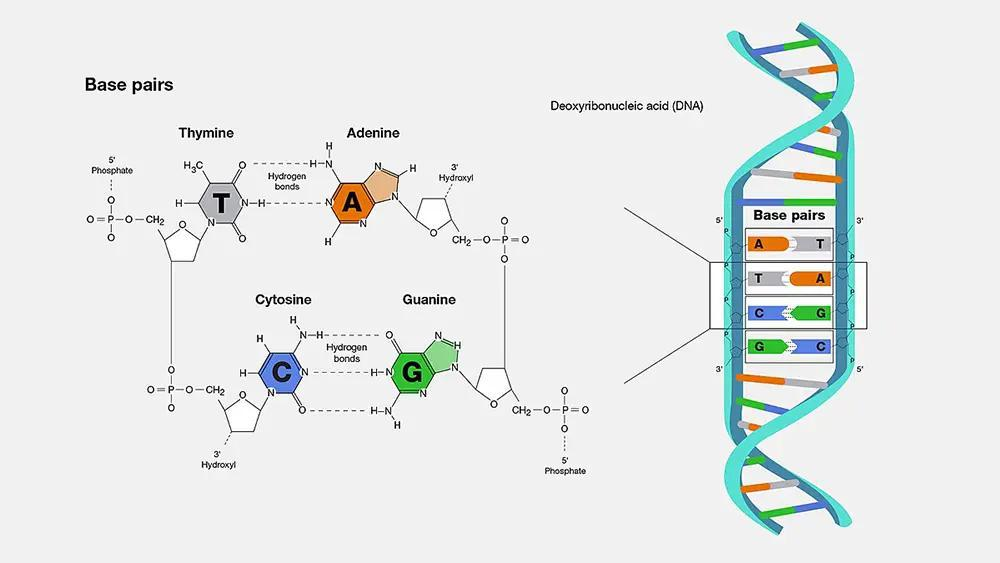
\includegraphics[width=0.9\textwidth]{resources/images/dna_diagram.jpeg} \\
		\caption{A basic diagram of the chemical structure of DNA base-pairs from \cite{wikipedia_basepair}}
		\label{FIG1}
\end{center}
\end{figure}
    


For example, by borrowing a useful DNA-as-library metaphor from Venville et al\cite{venville2006analogies}, we would come to appreciate that by looking at \textit{DNA as a library of books}, we have a model such as:

\begin{enumerate}
\item \textbf{Library}: DNA (as a whole) --- the \textbf{Genome},	 as the complete collection of genomic data about an organism.
\item \textbf{Bookshelves}: \textbf{Chromosomes} as organized storage of genes, and that they (chromosomes) are long, coiled-up strands of pairs of genes (essentially, the chromosome is a combination of two strands of genes, with one called the \textit{template} and the other a \textit{complement}, and that when they come together to form the ``ladder" structure, at each step, the two genes forming a step are paired such that $A \leftrightarrow T$ and $C \leftrightarrow G$ \cite{passel_dna_structure} --- also see \textbf{Figure \ref{FIG1}}). So, for example, humans have 46 chromosomes in total in their ``DNA library" (23 chromosome pairs, consisting of 22 autosomal pairs plus one pair of sex chromosomes). We know that during reproduction, the [full] genome (46 chromosomes in humans) splits up by half in either parent (via \textit{meiosis}, which somewhat shuffles the complete genome and then halves it\cite{genomics2025origin}), so that only one-half of the otherwise well-paired template-complement set that is the chromosome strand from each parent (as either sperm or ovum) goes to contribute to the final chromosome collection-set of the offspring\cite{libretexts2025gametogenesis}\cite{gregory1987oxford}. Whereas, after fertilization or during normal cell division, the entire chromosome set (with well-paired strands) is duplicated/replicated wholesomely and losslessly so that the second/new cell thus created has an exact copy of the same chromosome set (entire genome) as was in the source cell\cite{leicester_cellcycle}. 
\item \textbf{Books}: The \textbf{Genes} which make up a chromosome are the books in our genome library. Each gene is essentially a collection of ``words" that are a sequence of one or more codons (see below), and which taken together, contain enough information/instructions to specify how to produce a specific protein\cite{gregory1987oxford}\cite{venville2006analogies}.
\item \textbf{Words}: And then, under genes, we have \textbf{Codons} that are like ``words" in each book, and each codon \textbf{only} codes for a single \textbf{amino acid}. Basically, a codon is a combination of any 3 of the ``letters" of genetic code, for which, there are exactly four for DNA (A, C, G, T) and four for RNA (A, C, G, U). We also know that there are at most, 64 possible unique combinations of the four letters into triplets/3-grams/the codons\cite{gregory1987oxford}.
\item \textbf{Letters}: Finally, at the most basic level of our genetic code/DNA-library/genome, we have ``letters" that are technically known as \textbf{nucleotides}, and the nucleotide essentially each contains \textbf{a single nucleobase}, with only one difference between DNA and RNA as such; for DNA: $\{A, C, G, T\}$, and for RNA: $\{A, C, G, U\}$ --- we have seen the names of the four letters for DNA, and the new one for RNA, `U', stands for ``Uracil".
\end{enumerate}


So, with that introduction clearing up much of the basic genetics nomenclature and concepts that we shall use in the rest of this work, we then dive into the meat of our undertaking as such; \textbf{Section \ref{SEC2}} shall introduce the use of terminology and notation from transformatics to describe facts about genome sequences at various levels of abstraction. We shall look at using sequence symbol sets, sequence abstraction using sub-sequence symbols that can later be re-transformed into flat sequences, the idea of sequence cardinality when applied to DNA sequences and more. Then in \textbf{Section \ref{SEC3}} we shall deepen our discussion by considering how some of the measures from transformatics might be applied in genetic sequence analysis. We shall look into the ADM and PCR especially --- the other for cases where any two sequences are of the same length and similar symbol sets, and the other for cases where these need not be the same across the sequences under analysis. Then in \textbf{Section \ref{SEC4}} we shall take on the interesting matter for how, despite being merely a sequence of symbols, genetic code sequences actually can be likened to how a MSS can be used to specify how to reconstruct some other sequence. First, in \textbf{Section \ref{SEC05}} we shall first look at an overview of how actual interpretation or execution (more conventionally just referred to as ``gene translation") results in the manufacturing of proteins, and shall likewise look at some example actual gene translation in general and with a particular case. In \textbf{Section \ref{SEC5}} we shall then dive into a more hands-on exploration of this matter, with a hypothetical genome system (the \textbf{Numero-Gene Code}) that can allow us to not only creatively explore what genetic code is about, but which can also allow us to approach the rather complex matter of how DNA gets interpreted/translated into actual living tissue as well as a complete living organism. We shall introduce some two systems for how to decode our numero-gene DNA code into a kind of mRNA via the \textbf{Ozin-Transformer} and from ozin-gene code into actual tissue/proteins via the \textbf{Plato-Form Generator} that allows us to transcribe DNA into an orgnanism that has a predictable characteristic appearance and geometry, but also which still contains its essential genetic code just like normal living organisms do. Then we shall wrap-up in \textbf{Section \ref{CONC}}, looking at what we have accomplished, what remains to be done, and what the implications of this undertaking might be.

\section{Sequence Symbol Sets and Sequence Transforms Applied to Genetic Code}
\label{SEC2}

\begin{center}
\fbox{\begin{minipage}{0.9\textwidth}
\large
\textbf{NOTE:}\\
 On \textbf{Potentially Similar Mathematics}: \textit{Frobenoids?} \\

Frobenioids\cite{mochizuki_frobenioids1}, as introduced by \textbf{Prof. Shinichi Mochizuki}, offer a category-theoretic abstraction of arithmetic structures such as divisors and line bundles, encoding transformations via morphisms that resemble symbolic rewritings under algebraic constraints\cite{copilot_dna_assistant}. In spirit, they parallel the logic of sequence transformers (from transformatics\cite{transformatics}), which operate by mapping one symbolic sequence to another through rule-based transformations constrained by set-theoretic, statistical or general mathematical logic. However, even though both systems might serve as structured environments for encoding and navigating symbolic changes across mathematical objects such as sequences and/or sets, we just wanted to bring this up here, so students and researchers interested in our transformatics mathematics, and who wish to take the discussions and ideas we present in this work to even more advanced levels or in unconventional directions, pick a leaf and comfortably proceed to do so.

\end{minipage}}
\\
\end{center}

For the purposes of appreciating transformatics from a genetics engineering or general genetics research perspective, it shall be important to note that like in the original transformatics paper\cite{transformatics}, beginning by appreciating that whatever formalisms and mechanics we might develop or talk about concerning genetic code or rather DNA, had better begin with an appreciation that we can model DNA as merely an ordered sequence of symbols.\\


In the introduction (see \textbf{Section \ref{SEC1}}), we have already called out both the names and symbols assigned to the most basic units of any genetic code; essentially, the \textit{nucleobases} (or rather, nucleotides). For purposes of simplifying our mathematical logic later on, we shall here neatly define what roles these units play in the grand scheme concerning DNA and RNA code. Basically, we shall want to define the symbol sets for any DNA sequence and the symbol set for any RNA sequence.\\

\fbox{\begin{minipage}{0.9\textwidth}
\large

\begin{defn}[The \textbf{DNA Symbol Set}, $\psi_{DNA}$]
\label{DEFDNASS}

For any possible sequence of standard \textit{deoxyribonucleic acid} (\textbf{DNA}) for any possible living organism, the distinct nucleic acid base units are known as nucleotides\cite{wikipedia_nucleic_acid}, and these are essentially and exactly only four\footnote{Actually, or rather, in general, for nucleic acid sequences, the bases are four for either DNA or RNA, but, there are also conventions that extend this set to 17 or more to cater for cases like where there might be ambiguity about what the exact nucleotide in a particular position might be\cite{wikipedia_nucleic_acid}.};
\begin{itemize}
\item Adenine(A)
\item Cytosine(C)
\item Guanine(G)
\item Thymine(T)
\end{itemize}
And these are mapped to their representative, distinct single-letter symbols as shown. Thus, any possible DNA sequence must always consist of only one or more of those elements and nothing else. Thus, we might sum this up, using the symbol set concept\cite{Lutalo2024gtnc} as applied to sequences\cite{transformatics} as such:

\begin{equation}
\label{EQSSDNA}
\psi(DNA) = \{A, T, C, G\}
\end{equation}

\textbf{Equation \ref{EQSSDNA}} helps to appreciate the extra non-intuitive fact that the special ordering of DNA base symbols in the order A-T-C-G is what is conventionally accepted\cite{nature_atcg}\cite{wikipedia_nucleic_acid} or commonly found in most genetics literature\footnote{It shall be important to bring it out at this point, that, especially for non-domain experts --- people not trained in or normally practicing in genetics or related fields, that the common ordering of the nucleotides in the A-T-C-G ordering might seem unconventional or peculiar! For example, one might wonder, why are they not listed in their alphabetical order? So, for purposes of settings things clear for everyone, the author consulted a reliable research assistant on this matter\cite{copilot_dna_assistant}, and it was made clear that: ``The order **A, T, C, G** isn't alphabetical, and yet it's the most commonly used sequence when referring to DNA bases." We further learn that, the order A-T-G-C reflects a mix of historical usage and bio-chemical structure; \textbf{base-pairing logic}: that the DNA's double-helix is stabilized by ``complementary base pairing" in which A pairs with T (via 2 hydrogen bonds), and C pairs with G (via 3 hydrogen bonds), so that listing A with its partner T and then C with G emphasizes this pairing symmetry\cite{copilot_dna_assistant}. Further, we learn that early molecular biology texts and sequencing protocols (especially post-Watson \& Crick, 1953) adopted this order to reflect the ``functional relationships" between bases. It became entrenched in educational materials, sequencing software, and databases. And lastly, that in visual and structural conventions --- such as in diagrams (see \textbf{Figure \ref{FIG1}}) and models, A–T and C–G are often shown side-by-side. Listing them in this order reinforces the \textbf{duality} of the DNA ladder's rungs\cite{copilot_dna_assistant}. Lastly, that though there is no single documented moment when this convention begun, that the A-T-C-G order likely solidified in the \textbf{1970s - 1980s} during the rise of \textbf{Sanger sequencing} (developed in the 1970s), GenBank and EMBL databases, and overall in textbooks and molecular biology curricula.}.

However, and especially because, for transformatics, we wish to work with an \textbf{ordered symbol set}\cite{ossipaper} and not just \textit{any possible symbol set} so that we can apply mathematical logic that respects the ordering of terms in any ordered sequence\cite{transformatics}, we shall then assume a convention similar to how we might derive an ordered symbol set for a sequence of numbers in some base (the concept $\psi_\beta(\Theta)$ --- see \textbf{Definition 5} in \cite{ossipaper}), and given we are using Latin-Alphabet symbols (from $\psi_{az}$\cite{transformatics}) for $\psi_{DNA}$, we might as well better define the \textbf{Lexically Ordered DNA Symbol Set}, $\psi_{DNA}$ as such:

\begin{equation}
\label{EQDNASS}
\psi_{DNA} = \psi_{az}(DNA) = \langle A, C, G, T\rangle
\end{equation}

For all practical purposes unless where we merely wish to emphasize adherence to the tradition of ordering the nucleotides by their pairing order, we shall essentially imply $\psi_{az}(DNA)$ or rather $\psi_{DNA}$ when we talk of the \textbf{DNA Symbol Set}.

\end{defn}

\end{minipage}}
\\


Now that we have $\psi_{DNA}$ and $\psi_{RNA}$ well defined, we might immediately apply them to their finest use here: defining and supporting the special symbol set, $\psi_{na}$, that would or could allow for several kinds of nucleic acid sequences --- such as DNA for code stored in chromosomes and mitochondria, various kinds of RNA (\textit{m}RNA, \textit{t}RNA,...) and even synthetic/artificial/conceptual and also \textbf{random nucleic acid sequences}, etc. using a single universal nucleic acid symbol set. Thus we define $\psi_{na}$ below:


\begin{defn}[The \textit{\textbf{Universal Nucleic Acid Symbol Set}}, $\psi_{na}$]
\label{DEFUNA}
Any nucleic acid sequence, $\Theta$, obeys the following law:

\begin{law}[\textbf{Nucleic Acid Identifier Set}: $\psi_{na}$]
\label{LAWNA}
 The universal symbol set $\psi_{na}$ spans any natural nucleic acid sequence $\Theta$.
\begin{proof}
$\psi_{na} = \psi_{DNA} \cup \psi_{RNA} = \langle A, C, G, T, U \rangle$
\end{proof}
\end{law}
\end{defn}


As with many kinds of sequences dealt with in transformatics, the possession of a particular symbol set, such as $\psi_{na}$, allows for the practical use of those sets to implement logic systems that can operate on signal based on symbolic expressions of well ordered elements in sequences or sub-sequences. For this matter then, we shall likewise want to make formal, the concept of a \textbf{na-Sequence}:

\begin{defn}[The \textbf{$na-$Sequences} --- (D/R)-NA Sequences: $\Theta_{na}:\mathbb{N} \times \psi_{na}$]
\label{DEFNASEQ}

Any sequence of DNA or RNA nucleotides --- basically a sequence of nucleic acids, expressible as some sequence of symbols from $\psi_{na}$ is a \textbf{na-Sequence} and its symbol set is a superset of both $\psi_{DNA}$ and $\psi_{RNA}$. Equivalently:

\begin{equation}
\forall \Theta_{na} = \langle a_i, \rangle, \quad a_i \in \psi_{na} \implies a_i \in \psi_{DNA} \lor a_i \in \psi_{RNA}
\end{equation}

\end{defn}


If it is not immediately clear what the significance of \textbf{Defition \ref{DEFDNASS}} is or why it's important to unambiguously define $\psi_{DNA}$, then perhaps the mathematical discussions in later sections like \textbf{Section \ref{SEC3}} and \textbf{Section \ref{SEC4}} might this more obvious. That said, since we know that nucleic acid sequences come in two flavors\cite{wikipedia_nucleic_acid}, and since we have covered the essential ground for DNA symbol sets, we need now also consider the ordered RNA symbol set.\\


\fbox{\begin{minipage}{0.9\textwidth}
\large

\begin{defn}[The \textbf{RNA Symbol Set}, $\psi_{RNA}$]
\label{DEFRNASS}

For any possible sequence of standard \textit{ribonucleic acid} (\textbf{RNA}) for any possible living organism, the distinct nucleic acid base units are known as nucleotides\cite{wikipedia_nucleic_acid}, and these are essentially and exactly only four;
\begin{itemize}
\item Adenine(A)
\item Cytosine(C)
\item Guanine(G)
\item Uracil(U)
\end{itemize}
And these are mapped to their representative, distinct single-letter symbols as shown. Thus, any possible RNA sequence must always consist of only one or more of those elements and nothing else. Thus, we might sum this up, using the symbol set concept\cite{Lutalo2024gtnc} as applied to sequences\cite{transformatics} as such:

\begin{equation}
\label{EQSSRNA}
\psi(RNA) = \{A, U, C, G\}
\end{equation}

\textbf{Equation \ref{EQSSRNA}} helps to appreciate the traditional ordering of RNA base symbols in the order A-U-C-G reminiscent of the natural base-pairing order of DNA after it is translated into RNA (U merely replacing T)\cite{thoughtco_geneticcode}. And as with DNA, we shall want to have a proper, meaningful 
\textbf{ordered symbol set}\cite{ossipaper} for the RNA base symbols that we can later use in mathematical logic. Thus we shall equivalently define one for any standard RNA sequences as: 

\begin{equation}
\label{EQRNASS}
\psi_{RNA} = \psi_{az}(RNA) = \langle A, C, G, U\rangle
\end{equation}

And for all practical purposes in this work as well as after, we shall essentially imply $\psi_{az}(RNA)$ or rather $\psi_{RNA}$ when we talk of the \textbf{RNA Symbol Set} or the \textbf{Lexically Ordered RNA Symbol Set}.

\end{defn}

\end{minipage}}
\\


So, with those very essential definitions out of the way, we can begin to think of how we might appreciate and apply concepts from transformatics in genetics, in a clearer, straight forward manner.

For starters, we can certainly say that irrespective of how long or from where a particular DNA sequence, $\Theta_{DNA}$ originated from, once any sequence of data (e.g unstructured or unprocessed raw genetic code sequence dump), a string (say a proprietary encoding of some DNA code), a name (say of a particular species of interest and whose actual/representative genome sequence is know) or even a number (an id of a genome sequence in some standard genome database, etc.) is mapped to standard DNA sequence code, we shall know that any such transformation or mapping obeys \textbf{Theorem \ref{THEODNA}}:

\begin{theo}[$\psi_{DNA}$ is the alphabet of any DNA sequence]
\label{THEODNA}
For any sequence of DNA, $\Theta_{DNA}$, produced from some or any other source $\Theta$, irrespective of whether that source is itself a DNA sequence or not, we know that such an encoding or mapping, if it results in a valid DNA sequence $\Theta_{DNA}$, obeys the following general transformation:\\

\begin{trans}
\label{TRANSmDNA}
$\Theta \rightarrow \Theta_{DNA};$\\
$\forall a_{i \in [1,\invpi(\Theta_{DNA})]} \in \Theta_{DNA} \quad \exists \rho \in \psi_{DNA}: a_i = \rho$
\end{trans}

\begin{proof}
Assume $\Theta_{DNA}$ contains some symbol $\alpha$ such that $\alpha \not\in \psi_{DNA}$, it would contradict \textbf{Definition \ref{DEFDNASS}} which clearly states the legitimate membership of any DNA sequence.
\end{proof}

\end{theo}


And definitely, the equivalent truth for RNA sequences would likewise follow from \textbf{Definition \ref{DEFRNASS}}. So, we can then correctly tell that a sequence such as $\Theta_{insulin}$, which is the genetic code sequence defined as:\\


\fbox{\begin{minipage}{0.9\textwidth}
\large
%\begin{equation}
%\label{EQINSULIN}
\begin{multline}
\label{EQINSULIN}
\Theta_{insulin} =  \texttt{ATGGCCCTGTGGATGCGCCTCCTGCCCCTGCTGGCGCTGCTGGCCCTCTGGGGACC}\\
\texttt{CCAGCCGCAGCCTTTGTGAACCAACACCTGTGCGGCTCACACCTGGTGGAAGCTCTCTAC}\\
\texttt{CTAGTGTGCGGGGAACGAGGCTTCTTCTACACACCCAAGACCCGCCGGGAGGCAGAGGAC}\\
\texttt{CTGCAGGTGGGGCAGGTGGAGCTGGGCGGGGGCCCTGGTGCAGGCAGCCTGCAGCCCTTG}\\
\texttt{GCCCTGGAGGGGTCCCTGCAGAAGCGTGGCATTGTGGAACAATGCTGTACCAGCATCTGC}\\
\texttt{TCCCTCTACCAGCTGGAGAACTACTGCAACTAG}
\end{multline}
%\end{equation}
\end{minipage}}
\\

And which sequence\footnote{$\Theta_{insulin}$ is the short coding DNA sequence (CDS) for the human \textbf{INS} gene --- the part that gets transcribed into mRNA and translated by ribosomes into the insulin protein\cite{copilot_dna_assistant}}, despite having been obtained from an authority --- the \textbf{Leiden Open Variation Database (LOVD)}, which is based on NCBI's RefSeq data\cite{RefSeq}, might need to be verified by hand or with a critical eye, and that's where a law such as \textbf{Theorem \ref{THEODNA}} would come in handy. Also, note that, unlike common sequence notations we might see in this work or that we have encountered before, we wrote $\Theta_{insulin}$ in a manner somewhat more convenient for the kind of verbose sequence that DNA code generally is. The notation --- without opening or closing brackets around the sequence terms and neither commas in them might be reminiscent of the \textit{String [Chart] Sequence} notation we developed recently (see \textbf{Transformation 15} in \cite{transformatics}).

We might for example start to wonder, how might we go about determining if some two DNA sequences, $\Theta_1$ and $\Theta_2$ are the same or perhaps if they share parts of each other, and by how much? We might wonder if they are the same sequence merely shuffled/anagrammatized --- since we saw that this can occur during natural processes such as meiosis\cite{genomics2025origin}. In case they are different, we might want to for example quantify the relative frequency of their distinct members, e.g mapping $\psi_{DNA}$ or $\psi_{RNA}$ to a sequence of relative frequencies, etc. These are all things we shall soon look into and know very well how to do or talk about, using genetics terms and the mathematical language and techniques from transformatics.

\section{Sequence Abstraction using Symbol Sets: From Flat-Structure Sequences to Higher-Level Sequences}

Especially for nucleic acid sequences, but also for any other kind of sequence $\Theta$, there might be legitimate situations in which looking at or dealing with the flat-structure sequence --- such as for the actually modest\footnote{`Modest' because, genomes and realistic genome sequences can typically span millions of genes or billions of nucleotides. We for example know that for a typical human cell's DNA there are $\approx$3.2 billion base pairs\cite{Venter2001}, and yet we know each base pair consists of two nucleotides, one for each strand of the double-helix (so that's $\approx$6.4 billion), plus a few more ($\approx$16,569 base pairs) from mitochondrial DNA\cite{Anderson1981}} $\Theta_{insulin}$, might be cumbersome. And so, we are going to briefly look at ways that we might re-write verbose flat-sequences in more terse or higher-level abstract ways so as to focus on details that the flat-structure perhaps doesn't clearly express. This for example is naturally relevant in nucleic acid sequences since they are for example useful in scenarios where their processing is done in n-tuples/n-grams --- such as with codons (nucleotide 3-grams) or as gene programs (self-contained sequences of codons), etc.

So, assuming we have some sequence of symbols $\Theta_1$ defined as such:

\begin{equation}
\label{EQSEQ1}
\Theta_1 = \langle a_1, a_2,...,a_n\rangle
\end{equation}

If we wish to re-write the same sequence such that every $k$ terms are grouped in the same subsequence, we can then re-write $\Theta_1$ differently as such:


\begin{equation}
\label{EQSEQ2}
\Theta_2 = \Theta_2(n,k) = \langle a_{11}, a_{22}, a_{33}, a_{4k}, a_{51}, a_{62},...,a_{(n-k+1)(1)},...,a_{(n-k+k-1)(k-1)},a_{(n-k+k)(k)}\rangle
\end{equation}

Of course, in \textbf{Equation \ref{EQSEQ2}} we have somewhat wanted to extrapolate well and illustrate what would happen in an informative case such as when $k = 4$ and $n$ is not only significantly larger than $k$, but is also its perfect multiple. Otherwise, we might more concisely write that same sequence as:



\begin{equation}
\label{EQSEQ3}
\Theta_2(n,k) = \langle \langle a_1, a_2, a_3, a_4 \rangle_1, \langle a_5, a_6,...,a_8 \rangle_2,... , \langle a_{(n-k+1)},...,a_{(n-k+k-1)},a_{(n-k+k)}\rangle_{\frac{n}{k}} \rangle
\end{equation}

So, this expression in \textbf{Equation \ref{EQSEQ3}} is our first proper appreciation of what higher-level sequences might be like when they are an abstraction of normal flat-structure sequences. We see for example here, that the $k=4$ \textbf{bundling-parameter} means, we shall process the original flat sequence $k$ items at a time, and so, each subsequence in $\Theta_2(n,4)$ then contains exactly (or at most) 4 items --- we are assuming 4 is a factor of n to keep things simple. And so, we expect that, in total, we should have $\frac{n}{k}$ subsequences after applying the bundling transform:

\begin{transf}[The \textbf{k-GRAM Generator}]
\label{TRANSFBUND}
$\Theta = \langle a_1, a_2,...,a_n\rangle \quad \xrightarrow{O_{bundle-k}(\cdot)} \quad \Theta^* \quad;$\\
$\Theta^* = \langle \langle a_1, a_2,..., a_k \rangle_1, \langle a_{k+1},...,a_{2k} \rangle_2,... , \langle a_{(n-k+1)},...,a_{(n-k+k-1)},a_{(n-k+k)}\rangle_{\frac{n}{k}} \rangle$\\
$\forall a_i \in \Theta \quad \exists a_{ij} \in \Theta^*: a_i = a_{ij} \quad \land \quad j \in [1,k]$\\
For some $n, k \in \mathbb{N}$, and that $\invpi(\Theta^*) = \frac{n}{k} = $ number of k-gram subsequences generated from $\Theta$. $\qed$
\end{transf}


Thus, we see that the sequence depicted in \textbf{Equation \ref{EQSEQ3}} with $k=4$ could as well be produced by the generator defined in \textbf{Transformer \ref{TRANSFBUND}}. But not just that, if we applied that transformer to the DNA sequence $\Theta_{insulin}$ first presented in \textbf{Section \ref{SEC2}} --- see \textbf{Equation \ref{EQINSULIN}}, we can then produce a proper standard codon/3-gram mapping of that DNA sequence that would look something like:\\


\fbox{\begin{minipage}{0.9\textwidth}
\large
%\begin{equation}
%\label{EQINSULIN}
\begin{multline}
\label{EQINSUL2}
\Theta_{insulin} \xrightarrow{O_{bundle-3}(\cdot)}  \langle \texttt{<ATG>,<GCC>,<CTG>,<TGG>,<ATG>,<CGC>,<CTC>,...,<ACC>}\\
\texttt{...,<TAC>,<TGC>,<AAC>,<TAG>} \rangle
\end{multline}
%\end{equation}
\end{minipage}}
\\

And the way we have bundled up the nucleotides in \textbf{Equation \ref{EQINSUL2}} is exactly how a natural sequence processor such as a Ribosome (see details in \textbf{Definition \ref{DEFRIBOSOME}}) would process it so as to produce say a corresponding protein.

Of course, though we might not delve into it here or at the moment, we know that by chaining several sequence transformers --- such that one operates on the output of the previous one to produce the next sequence (see \textbf{Transformer \ref{TRANS1}} as an example), we can arrive at even higher abstraction sequences that might render certain sequence processing programs easier to write, analyze or define. For example, we know that, much as a Ribosome Processor operates on a sequence of codons, and yet, any legitimate protein synthesis and genetic code sequence processing program will require some sort of necessary delimiters (such as the START and STOP codons --- refer to the Protein Synthesis Flow Chart in \textbf{Figure \ref{FIG3}}), and so that, we might (if we could), abstract away codons and instead generate from a flat-structure DNA or perhaps mRNA sequence, a higher-level n-gram sequence of genes or \textbf{gene-program sequences}.


\section{Sequence Analysis Using Symbol Sets}
\label{SEC3}

We now turn our attention to the matter of using ideas from transformatics to help analyze or understand genetic code sequences. For starters, we shall want to consider the matter of how to tell how far apart or dissimilar any two nucleic acid sequences might be. Of course, consequently, that would also translate into meaningful way to tell how far apart not just low-level genetic-creations such as tissue, cell-types, proteins, etc might be based on the genetic code that produces them, but also how different entire organisms (within the same species or not) might be.

Because we can learn much about an organism based on its characteristic genome, and since that can be mapped to a flat-structure sequence of symbols such as we have already encountered in earlier sections, it might start to make sense to leverage the similarity/distance measures we have already developed so as to apply them to quantifying the distance between say species. In an earlier paper\cite{adtpaper}, we have introduced and also demonstrated how a sequence-analysis measure called the \textbf{Anagram Distance Measure}, $\tilde{A}(\Theta,\Theta^*)$, might be used to quantify how far apart some two sequences $\Theta$ and $\Theta^*$, that for the simplest scenarios better be of the same length, can be compared based on their common membership and the relative lexical ordering of the members in either sequence.

In the simple analysis we shall use to illustrate or develop our concepts, we shall deal with hypothetical nucleic acid sequences mostly --- especially DNA sequences, and their lengths shall be kept short to keep our analyzes simple, but also, their membership --- in terms of nucleotides, might have nothing to do with actual/natural sequences. The concepts and ideas we shall develop though, should be readily applicable to any or most nucleic acid sequences if not any sequences in general.

First, assume we have the following three sequences:

\begin{enumerate}
\item $\Theta_1 = CATGGGACTGCC$
\item $\Theta_2 = ATAATAAGAGGGATCTGA$
\item $\Theta_3 = AUAGGGAGAAUC$
\end{enumerate}

We can start by attempting to answer the question: \textbf{Which of these sequences are DNA and which are RNA?}

So, to answer that question, we can start by reducing each of those sequences to their respective [ordered] sequence symbol sets. In fact, if we first relax the assumption that they are either DNA or RNA sequences, and merely look at them as though they were any kind of sequence (for which we don't know the base or base-symbol set), then we can merely use the definition of an \textbf{Unspecific Symbol Set of $\Theta$ in Any Base} --- see \textbf{Definition 4} in \cite{ossipaper}. The algorithm for how to do that is simple and is well presented in that definition --- we basically create another sequence, in which we insert each distinct symbol from $\Theta$ that we encounter while processing the sequence from Left-to-Right\footnote{Such that the leftmost term is the first to be processed.}. Thus, we might construct the relevant transformer for this as such:

\begin{transf}[\textbf{Sequence Unspecified Symbol Set Generator}]
\label{TRANSSSGEN}$ $\\
$\Theta \xrightarrow{O_{suss-gen}(\cdot)} \Theta^* \quad;\quad \invpi(\Theta^*) \leq \invpi(\Theta) \quad \land \quad \Theta^* = \hat{\psi}(\Theta)$
\end{transf}

And thus, applying that transformer to the three sequences we have, we shall obtain the following results:

\begin{trans}
$\Theta_1 \xrightarrow{O_{suss-gen}(\cdot)} \langle C, A, T, G \rangle$
\end{trans}

\begin{trans}
$\Theta_2 \xrightarrow{O_{suss-gen}(\cdot)} \langle A, T, G, C \rangle$
\end{trans}

\begin{trans}
$\Theta_3 \xrightarrow{O_{suss-gen}(\cdot)} \langle A, U, G, C \rangle$
\end{trans}

At this juncture, we can then closely inspect the resultant sequences --- each of them a kind of symbol set, and then judge which of $\psi_{DNA}$ or $\psi_{RNA}$ they are associated with. To proceed in a rigorous manner, we might also want to compute the \textbf{Natural Symbol Set of $\Theta$ in some Base-$\beta$} --- see \textbf{Definition 5} in \cite{ossipaper}. A suitable transformer to compute such a symbol-set (for which, unlike the unspecific symbol set, orders the terms in the resultant sequence by their natural order of occurrence in the base's ordered symbol set) would as as such:\\


\begin{transf}[\textbf{Sequence $\beta$-Natural Symbol Set Generator}]
\label{TRANSNSGEN}$ $\\
$\Theta \xrightarrow{O_{snss-gen-\beta}(\cdot)} \Theta^* \quad;\quad \invpi(\Theta^*) \leq \invpi(\Theta) \quad \land \quad \Theta^* = \psi_\beta(\Theta)$
\end{transf}

And, since we already have an idea what the symbol sets for each of the three sequences are --- from which we can guess and/or disqualify some candidate bases --- e.g, since $\hat{\psi}(\Theta_3) \setminus \psi_{DNA} = \{U\}$, then $\Theta_3$ can't be a DNA sequence. However, to complete our analysis, note that:


\begin{trans}
$\Theta_1 \xrightarrow{O_{snss-gen-DNA}(\cdot)} \langle A, C, G, T \rangle$
\end{trans}

\begin{trans}
$\Theta_2 \xrightarrow{O_{suss-gen}(\cdot)} \langle A, C, G, T \rangle$
\end{trans}

\begin{trans}
$\Theta_3 \xrightarrow{O_{suss-gen}(\cdot)} \langle A, C, G, U \rangle$
\end{trans}

So, we can safely conclude that:

\begin{enumerate}
\item Since $\psi_{DNA}(\Theta_1) = \psi_{DNA}$, then $\Theta_1$ is a DNA sequence.
\item Since $\psi_{DNA}(\Theta_2) = \psi_{DNA}$, then $\Theta_2$ is a DNA sequence.
\item Since $\psi_{RNA}(\Theta_3) = \psi_{RNA}$, then $\Theta_3$ is a RNA sequence.
\item Even if we forced it, note that $\psi_{RNA}(\Theta_1) = \langle A, C, G, T \rangle \neq \psi_{RNA}$, or rather that $\hat{\psi}(\Theta_1) \setminus \psi_{RNA} = \{T\}$ so $\Theta_1$ can't be an RNA sequence.
\end{enumerate} 

Talking of which, in case we had some variation of $\Theta_1$ that has no instances of T in it, such as the sequence $\Theta_4 = CAAGGGACAGCC$, then we shall find that:

\begin{trans}
$\Theta_4 \xrightarrow{O_{suss-gen}(\cdot)} \langle C, A, G \rangle$
\end{trans}

and that:

\begin{trans}
$\Theta_4 \xrightarrow{O_{snss-gen-DNA}(\cdot)} \langle A, C, G \rangle \subset \psi_{DNA}$
\end{trans}

But also that:

\begin{trans}
$\Theta_4 \xrightarrow{O_{snss-gen-RNA}(\cdot)} \langle A, C, G \rangle \subset \psi_{RNA}$
\end{trans}

And thus, we have the peculiar case in which a nucleic acid sequence can both be a legitimate DNA or RNA sequence! However, such a truly peculiar sequence it is! Because, given the START-codon symbol set, $\psi_{na-START}$, a sequence of all the ``start" kind codons whether of DNA or RNA type, is defined as such from all we currently know:

\begin{defn}[The \textbf{Nucleic Acid START-codons}]
\label{DEFSTARTCOD}
For any known organism, prokaryote or eukaryote, the only legitimate and known codons of the START-kind are any of the codons or START 3-grams in the unordered sequence $\psi_{na-START}$, the \textbf{nucleic acid START-codon symbol set}.\\

\begin{equation}
\label{EQNNASSS}
\psi_{na-START} = \{ATG,AUG,GTG,GUG,TTG,UUG\}
\end{equation}\\

So, that, if say a nucleic acid program for producing some protein via some gene program $\Theta_{na}$ were to be processed by an ideal ribosome (see \textbf{Definition \ref{DEFRIBOSOME}}), the ribosome would never produce anything --- or, equivalently, there is no guarantee that any protein would be produced no matter what or any instructions the gene program contains, as long as it doesn't contain any one of the members of $\psi_{na-START}$.
\end{defn} 

One interesting consequence of that definition is the following law:

\begin{law}[\textbf{Non-Coding Gene Programs\footnote{Also known as \textbf{Introns} in some contexts.}}]
If any gene-program $\Theta_{na}$ is processed by a ribosome, and yet it has the property:\\

 $\psi_{DNA}(\Theta_na) \cap \psi_{na-START} = \emptyset \quad \lor \quad \psi_{RNA}(\Theta_na) \cap \psi_{na-START} = \emptyset$\\
 
It implies that $\Theta_{na}$ shall never be transcribed by the ribosome, and neither shall it ever result in any new protein or new amino-acid product within the containing cell system\footnote{Refer to ribosome definition for details: \textbf{Definition \ref{DEFRIBOSOME}}}.
\end{law}


So, that, if say a nucleic acid program for producing some protein via some gene program $\Theta_{na}$ were to be processed by an ideal ribosome processor (see \textbf{Definition \ref{DEFRIBOSOME}}), the ribosome would never return --- or, equivalently, there is no guarantee that any products --- neither amino-acid, nor completed/new protein, shall be synthesized by the ribosome.

Of course, it's very likely that such gene sequences exist, and there might be nothing wrong with them being natural too. However, we shall want to learn more about this from the domain experts in the future.

That said, another, closely related case is that of the consequences of the STOP-codons or rather, the STOP-codon symbol set, $\psi_{na-STOP}$ defined as such:


\begin{defn}[The \textbf{Nucleic Acid STOP-codons}]
\label{DEFSTOPCOD}
For any known organism, prokaryote or eukaryote, the only legitimate and known codons of the STOP-kind are any of the codons or STOP 3-grams in the unordered sequence $\psi_{na-STOP}$, the \textbf{nucleic acid STOP-codon symbol set}.\\

\begin{equation}
\label{EQNNASSSTOP}
\psi_{na-STOP} = \{TAA,UAA,TAG,UAG,TGA,UGA\}
\end{equation}\\
\end{defn} 

Among important consequences of \textbf{Definition \ref{DEFSTOPCOD}}, is that, if say a nucleic acid program for producing some protein via some gene program $\Theta_{na}$ were to ever be processed by an ideal ribosome (see \textbf{Definition \ref{DEFRIBOSOME}}), the ribosome might produce something --- some amino-acids for example, but would never return --- equivalently, there is no guarantee that any protein would be released by the protein manufacturing process/ribosome, no matter what or how many any amino-acid productions and translate instructions the gene program contains and which have been executed by the ribosome. As long as the gene-program doesn't contain any one of the members of $\psi_{na-STOP}$ that is.

It is not immediately clear what the plausibility of such an \textit{evil gene-program} existing out there in nature might be, but given normal genes sometimes mutate\cite{gregory1987oxford}, it can't be ruled out that such awkward programs might exist. Though we won't dive into that here, who knows... from a computer security perspective, such a program might cause system errors or faults such as a System-Out-Of-Resources problem given the ribosome might attempt to produce an infinite length amino-acid, or perhaps that the cell's protein manufacturing closure might run out of space, or that the processor might end up hanging since the factory never is able to reach any of WAIT, DETACH or RESET states --- see \textbf{The Ribosome State Machine} in \textbf{Figure \ref{FIG4}} but also refer to the Protein Synthesis Process in \textbf{Figure \ref{FIG3}} to clearly, logically appreciate these kinds of problems and/or corner-case scenarios. 

That said, in case a normally correct gene-program such as what we saw in $\psi_{insulin}$ (see \textbf{Equation \ref{EQINSULIN}}) is altered with --- perhaps by a natural mutation, or perhaps a virus, or even in a totally malicious feat of gene-manipulation medicine, and such a transformation results in a nucleic-acid sequence satisfying any of the above queer cases, who knows, but it might as well be the root case of some difficult flaw in the organism --- an incurable and fatal disease (if the faulty gene-program is crucial for normal life support and that it has no alternatives or simple way to be solved), and these might the kinds of hard problems that might require not just medical doctors, biologists or perhaps genetists to tackle, but also people like computer hackers, information-security experts and software debuggers\footnote{It shouldn't come as a surprise, that with a stronger marriage of computing theory and biology, or medicine, that certain problems in nature --- not just with humans or animals, but also with plants for example, and especially if they are either inheritable --- meaning genetic, or if they might somehow be remedied via clever hacking or debugging and modifying of the organism via gene programs, might call for the skills of and expertise of software engineers and program debuggers from hardcore computer science and not just the medical or biological sciences! A great background work on this subject by the author might come in handy --- refer to \cite{Lutalo2025debug}}!

\section{Sequence Analysis Using Complement Sets}
\label{SEC3A}

The idea of complements when applied to na-Sequences has already been introduced in \textbf{Section \ref{SEC1}}, and we get to see it depicted in an exemplary typical diagrammatic depiction of the DNA structure in \textbf{Figure \ref{FIG1}}. However, apart from having talked about the fact that nucleic acids typically or naturally occur together in base-pairs depicting pairwise complements, we might want to leverage transformatics to study this idea at a more general level --- say, to explore the matter of \textbf{na-Sequence} (as well as \textit{any sequence}) complements, and thus this section.

Assume we start by exploring simple binary sequences --- especially because bits help generalize many ideas in theory and practice. We can for example start by noticing that, like in the case of the interesting \textbf{Lu-Number System}\cite{lnspaper} --- in which any kind of \textit{basic information} can be abstracted by mapping it to either signal (>) or anti-signal (<), and that \textit{complex information} can then be generated from that using transforms on basic LNS sequences or expressions, etc. We can start by looking at what can be said of the transforms on the binary sequence symbol set, $\psi_{bin}$ --- or better, $\psi_{01}$. In our formulations, we shall denote the complement of a symbol $\rho$ by $\lnot\rho$, and for a sequence $\Theta$, with $\lnot\Theta$.


\begin{table}[H]
  \centering
  \Large
	\begin{tabular}[t]{|p{2cm}|c|c|p{4cm}|}
	\hline
	Sequence Name & Sequence & Formula & Note\\
	\hline
	\hline
	$\Theta1$ & 0 1 & $\psi_{01}$ & Binary Symbol Set as a basic Sequence\\
	\hline
	$\Theta2$ & 0 1 0 1 & $\psi_{01}\cdot\psi_{01}$ & Sequence Concatenation/Multiplication\\
	\hline
	$\Theta3$ & 0 2 0 1 & $\psi_{01}(1 + \psi_{01})$ & Sequence as Linear Combination of other Sequences: case of memberwise addition of the above two sequences\\
	\hline
	$\Theta4$ & 1 0 1 0 & $\lnot\Theta2 = \lnot\psi_{01} \cdot \lnot\psi_{01}$ & Basic Complement Transforms\\
	\hline
	              
\end{tabular}
 \caption{An example of exploring symbol and sequence complements in sequence transformations}
  \label{TABCOMPLEMENTS}
\end{table}

So, we can begin by noting that, if some sequence $\Theta$ spans some symbol set $\psi_\beta$ --- such as how all the sequences in \textbf{Table \ref{TABCOMPLEMENTS}} span $\psi_{01}$, then we can say that the complement sequence, $\lnot\Theta$ spans the complement symbol set $\lnot\psi_\beta$. But not just that. You can readily tell from studying that table, that actually, if sequence $\Theta$ spans $\psi_\beta$, then it also spans $\lnot\psi_\beta$ --- meaning, its members essentially are one of the distinct elements from either symbol set even though the two sets might not necessarily have the same ordering of their members.

Further, note that, if $\psi_\beta$ is the symbol set of some sequence $\Theta$, and that the \textbf{complement symbol set} it is equivalent to is $\lnot\psi_\beta$, then we can comfortably say that $\lnot\Theta$ spans $\lnot\psi_\beta$ as well. This is true, because, for any sequence $\Theta$, its complement, $\lnot\Theta$ is the sequence of the memberwise complements of $\Theta$. That is to say:

\begin{equation}
\psi_\beta = \lnot (\lnot \psi_\beta)
\end{equation}

and 

\begin{equation}
\Theta = \lnot(\lnot\Theta) \implies \lnot\Theta = \lnot(\Theta)
\end{equation}

So that, if

\begin{equation}
\label{EQCOMPSETS}
\psi_\beta = \langle \prod\limits_{i=1}^{n} a_i \rangle \quad \implies \quad \lnot\psi_\beta = \langle \prod\limits_{i=1}^{n} a_{n-i} \rangle
\end{equation}

And for any $\Theta: \mathbb{N} \times \psi_\beta$ we know that:

\begin{equation}
\lnot\Theta = \prod\limits_{i=1}^{n} \lnot(a_i)
\end{equation}

for $n = \invpi(\Theta)$ and that $\forall a_i \in \psi_\beta$, 

\begin{equation}
\label{EQCOMPLEMENTS}
\lnot(a_i) = \rho_i \in \lnot\psi_\beta
\end{equation}


So, one way to appreciate \textbf{Equation \ref{EQCOMPLEMENTS}}, is by realizing that by knowing the members and their order in $\psi_\beta$, we can then systematically determine the members and ordering of $\lnot\psi_\beta$ via \textbf{Equation \ref{EQCOMPSETS}}, and so that, for some $a_i$ in $\psi_\beta$, its complement in $\lnot\psi_\beta$ is the term at position index $n-1$ in $\psi_\beta$. Thus, as we saw in \textbf{Table \ref{TABCOMPLEMENTS}}, for $a_0 = 0$ in $\psi_{01}$, the complement, $\lnot a_0 = a_{\invpi(\psi_{01})-0} = a_2 = 1$. This mechanics can be extended or applied to sequences of arbitrary length and composition as necessary. For purposes of future use, we shall generalize this with a useful theorem as such:


%\fbox{\begin{minipage}{0.9\textwidth}
%\large

\begin{theo}[\textbf{Complement Sequences}]
\label{THEOCOMPLEMENTS}

For any ordered sequence $\Theta_n\langle \prod\limits_{i=1}^{n} a_i \rangle$, its equivalent \textbf{complement sequence}, also denoted $\lnot\Theta_n$, is the sequence with the signature $\Omega_n\langle \prod\limits_{i=1}^{n} \rho_i \rangle$ such that $\rho_i = a_{n-1} \quad \forall a_i \in \Theta_n$. We shall also write $\Omega_n$ as $\lnot\Theta_n$ where necessary.

\begin{proof}
By \textbf{Equation \ref{EQCOMPSETS}}, we see that if $\Theta_n = \langle a_1, a_2, a_3,...,a_{n-1}, a_n \rangle$, then we can derive its complement $\lnot\Theta_n$ via the mapping of its members to corresponding members in its lateral inverse as such:

\[
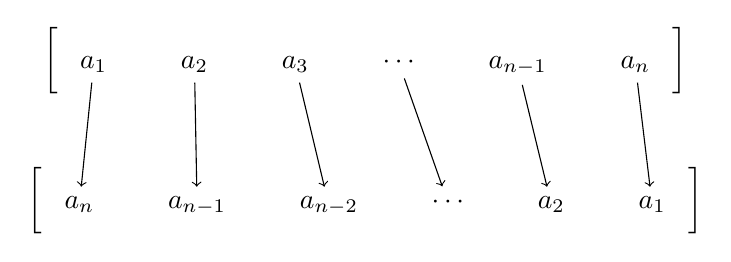
\begin{tikzpicture}[baseline=(current bounding box.center)]
  % Matrix A
  \matrix (A) [matrix of math nodes, left delimiter={[}, right delimiter={]}, row sep=1em, column sep=2em] {
    a_1 & a_2 & a_3 & \cdots & a_{n-1} & a_n \\
  };

  % Matrix B
  \matrix (B) [matrix of math nodes, left delimiter={[}, right delimiter={]}, row sep=1em, column sep=2em, below=3em of A] {
    a_n & a_{n-1} & a_{n-2} & \cdots & a_2 & a_1 \\
  };

  % Draw arrows from A_i to B_i
  \foreach \i in {1,2,3}
    \draw[->] (A-1-\i) -- (B-1-\i);

  % Optional: arrows for ellipsis and final element
  \draw[->] (A-1-4) -- (B-1-4); % for \cdots
  \draw[->] (A-1-5) -- (B-1-5); % for a_{n-1} → b_{n-1}
  \draw[->] (A-1-6) -- (B-1-6); % for a_n → b_n
\end{tikzpicture}
\]

\end{proof}

\end{theo}
%\end{minipage}}
%\\

And since we are dealing with sequence transformations in this work, we might as well define the necessary transformer:

\begin{transf}[The \textbf{Complement Transformer}]
\label{TRANSCOMPL}
$ $\\
$\Theta \xrightarrow{O_{complement}(\Theta)} \Theta^*; \quad \Theta^* = \lnot\Theta$
\end{transf}


\subsection{Significance of Sequence Complements, $\lnot\Theta$ and Complement Symbol Sets, $\lnot\psi_\beta$}

First, we shall momentarily return to binary sequences. 

We note that, for some binary sequence $\Theta: \mathbb{N} \times \psi_{01}$, the transform

\begin{trans}
$\Theta \xrightarrow{O_{complement}(\cdot)} \Theta^*; \Theta^* = \lnot\Theta$
\end{trans}

which applies \textbf{Transformer \ref{TRANSCOMPL}}, produces the same sequence as $\Theta$ but with all bits swapped by their complements, which, as per usual nomenclature in computer science for example, means the resultant sequence is produced from the source via a \textbf{bitwise NOT operation}, and which, for binary sequences, is as simple as merely flipping the bits individually.

Thus, if our source sequence was 

\begin{equation}
\Theta = \langle 0 1 0 1 1 1 1 0 \rangle
\end{equation}

Then 

\begin{trans}
$\Theta \xrightarrow{O_{complement}(\Theta)}  \langle 1 0 1 0 0 0 0 1 \rangle$
\end{trans}

And then, returning to nucleic acid sequences, we note that if we for example have some na-Sequence such as 

\begin{equation}
\label{SEQATC}
\Theta = \langle A T C G C G T A T \rangle
\end{equation}

\textbf{That we wish to treat as a DNA-sequence}, then its \textit{na-Complement} sequence would be derivable from $\psi_{DNA}$ as such:

Since $\psi_{DNA} = \langle A, C, G, T \rangle$, then by \textbf{Equation \ref{EQCOMPSETS}}, we know that:

\begin{equation}
\lnot(\psi_{DNA}) = \lnot\psi_{DNA}) = \langle T, G, C, A \rangle
\end{equation}

So that, $\forall \rho \in \psi_{DNA}$, the equivalent complement is via the mapping:

\[
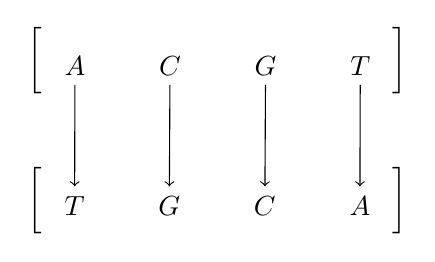
\begin{tikzpicture}[baseline=(current bounding box.center)]
  % Matrix A
  \matrix (A) [matrix of math nodes, left delimiter={[}, right delimiter={]}, row sep=1em, column sep=2em] {
    A & C & G & T \\
  };

  % Matrix B
  \matrix (B) [matrix of math nodes, left delimiter={[}, right delimiter={]}, row sep=1em, column sep=2em, below=3em of A] {
    T & G & C & A \\
  };

  % Draw arrows from A_i to B_i
  \foreach \i in {1,2,3, 4}
    \draw[->] (A-1-\i) -- (B-1-\i);
\end{tikzpicture}
\]

Which is also the consequence of \textbf{Theorem \ref{THEOCOMPLEMENTS}}. Thus, for the sequence in \textbf{Equation \ref{SEQATC}}, the corresponding complement DNA sequence is:

\begin{equation}
\label{SEQATCCOMP}
\lnot\Theta = \langle T A G C G C A T A \rangle
\end{equation}

This ideal can be further appreciated by noticing that the traditional DNA sequence base symbol set (which we shall denote by $\dot{\psi}_{DNA}$), is actually different from $\psi_{DNA}$, and is defined as:

\begin{equation}
\label{SSDNAT}
\dot{\psi}_{DNA} = \langle A, T, C, G \rangle
\end{equation}

We should come to appreciate this special symbol set, or even justify it --- for logical and mathematical analyses, by acknowledging that it depicts not just a sequence of distinct symbols from $\psi_{DNA}$, but also their natural order based on both order of occurrence in $\psi_{DNA}$ \textbf{and} their equivalent \textbf{symbol complements} in $\lnot\psi_{DNA}$! It is such a terrific discovery/realization. And before we proceed, we note that the $\dot{\psi}_{DNA} \rightarrow \lnot\dot{\psi}_{DNA}$ mapping for pairwise-ordered DNA sequences is as such:


\[
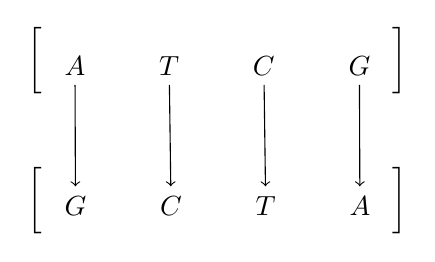
\begin{tikzpicture}[baseline=(current bounding box.center)]
  % Matrix A
  \matrix (A) [matrix of math nodes, left delimiter={[}, right delimiter={]}, row sep=1em, column sep=2em] {
    A & T & C & G \\
  };

  % Matrix B
  \matrix (B) [matrix of math nodes, left delimiter={[}, right delimiter={]}, row sep=1em, column sep=2em, below=3em of A] {
    G & C & T & A \\
  };

  % Draw arrows from A_i to B_i
  \foreach \i in {1,2,3, 4}
    \draw[->] (A-1-\i) -- (B-1-\i);
\end{tikzpicture}
\]


Because, from \textbf{Equation \ref{SSDNAT}}, we can tell that:

\begin{equation}
\label{SSDNATCOMP}
\lnot\dot{\psi}_{DNA} = \langle G, C, T, A \rangle
\end{equation}


Perhaps, and worth checking out, even if momentarily, what would happen when the idea of complement symbols sets and complement sequences is applied to the more commonplace base-10 sequences (aka ``usual numbers")?

First, note that since $\psi_{10}$ --- our choice of symbol for the decimal symbol set, is expressed as such:

\begin{equation}
\label{SSDEC}
\psi_{10}= \langle 0, 1, 2, 3, 4, 5, 6, 7, 8, 9 \rangle
\end{equation}

Then, by \textbf{Theorem \ref{THEOCOMPLEMENTS}}, its complement is:


\begin{equation}
\label{SSDEC}
\lnot\psi_{10}= \langle 9, 8, 7, 6, 5, 4, 3, 2, 1, 0 \rangle
\end{equation}

So that, for any base-10 digit, the corresponding \textbf{complement digit} is as in the mapping below:


\[
\begin{tikzpicture}[baseline=(current bounding box.center)]
  % Matrix A
  \matrix (A) [matrix of math nodes, left delimiter={[}, right delimiter={]}, row sep=1em, column sep=2em] {
    0 & 1 & 2 & 3 & 4 & 5 & 6 & 7 & 8 & 9\\
  };

  % Matrix B
  \matrix (B) [matrix of math nodes, left delimiter={[}, right delimiter={]}, row sep=1em, column sep=2em, below=3em of A] {
    9 & 8 & 7 & 6 & 5 & 4 & 3 & 2 & 1 & 0\\
  };

  % Draw arrows from A_i to B_i
  \foreach \i in {1,2,3,4,5,6,7,8,9,10}
    \draw[->] (A-1-\i) -- (B-1-\i);
\end{tikzpicture}
\]

Such a peculiar cipher! Because, usual/familiar number sequences such as the \textbf{Hi-Fi o-SSI}\cite{adtpaper}, defined as such:

\begin{equation}
\Theta_{HiFi} = 8 6 4 9 1 3 7 5 2 0
\end{equation}

Has the complement:


\begin{equation}
\lnot\Theta_{HiFi} = 1 3 5 0 8 6 2 4 7 9
\end{equation}

Which, given how that special sequence was derived/discovered(see \textbf{Section 5.1} in \cite{ossipaper} or \textbf{Equation 19} in the same paper), it is interesting to note that its complement under $\psi_{10}$ is also an \textit{orthogonal symbol set identity}! For those who have studied the o-SSI paper\cite{ossipaper}, this can really be exciting for the study of symbol sets and sequences in general --- yes, even for nucleic acid sequences! But, that said, of course, it shouldn't come as a surprise, since, in simple terms, a sequence's complement is just one very special kind anagram among the set of all potential anagrams it can have, and so, before we leave the base-10 case, we can note that if some sequence $\Theta_{10}: \mathbb{N} \times \psi_{10}$ is a base-10 o-SSI, then its complement is also a base-10 o-SSI, and in fact, in general --- even for non-numeric symbol sets such as $\psi_{na}, \psi_{DNA}$ or special $\psi_{RNA}$, that:


\begin{theo}[\textbf{Complement of an o-SSI is an o-SSI}]
If some sequence $\Theta: \mathbb{N} \times \psi_\beta$ is an orthogonal symbol set identity for the base $\beta$, then its complement, $\lnot\Theta$ is also an orthogonal symbol set identity for $\beta$.
\end{theo}

\subsection{Potential Applications of Sequence Complements or Inverses}
\label{SECAPPCOMPLEMENTS}

First, in genetics and analysis of genetic code sequences, note that for especially sequences in say the \textit{non-native}(non-storage) form, such as the processed/derived RNA-sequences, it might sometimes be useful to determine if some two sequences are the same, equivalent or closely related, even though their apparent ordering of members, or even member composition looks unlike, \textbf{as long as their cardinalities are the same}\footnote{This requirement to have their sizes the same, is a natural consequence of how a sequence and its anagram relate --- see \cite{adtpaper}}.

We should note, and interestingly so, that the complement of any sequence $\Theta$, which is $\lnot\Theta$, is just an anagram of $\Theta$, and that in general, we can comfortably say:


\begin{theo}[\textbf{Equivalence of Sequences under the Complement Transform}]
If two sequences $\Theta$ and $\Omega$ that are \textbf{not equal}, but which do have the same cardinality and similar distribution of members, then they are essentially equivalent under the sequence complement transform.

\begin{proof}
The proofs are several:
\begin{enumerate}
\item Since $\invpi(\Theta) = \invpi(\Omega)$ and $\forall \alpha \in \Theta \quad \exists \rho \in \Omega: \alpha = \rho$ or equivalently, that $\forall a_i \in \Theta, \invpi(a_i \in \Theta) = \invpi(a_i \in \Omega)$, then there exists some anagram of $\Theta$, denoted $\Theta^*$ such that $\Theta^* \xrightarrow{O_{complement}(\cdot)} \Omega$, which is possible by \textbf{Theorem \ref{THEOCOMPLEMENTS}}.
\item Because sequence complements are anagrams of each other, then if the two sequences are complements of each other, we expect that by the definition of the complement transformer (see \textbf{Transformer \ref{TRANSCOMPL}}), $\Omega = \lnot\Theta$ or that $\Theta = \lnot\Omega$.
\item We might also proceed by use of \textbf{modal sequences}(see \textbf{Definition 1} in \cite{transformatics}): Given the conditions on the two sequences, we then expect that if $\Theta$ is a sequence complement of $\Omega$ or vice-versa, then, computing their corresponding modal sequence statistic should result in the following result: $\overset{>}{\Theta} = \lnot(\overset{>}{\lnot\Omega})$ or equivalently, $\overset{>}{\Omega} = \lnot(\overset{>}{\lnot\Theta})$
\end{enumerate}
\end{proof}

\end{theo}


Note that, for RNA, since $\psi_{RNA} = \langle A, C, G, U \rangle$ (\textbf{Equation \ref{EQRNASS}}), then: 

\begin{equation}
\label{EQRNACOMP}
\lnot\psi_{RNA} = \langle U, G, C, A \rangle
\end{equation}

And this is what we'd expect via the complement mapping:


\[
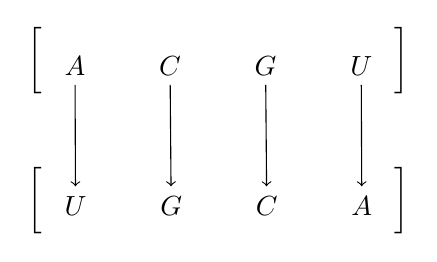
\begin{tikzpicture}[baseline=(current bounding box.center)]
  % Matrix A
  \matrix (A) [matrix of math nodes, left delimiter={[}, right delimiter={]}, row sep=1em, column sep=2em] {
    A & C & G & U \\
  };

  % Matrix B
  \matrix (B) [matrix of math nodes, left delimiter={[}, right delimiter={]}, row sep=1em, column sep=2em, below=3em of A] {
    U & G & C & A \\
  };

  % Draw arrows from A_i to B_i
  \foreach \i in {1,2,3, 4}
    \draw[->] (A-1-\i) -- (B-1-\i);
\end{tikzpicture}
\]


But, since the traditional pairwise ordered symbol set for RNA, $\dot{\psi}_{RNA}$ is


\begin{equation}
\label{EQRNATRAD}
\dot{\psi}_{RNA} = \langle A, U, C, G \rangle
\end{equation}

Then its corresponding complement,$\lnot\dot{\psi}_{RNA}$, is

\begin{equation}
\label{EQRNATRADCOMP}
\lnot\dot{\psi}_{RNA} = \langle G, C, U, A \rangle
\end{equation}

And so we have the associated complement mapping as

\[
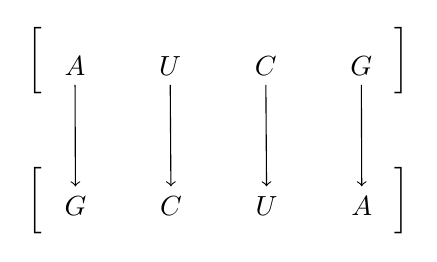
\begin{tikzpicture}[baseline=(current bounding box.center)]
  % Matrix A
  \matrix (A) [matrix of math nodes, left delimiter={[}, right delimiter={]}, row sep=1em, column sep=2em] {
    A & U & C & G \\
  };

  % Matrix B
  \matrix (B) [matrix of math nodes, left delimiter={[}, right delimiter={]}, row sep=1em, column sep=2em, below=3em of A] {
    G & C & U & A \\
  };

  % Draw arrows from A_i to B_i
  \foreach \i in {1,2,3, 4}
    \draw[->] (A-1-\i) -- (B-1-\i);
\end{tikzpicture}
\]


So, that, for some RNA-sequence such as $\Theta_{met}$:


\begin{equation}
\Theta_{met} = \langle A, U, G \rangle
\end{equation}


Which is the famous START-codon \textbf{Methionine} (see \textbf{Table \ref{TAB2}}), has as its corresponding nucleic acid sequence complement under $\dot{\psi}_{RNA}$:

\begin{trans}
\label{TRANSGCA}
$\Theta_{met} \xrightarrow{O_{complement}(\Theta,\dot{\psi}_{RNA})}  \langle G, C, A \rangle$\\
That codon isn't the same as the source (ATG/AUG/Methionine), but there's some debate concerning what it actually is called --- \textbf{Table 1} in \cite{gregory1987oxford} names codon GCA as \textbf{Arginine}, while Wikipedia\cite{wikipedia_codon_tables} names it \textbf{Alanine}.
\end{trans}

While --- \textbf{and important to note}, its complement under $\psi_{RNA}$ is [indeed] different!

\begin{trans}
\label{TRANSUAC}
$\Theta_{met} \xrightarrow{O_{complement}(\Theta,\psi_{RNA})}  \langle U, A, C \rangle$
\\
and we know that codon UAC is Tyrosine\cite{wikipedia_codon_tables}\footnote{Concerning this particular codon, TAC/UAC, we find that though the Wikipedia reference tables assign it the name Tyrosine in both the DNA and RNA encodings, and yet, the physical reference we have at hand\cite{gregory1987oxford} (perhaps now out-of-date), assigns the name ``Methionine" to TAC --- Table 1 in that reference book didn't list RNA codes, but we still would expect to use TAC to look-up the correct name for UAC.}.
\end{trans}

It should perhaps be immediately noticeable that the ability to derive new/different/special sequences such as complement codons from ordinary na-Sequences might have some useful if not exciting applications as well as problems it awakens for the geneticists, molecular biologists and researchers of gene-sequencing\footnote{For those that don't know: Gene sequencing is the process of determining the exact order of nucleotides --- A, T, C and G --- in a segment of DNA that makes up a gene. It's like reading the biological ``code" that instructs cells how to build proteins and regulate functions\cite{copilot_dna_assistant}.} and analysis. For example, apart from acknowledging that na-Sequence's complements denote potentially legitimate na-helix strand partners for any two sequences (in the form $\Theta$ and $\lnot\Theta$), it would be interesting to determine what other important things might we learn, discover from exploring these kinds of sequence transforms? 

It's already interesting to note that under complement transforms (which are special kinds of anagrams), the natural/universal protein synthesis START-codon AUG/ATG is equivalent to GCA (\textbf{Transformation \ref{TRANSGCA}}) or UAC (\textbf{Transformation \ref{TRANSUAC}}), but, \textbf{are those other codons also START-codons?} That said, is there a possibility that some natural process or genetic code translation or transformation might naturally produce ATG or AUG from any of those corresponding [symbolic] complement sequences? What would this teach us about natural/biological processors? What of the possibilities of using synthetic/artificial processors to render such complement operations useful?


\section{Sequence Analysis Using The Anagram Distance and the Modal Sequence Statistic}
\label{SEC4A}


We are going to talk about the matter of comparing or analyzing two or more na-Sequences using especially statistical measures that have been set down by transformatics theory for especially ordered sequences. 

\subsection{Six Sequences and Four Scenarios}
\label{SEC4ASEQ}

In particular, we shall be looking at na-Sequence analysis through lens of measures we have formalized earlier on, and shall break down our analysis into four representative scenarios:

\begin{enumerate}
\item \textbf{Scenario A:} Given some two particular instances of na-Sequences, $\Theta1_n$ and $\Theta2_n$, of the same length, $n$, and with similar symbol sets ($\psi_{na}(\Theta1_n) = \psi_{na}(\Theta2_n)$), how to quantify how similar or dissimilar they are?
\item \textbf{Scenario B:} Given some two particular instances of na-Sequences, $\Theta1_n$ and $\Theta2_k$, of different lengths, $n$ and $k$, but with similar symbol sets ($\psi_{na}(\Theta1_n) = \psi_{na}(\Theta2_k)$), how to quantify how similar or dissimilar they are?
\item \textbf{Scenario C:} Given some two particular instances of na-Sequences, $\Theta1_n$ and $\Theta2_k$, of different lengths, $n$ and $k$ and with different symbol sets ($\psi_{na}(\Theta1_n) \neq \psi_{na}(\Theta2_k)$), how to quantify how similar or dissimilar they are?
\item \textbf{Scenario D:} Finally, how, when given a particular na-Sequence, $Q_k$, and two collections/samples of other sequences ($\Theta1, \Theta2, \Theta3,..., \Theta m$) and ($\Omega1, \Omega2, \Omega3,..., \Omega n$) of potentially dissimilar lengths, and that belong to labeled or classified populations --- POPA and POPB, to determine which of the two populations the query sequence, $Q_k$ best-belongs to (so we classify it under one of the labels), as well as determine which of the sample member sequences from either collections it is closest to?
\end{enumerate}

Note that in conducting these analyses, we shall especially exploit the sequence-specific measures, $\tilde{A}(\cdot)$, the Anagram Distance Measure\cite{adtpaper}\cite{transformatics}, and $\overset{>}{\Theta}$, the Modal Sequence Statistic\cite{transformatics}, and that we shall use the following representative, even though somewhat hypothetical (for the first four), na-Sequences:

\begin{equation}
{\Theta1}_{DNA} = \langle TAC GGG CAT TCC \rangle\\
\end{equation}

\begin{equation}
{\Theta2}_{RNA} = \langle AUG AUG CGC GGG CAT AUC \rangle\\
\end{equation}

\begin{equation}
{\Theta3}_{DNA} = \langle ATA ATGG GGG CAT TGA \rangle\\
\end{equation}

\begin{equation}
{\Theta4}_{DNA} = \langle TAC TCC GGG CAT\rangle\\
\end{equation}

\begin{multline}
\Theta_{insulin} =  \texttt{ATGGCCCTGTGGATGCGCCTCCTGCCCCTGCTGGCGCTGCTGGCCCTCTGGGGACC}\\
\texttt{CCAGCCGCAGCCTTTGTGAACCAACACCTGTGCGGCTCACACCTGGTGGAAGCTCTCTAC}\\
\texttt{CTAGTGTGCGGGGAACGAGGCTTCTTCTACACACCCAAGACCCGCCGGGAGGCAGAGGAC}\\
\texttt{CTGCAGGTGGGGCAGGTGGAGCTGGGCGGGGGCCCTGGTGCAGGCAGCCTGCAGCCCTTG}\\
\texttt{GCCCTGGAGGGGTCCCTGCAGAAGCGTGGCATTGTGGAACAATGCTGTACCAGCATCTGC}\\
\texttt{TCCCTCTACCAGCTGGAGAACTACTGCAACTAG}
\end{multline}

\small
\begin{multline}
\Theta_{rbcl} = 
AUGAAUUGCUUUGGAGGAGUUGCUUUGGCUUUGGAGGAGUUUGCUUUGGCUUUGGAGGAG\\
UUUGCUUUGGCUUUGGAGGAGUUUGCUUUGGCUUUGGAGGAGUUUGCUUUGGCUUUGGAG\\
GAGUUUGCUUUGGCUUUGGAGGAGUUUGCUUUGGCUUUGGAGGAGUUUGCUUUGGCUUUG\\
GAGGAGUUUGCUUUGGCUUUGGAGGAGUUUGCUUUGGCUUUGGAGGAGUUUGCUUUGGCU\\
UUGGAGGAGUUUGCUUUGGCUUUGGAGGAGUUUGCUUUGGCUUUGGAGGAGUUUGCUUUG\\
GCUUUGGAGGAGUUUGCUUUGGCUUUGGAGGAGUUUGCUUUGGCUUUGGAGGAGUUUGCU\\
UUGGCUUUGGAGGAGUUUGCUUUGGCUUUGGAGGAGUUUGCUUUGGCUUUGGAGGAGUUU\\
GCUUUGGCUUUGGAGGAGUUUGCUUUGGCUUUGGAGGAGUUUGCUUUGGCUUUGGAGGAG\\
UUUGCUUUGGCUUUGGAGGAGUUUGCUUUGGCUUUGGAGGAGUUUGCUUUGGCUUUGGAG\\
GAGUUUGCUUUGGCUUUGGAGGAGUUUGCUUUGGCUUUGGAGGAGUUUGCUUUGGCUUUG\\
GAGGAGUUUGCUUUGGCUUUGGAGGAGUUUGCUUUGGCUUUGGAGGAGUUUGCUUUGGCU\\
UUGGAGGAGUUUGCUUUGGCUUUGGAGGAGUUUGCUUUGGCUUUGGAGGAGUUUGCUUUG\\
GCUUUGGAGGAGUUUGCUUUGGCUUUGGAGGAGUUUGCUUUGGCUUUGGAGGAGUUUGCU\\
UUGGCUUUGGAGGAGUUUGCUUUGGCUUUGGAGGAGUUUGCUUUGGCUUUGGAGGAGUUU\\
GCUUUGGCUUUGGAGGAGUUUGCUUUGGCUUUGGAGGAGUUUGCUUUGGCUUUGGAGGAG\\
UUUGCUUUGGCUUUGGAGGAGUUUGCUUUGGCUUUGGAGGAGUUUGCUUUGGCUUUGGAG\\
GAGUUUGCUUUGGCUUUGGAGGAGUUUGCUUUGGCUUUGGAGGAGUUUGCUUUGGCUUUG\\
GAGGAGUUUGCUUUGGCUUUGGAGGAGUUUGCUUUGGCUUUGGAGGAGUUUGCUUUGGCU\\
UUGGAGGAGUUUGCUUUGGCUUUGGAGGAGUUUGCUUUGGCUUUGGAGGAGUUUGCUUUG\\
GCUUUGGAGGAGUUUGCUUUGGCUUUGGAGGAGUUUGCUUUGGCUUUGGAGGAGUUUGCU\\
UUGGCUUUGGAGGAGUUUGCUUUGGCUUUGGAGGAGUUUGCUUUGGCUUUGGAGGAGUUU\\
GCUUUGGCUUUGGAGGAGUUUGCUUUGGCUUUGGAGGAGUUUGCUUUGGCUUUGGAGGAG\\
UUUGCUUUGGCUUUGGAGGAGUUUGCUUUGGCUUUGGAGGAGUUUGCUUUGGCUUUGGAG\\
GAGUUUGCUUUGGCUUUGGAGGAGUUUGCUUUGGCUUUGGAGGAGUUUGCUUUGGCUUUG\\
GAGGAGUUUGCUUUGGCUUUGGAGGAGUUUGCUUUGGCUUUGGAGGAGUUUGCUUUGGCU\\
UUGGAGGAGUUUGCUUUGGCUUUGGAGGAGUUUGCUUUGGCUUUGGAGGAGUUUGCUUUG\\
GCUUUGGAGGAGUUUGCUUUGGCUUUGGAGGAGUUUGCUUUGGCUUUGGAGGAGUUUGCU\\
UUGGCUUUGGAGGAGUUUGCUUUGGCUUUGGAGGAGUUUGCUUUGGCUUUGGAGGAGUUU\\
GCUUUGGCUUUGGAGGAGUUUGCUUUGGCUUUGGAGGAGUUUGCUUUGGCUUUGGAGGAG\\
UUUGCUUUGGCUUUGGAGGAGUUUGCUUUGGCUUUGGAGGAGUUUGCUUUGGCUUUGGAG\\
GAGUUUGCUUUGGCUUUGGAGGAGUUUGCUUUGGCUUUGGAGGAGUUUGCUUUGGCUUUG\\
GAGGAGUUUGCUUUGGCUUUGGAGGAGUUUGCUUUGGCUUUGGAGGAGUUUGCUUUGGCU\\
UUGGAGGAGUUUGCUUUGGCUUUGGAGGAGUUUGCUUUGGCUUUGGAGGAGUUUGCUUUG\\
GCUUUGGAGGAGUUUGCUUUGGCUUUGGAGGAGUUUGCUUUGGCUUUGGAGGAGUUUGCU\\
UUGGCUUUGGAGGAGUUUGCUUUGGCUUUGGAGGAGUUUGCUUUGGCUUUGGAGGAGUUU\\
GCUUUGGCUUUGGAGGAGUUUGCUUUGGCUUUGGAGGAGUUUGCUUUGGCUUUGGAGGAG\\
UUUGCUUUGGCUUUGGAGGAGUUUGCUUUGGCUUUGGAGGAGUUUGCUUUGGCUUUGGAG\\
GAGUUUGCUUUGGCUUUGGAGGAGUUUGCUUUGGCUUUGGAGGAGUUUGCUUUGGCUUUG\\
GAGGAGUUUGCUUUGGCUUUGGAGGAGUUUGCUUUGGCUUUGGAGGAGUUUGCUUUGGCU\\
UUGGAGGAGUUUGCUUUGGCUUUGGAGGAGUUUGCUUUGGCUUUGGAGGAGUUUGCUUUG\\
GCUUUGGAGGAGUUUGCUUUGGCUUUGGAGGAGUUUGCUUUGGCUUUGGAGGAGUUUGCU\\
UUGGCUUUGGAGGAGUUUGCUUUGGCUUUGGAGGAGUUUGCUUUGGCUUUGGAGGAGUUU\\
GCUUUGGCUUUGGAGGAGUUUGCUUUGGCUUUGGAGGAGUUUGCUUUGGCUUUGGAGGAG\\
UUUGCUUUGGCUUUGGAGGAGUUUGCUUUGGCUUUGGAGGAGUUUGCUUUGGCUUUGGAG\\
GAGUUUGCUUUGGCUUUGGAGGAGUUUGCUUUGGCUUUGGAGGAGUUUGCUUUGGCUUUG\\
GAGGAGUUUGCUUUGGCUUUGGAGGAGUUUGCUUUGGCUUUGGAGGAGUUUGCUUUGGCU\\
UUGGAGGAGUUUGCUUUGGCUUUGGAGGAGUUUGCUUUGGCUUUGGAGGAGUUUGCUUUG\\
GCUUUGGAGGAGUUUGCUUUGGCUUUGGAGGAGUUUGCUUUGGCUUUGGAGGAGUUUGCU\\
UUGGCUUUGGAGGAGUUUGCUUUGGCUUUGGAGGAGUUUGCUUUGGCUUUGGAGGAGUUU\\
GCUUUGGCUUUGGAGGAGUUUGCUUUGGCUUUGGAGGAGUUUGCUUUGGCUUUGGAGGAG\\
UUUGCUUUGGCUUUGGAGGAGUUUGCUUUGGCUUUGGAGGAGUUUGCUUUGGCUUUGGAG\\
GAGUUUGCUUUGGCUUUGGAGGAGUUUGCUUUGGCUUUGGAGGAGUUUGCUUUGGCUUUG\\
GAGGAGUUUGCUUUGGCUUUGGAGGAGUUUGCUUUGGCUUUGGAGGAG
\end{multline}
\Large


The first four sequences are merely hypothetical, and intentionally small/short, with $\Theta1_{DNA}$, $\Theta3_{DNA}$ and $\Theta4_{DNA}$ being DNA-sequences, while $\Theta2_{RNA}$ is just some RNA-sequence. $\Theta_{insulin}$ is a DNA-sequence we have already encountered in \textbf{Section \ref{SEC2}} (see \textbf{Equation \ref{EQINSULIN}}), while the most verbose sequence we shall encountered in this work is named $\Theta_{rbcl}$ and is a real-life, biologically relevant RNA-sequence from a well-known plant protein: \textbf{RbcL}\footnote{$\Theta_{rbcl}$ is actually just a sample mRNA Sequence (partial, from \textit{Arabidopsis thaliana} RbcL gene), and is excerpted from a paper that includes the \textit{Arabidopsis thaliana} chloroplast genome, which contains the rbcL gene encoding the large subunit of RuBisCO\cite{Sato1999ArabidopsisChloroplastGenome}.}, the large subunit of \textbf{RuBisCO} --- the enzyme responsible for carbon fixation in photosynthesis. It is one of the most abundant and essential proteins in plants\cite{copilot_dna_assistant}.

\subsection{A First Analysis}
\label{SECFANAL}

Before we dive into the matter of solving the analytic problems under the four scenarios introduced in \textbf{Section \ref{SEC4ASEQ}} above, we shall want to begin with a background analysis that shall give us some high-level insights about any of the sequences in our problem set. In particular, we are going to start by analyzing each of those sequences, so as to know the following basic facts:

\begin{enumerate}
\item What is the sequence's symbol set: $\psi(\Theta) = ?$
\item Which of the three nucleic acid symbol sets does the sequence belong to --- $\psi_{DNA}$, $\psi_{RNA}$ or $\psi_{na}$
\item What is the relative frequency of each sequence's symbol-set members? $\forall \rho \in \psi(\Theta), \invpi(\rho \in \Theta) = ?$
\item How long is the sequence as a flat-structure sequence: $\invpi(\Theta) = ?$
\item How many codons does the sequence contain? $\Theta \rightarrow \Theta^*: \mathbb{N} \times \psi_{na}^3, \invpi(\Theta^*) = ?$
\end{enumerate}

For purposes of helping others replicate the analyses and results we shall obtain, we recommend that the following analysis method be used: We can use the TEA\footnote{Instructions for how to install and use TEA/Transforming Executable Alphabet general-purpose text-processing oriented computer programming language are offered via the project's GitHub: \url{https://github.com/mcnemesis/cli_tttt}}\cite{Lutalo2024_taz}\cite{cli_tttt} text-processing programming language --- by the author, via its \texttt{tttt} Linux/Unix package to compute some of the analyses we wish to do via the command-line.

\begin{enumerate}
\item {\textbf{To Process Sequence on Command-Line?} For example, copy-and-paste sequence $\Theta1$ into a file named \texttt{theta1\_dna.txt}}
\item {\textbf{To compute the sequence symbol set?} For example, for $\Theta1$, run the following command against the sequence file to display the unique symbols in the sequence, in their natural order of first-occurrence within the sequence:

\begin{verbatim}
cat theta1_dna.txt | tttt -c "b:"
TACG
\end{verbatim}

}
\item {\textbf{To compute the modal sequence statistic?} First, note that the \textbf{modal sequence statistic} is well introduced, defined and how to use it demonstrated in \cite{transformatics}\footnote{See \textbf{Definition 1} in \cite{transformatics}}. That said, for example, for $\Theta1$, run the following command against the sequence file to display the unique symbols in the sequence, in their order of most frequent first, and/or their natural order of first-occurrence within the sequence:

\begin{verbatim}
cat theta1_dna.txt | tttt -c "u!"":"
CGTA
\end{verbatim}
Note that the actual command/TEA-code for this is just ``u!:", however, because of the way the Linux command-line treats the `!' symbol as a special character --- even inside strings, we must cleverly use it in a manner such as shown; we write ``u!"``:" to avoid the \textit{``unrecognized history modifier"} error if that code is written directly on the terminal. This shall apply to all the other cases where we must deal with the TEA command qualifier `!"\cite{Lutalo2024_taz} The other workaround is to \textbf{first turn off the BASH history expansion modifier}, this, so that we can just write clean TEA code such as ``u!:" without errors. So, to disable history expasion for the \textit{active/current session} in your terminal, just run the command:

\begin{verbatim}
set +H
\end{verbatim}

And after that, you can just write clean TEA code for the above task as such:
\begin{verbatim}
cat theta1_dna.txt | tttt -c u!:
CGTA
\end{verbatim}
}
\item {\textbf{To compute the distribution of symbols within a sequence?} For example, to compute how many times the symbol `T' occurs in $\Theta1$, we can merely run the code:

\begin{verbatim}
cat theta1_dna.txt | tttt -c "d!:T|g:|v:|v!:"
3
\end{verbatim}
And for the symbol `C', we just modify that code to count for `C' as such:


\begin{verbatim}
cat theta1_dna.txt | tttt -c "d!:C|g:|v:|v!:"
4
\end{verbatim}

But if we wish to do the same for all distinct symbols within the sequence $\Theta1$ --- \textbf{and especially without having to explicitly list which symbols we are counting within the TEA code}, we could have used ``u!:" as in the previous task, since that TEA command counts how many times each unique symbol occurs in a sequence so as to compute the modal sequence, however, currently (with TEA version \textbf{1.0.8}\cite{cli_tttt}), the actual frequencies aren't returned with the output of ``u!:", and so, we shall want to use a work-around leveraging the above method for computing the frequency of each symbol in the input sequence. We can use the following non-trivial TEA program for that then:

\begin{verbatim}
 cat theta1_dna.txt | tttt -c "v:vSEQ|v:vANA:{}|u!:|v:vMS|l:lMS|y:vMS|d!:^.|v:vSY|y:vMS|d:^.|v:vMS|y:vSEQ|d*!:vSY|g:|v:|v!:|v:vSYN|g*:{}:vSY:vSYN|x*:vANA|v:vANA|y:vMS|f:^$:lFIN|j:lMS|l:lFIN|y:vANA"
C4G3T3A2
\end{verbatim}

The essential result from running that program against $\Theta1$ is the string \textbf{C4G3T3A2}, which tells us that `C' occurs 4 times, `G' 3 times, ... , and then `A' only 2 times. 
}
\item {\textbf{To compute the cardinality of a sequence?} For example, for $\Theta2$, run the following command against the sequence file to display the total number of all symbols within the sequence:

\begin{verbatim}
cat theta2_rna.txt | tttt -c "v:|v!:"
18
\end{verbatim}

To confirm if TEA is telling us the correct thing, we can also count the characters in that sequence (assuming we pasted just the sequence symbols into the file and nothing else, and no delimiters between them), using the standard Linux/Unix command ``wc'' as such:

\begin{verbatim}
cat theta2_rna.txt | wc -c
18
\end{verbatim}

}
\end{enumerate}


Such is the power of the sequence analysis we can do with the TEA language, without any sophisticated tools. Thus, shall we analyze all the other sequences in our problem set, and to simplify things, we shall merely tabulate the analysis results for all six sequences as such:


\begin{table}[H]
  \Large
	\begin{tabular}[t]{|p{1.5cm}||p{3cm}|p{2cm}|p{6cm}|p{1.5cm}|p{1.5cm}|}
	\hline
	na-Seq & Unspecific Sequence Symbol Set: $\psi(\Theta)$ & Closest Parent Symbol Set & \makecell{Modal Sequence\\Statistic, $\overset{>}{\Theta}$\\ and Symbol\\ Distribution:\\ $\invpi(\rho \in \Theta)$} & $\invpi(\Theta)$ &  \makecell{Codon\\ Count:\\ $\invpi(\Theta^*)$\\ $\approx \frac{\invpi(\Theta)}{3}$}\\
	\hline
	\hline
	
	%first sequence...
	${\Theta1}_{DNA}$ & $\langle T, A, C, G \rangle$ & $\psi_{DNA}$ &  
	\centering
	\begin{tabular}[t]{|c|c|c|c|}
		C & G & T & A\\
		\hline
		4 & 3 & 3 & 2\\	
		\hline
	 \end{tabular} & 12 & 4\\
		\hline	 
	\hline
	
	%second sequence...
	${\Theta2}_{RNA}$ & $\langle A, U, G, C, T \rangle$ & $\psi_{na}$ &  
	\centering
	\begin{tabular}[t]{|c|c|c|c|c|}
		G & C & A & U & T\\
		\hline
		6 & 4 & 4 & 3 & 1\\	
		\hline
	 \end{tabular} & 18 & 6\\
	 
		\hline	 
	\hline

%third sequence...
	${\Theta3}_{DNA}$ & $\langle A, T, G, C \rangle$ & $\psi_{DNA}$ &  
	\centering
	\begin{tabular}[t]{|c|c|c|c|}
		G & A & T & C\\
		\hline
		6 & 5 & 4 & 1\\	
		\hline
	 \end{tabular} & 16 & $5.3\bar{3}$\\
	\hline	 
	\hline
	
	
	%fourth sequence...
	${\Theta4}_{DNA}$ & $\langle T, A, C, G \rangle$ & $\psi_{DNA}$ &  
	\centering
	\begin{tabular}[t]{|c|c|c|c|}
		C & G & T & A\\
		\hline
		4 & 3 & 3 & 2\\	
		\hline
	 \end{tabular} & 12 & 4\\
	\hline	 
	\hline
	
	
	%fourth sequence...
	${\Theta}_{insulin}$ & $\langle A, T, G, C \rangle$ & $\psi_{DNA}$ &  
	\centering
	\begin{tabular}[t]{|c|c|c|c|}
		G & C & T & A\\
		\hline
		108 & 105 & 60 & 56\\	
		\hline
	 \end{tabular} & 329 & $109.6\bar{6}$\\
	\hline	 
	\hline
	
	%fifth sequence...
	${\Theta}_{rbcl}$ & $\langle A, U, G, C \rangle$ & $\psi_{RNA}$ &  
	\centering
	\begin{tabular}[t]{|c|c|c|c|}
		U & G & A & C\\
		\hline
		1355 & 1207 & 305 & 301\\	
		\hline
	 \end{tabular} & 3168 & 1056\\
	\hline	 
	\hline	
	
	              
\end{tabular}
 \caption{A First Analysis of the 5 na-Sequences from \textbf{Section \ref{SEC4ASEQ}}}
  \label{TABFAN}
\end{table}





\subsection{SCENARIO A}
\label{SECSCENA}

\begin{quote}
\small
\texttt{
Given some two particular instances of na-Sequences, $\Theta1_n$ and $\Theta2_n$, of the same length, $n$, and with similar symbol sets ($\psi_{na}(\Theta1_n) = \psi_{na}(\Theta2_n)$), how to quantify how similar or dissimilar they are?}
\end{quote}

So, in this scenario, we are basically given some two particular na-Sequences, of the same length, and which have similar symbol sets, and are tasked with how to quantify their similarity or dissimilarity.

Looking at our example sequences above in \textbf{Table \ref{TABFAN}}, only two sequences satisfy the necessary conditions --- $\Theta1$ and $\Theta4$, which both have length \textbf{12} and which have similar symbol sets under base-na\footnote{Formally defined in \textbf{Definition \ref{DEFUNA}}} --- $\psi_{na}(\Theta1) = \psi_{na}(\Theta4) = \langle A, C, G, T \rangle$, but also their unspecific sequence symbol sets are already similar.

Actually, this case is very telling concerning what might actually happen with na-Sequences --- essentially, we note that, despite the two sequences \textbf{actually being different} --- for example, $\Theta1$ ends with codon \texttt{TTC}, while $\Theta4$ ends with \texttt{CAT}, and yet, looking at their breakdown analysis via \textbf{Table \ref{TABFAN}}, we see that \textbf{they almost seem to be the same!} They have the same sequence symbol set, the same parent symbol set, the same modal sequence and symbol distribution, the same sequence length and thus same number of codons! So, how exactly can we quantifiably distinguish between such sequences in real life?

At this juncture, it definitely might make sense to recall what the purpose of the \textbf{Anagram Distance Measure}\cite{adtpaper} --- it essentially is a measure that allows us to tell if any two sequences that might contain the same exact distinct symbols, but possibly in different proportions and/or order, are different or not. So, since we can't use the usually sufficient \textbf{modal sequence statistic}\cite{transformatics} to distinguish between these two actually different sequences, let us attempt to compute their anagram distance instead\footnote{It shall be \textbf{very important} to bring to mind here, the fact that, the cases where comparing sequences or datasets using the ADM might not seem obvious, but as we already saw in a detailed attempt to distinguish between actually different sequences using many various traditional statistical measures  (of variation moreover) that all failed to show a difference between some two test sequences --- see \textbf{Table 1} in \cite{transformatics}, one shouldn't take ADM any less serious even for non-numerical data such as analysis nucleic acid sequences!}. 

\begin{center}
\fbox{\begin{minipage}{0.9\textwidth}
\large
\textbf{NOTE:}\\
 A Quick Recap \textbf{Concerning Interpreting ADM, $\tilde{A}(\Theta,\Theta^*)$} \\

The Anagram Distance Measure (ADM), associated testing method, background and justifications for the new statistic were first laid out in the seminal paper\cite{adtpaper} introducing that measure and its theory. That work was later advanced in the trasformatics paper\cite{transformatics}, and essentially, we can note that:

\begin{itemize}
\item{Given any two sequences, $\Theta$ and $\Theta^*$, that ideally should be of the same length, and with the same sequence symbol set, then we compute the anagram distance between them via the formula:

\begin{equation}
\label{EQADM}
\tilde{A}(\Theta \rightarrow \Theta^*) = \frac{1}{\invpi(\Theta)} \times \sum\limits_{i=1}^{\invpi(\Theta)} |I(\omega_i,\Theta^*) - i|
\end{equation}
}
\item {
And that we can interpret the results --- which shall always be a positive real number ($\mathbb{R^+}$) as such:

\begin{equation}
\label{EQINTADM}
\tilde{A}(\Theta \rightarrow \Theta^*) = \begin{cases}
0, & \Theta = \Theta^*,  \text{no differences}\\
< 1, & \Theta \approx \Theta^*, \text{different in at minimum two positions}\\
= 1, & \Theta \neq \Theta^*, \text{all members shifted by exactly 1 position}\\
> 1, & \Theta \ll \Theta^*, \text{potential indication there is chaos.}
\end{cases}
\end{equation}

For a quick primer, on how this works out, assume we have $\Theta_1=\langle a, b, c\rangle$, $\Theta_2=\langle a, c, b\rangle$, $\Theta_3=\langle b, c, a\rangle$, $\Theta_4=\langle c, a, b\rangle$, $\Theta_5=\langle b, a, c\rangle$. Then we can see that:

\begin{enumerate}
\item $\tilde{A}(\Theta_1,\Theta_2) = \frac{1}{3}(|1-1|+|2-3|+|3-2|) = \frac{2}{3} < 1$
\item $\tilde{A}(\Theta_1,\Theta_3) = \frac{1}{3}(|1-3|+|2-1|+|3-2|) = \frac{4}{3} > 1$
\item $\tilde{A}(\Theta_1,\Theta_4) = \frac{1}{3}(|1-2|+|2-3|+|3-1|) = \frac{4}{3} > 1$
\item $\tilde{A}(\Theta_1,\Theta_1) = \frac{1}{3}(|1-1|+|2-2|+|3-3|) = \frac{0}{3} = 0$
\item $\tilde{A}(\Theta_1,\Theta_5) = \frac{1}{3}(|1-2|+|2-1|+|3-3|) = \frac{2}{3} < 1$
\end{enumerate}   

However, to see the case when $\tilde{A} = 1$, we can use the sequences: $\Omega_1 = \langle a, b, c, d, e, f \rangle$ and $\Omega_2 = \langle b, a, d, c, f, e \rangle$. So, that we have:

 $\tilde{A}(\Omega_1,\Omega_2) = \frac{1}{6}(|1-2|+|2-1|+|3-4|+|4-3|+|5-6|+|6-5|) = \frac{6}{6} = 1$
 
 Concerning this last case, it might be worth noting that the only way to have that result for a sequence, is to have each element swapped with its immediate neighbor, without wrapping-around such as we saw happen in $\Theta_1$ Vs $\Theta_3$ for example. Also, the only way this could happen, is if the sequence's cardinality is even.

}
\end{itemize}

\end{minipage}}
\\
\end{center}

So, if we return to our na-Sequence analysis, we see that for our tricky case comparing $\Theta1$ Vs $\Theta4$, that if we compute their anagram distance, then we have the results:

\begin{center}

\begin{table}[H]
\centering
\begin{tabular}[t]{|c||c|c|c|c|c|c|c|c|c|c|c|c|}
\hline
$\Theta4$ & T & A & C & T & C & C & G & G & G & C & A & T\\
\hline
$\omega_i \in \Theta1$ & T & A & C & G & G & G & C & A & T & T & C & C\\
\hline
$i$ & 1 & 2 & 3 & 4 & 5 & 6 & 7 & 8 & 9 & 10 & 11 & 12\\
\hline
$I(\omega_i,\Theta4)$ & 1 & 2 & 3 & 7 & 8 & 9 & 5 & 11 & 4 & 12 & 6 & 10\\
\hline
$|I(\omega_i,\Theta4) - i|$ & 0 & 0 & 0 & 3 & 3 & 3 & 2 & 3 & 5 & 2 & 5 & 2\\
\hline
\end{tabular}
\caption{A Tabular Analysis of $\Theta1$ Vs $\Theta4$ so as to compute their Anagram Distance}
\label{TABADM1}
\end{table}

\end{center}

It shall be worth noting concerning how we derive the values of the updated position of $\omega_i$ in the compared/resultant sequence, $\Theta4$, via $I(\omega_i,\Theta4)$, that we are actually careful to follow the definition of that function (see \textbf{Note} on \textbf{Page 5} in \cite{transformatics}), with the useful detail that since both sequences contain repeated/duplicated symbols despite their similar length, that we assign to some symbol, such as the first `T' in $\Theta1$, the index of the first `T' in $\Theta4$, and second `T' in $\Theta1$, the index of the second `T' in $\Theta4$ --- no skipping ahead, no juggling them up\footnote{Thus, we can generally say for any two sequences, $\Theta$ and $\Theta^*$ under ADM analysis, that for computing the $I(\omega_i,\Theta^*)$ for terms from the source, $\Theta$, even where $\omega_i$ occurs multiple times in either sequence, even if at different positions, that we assign the first instance of $\omega_i$, the value of $I(\omega_i,\Theta^*)$ equal to the position of the first instance of $\omega_i$ in $\Theta^*$, the second instance of $\omega_i$, the position of the second instance of $\omega_i$ in $\Theta^*$, etc. So as to properly/correctly compute the ADM, but also for any other cases in using the \textbf{position-index function} in say logic or formulations as we do in many scenarios concerning Transformatics.}.

And thus, we can see readily that:\\

\begin{equation}
\label{EQCOMPNASEQ14}
\tilde{A}(\Theta1 \rightarrow \Theta4) = \frac{1}{12}(0 + 0 + 0 + 3 + 3 + 3 + 2 + 3 + 5 + 2 + 5 + 2) = \frac{28}{12} = 2.3\bar{3} > 1 > 0
\end{equation}

And so, despite the measures and first analysis in \textbf{Table \ref{TABFAN}} having shown that these two nucleic acid sequences didn't have any significant differences, and yet, using ADM as in \textbf{Table \ref{TABADM1}} and \textbf{Equation \ref{EQCOMPNASEQ14}}, we find that they are appreciably significantly different! Their ADM being $2.3$, it tells us the second sequence potentially has elements in the first sequence shifted to new locations in the sequence, potentially by more than just 1 position. Thus, despite all their other similarities, they do have some differences that we can measure and pin to some telling numbers.

\subsection{SCENARIO B}
\label{SECSCENB}

\begin{quote}
\small
\texttt{
Given some two particular instances of na-Sequences, $\Theta1_n$ and $\Theta2_k$, of different lengths, $n$ and $k$, but with similar symbol sets ($\psi_{na}(\Theta1_n) = \psi_{na}(\Theta2_k)$), how to quantify how similar or dissimilar they are?}
\end{quote}

So, given the conditions of this scenario and our sample sequences as summarized in \textbf{Table \ref{TABFAN}}, we shall pick sequences $\Theta1$ and $\Theta3$, which both have the same sequence symbol set under base-na, and which have cardinalities 12 and 16 respectively.

So, good enough, we have already worked through some of the essential details of the analysis method in \textbf{Section \ref{SECSCENA}}. However, for this scenario, we can sum up how to conduct our comparative analysis thus:

\begin{enumerate}
\item{First, conduct tabular analysis so as to see how the two sequences contrast against each other by the dimensions: 
\begin{enumerate}
\item Their unspecific\footnote{The \textbf{Unspecific Symbol Set} concept is first introduced in \textbf{Definition 4} of the o-SSI paper\cite{ossipaper}} sequence symbol sets.
\item Their closest parent/containing/superset symbol set.
\item Their modal sequence statistic.
\item Their \textbf{sequence characteristic} --- more about this soon.
\item Their cardinality.
\end{enumerate}

We have already seen how to do all the above analysis steps and why, in the First Analysis described in \textbf{Section \ref{SECFANAL}}.
}
\item So, if none of the analyses in the first step help show the \textbf{quantifiable similarities} or \textbf{quantifiable differences} between the two sequences, then proceed to using the more subtle Anagram Distance Measure on them. How to do this we have already covered well in \textbf{\hyperref[SECSCENA]{Scenario A}}.
\item In case the ADM also can't find any differences between the two sequences, then most likely, their only differences are \textbf{cosmetic} --- such as simply naming the same sequence differently, and thus the two sequences under analysis can be considered to be \textbf{quantifiably similar}.
\end{enumerate}

So, first, note that, from \textbf{Table \ref{TABFAN}}, that even though the two sequences we are looking at, $\Theta1$ and $\Theta3$ have the same \textbf{specific sequence symbol set}\footnote{The concept of the \textbf{specific symbol set} is first introduced in \textbf{Definition 3} of \cite{ossipaper}} (under base-na or DNA): $\psi_{na}(\Theta1) = \psi_{na}(\Theta3) = \langle A, C, G, T \rangle$, and yet, their \textbf{unspecific sequence symbol sets} are different! 

So, their first difference is in their unspecific sequence symbol sets: $\psi(\Theta1) = \langle T, A, C, G\rangle$ and yet $\psi(\Theta3) = \langle A, T, G, C\rangle$. So, at minimum, we know that they have quantifiable difference in the ordering of their similar symbols within either sequence just by this analysis --- especially because these symbol sets respect order of first occurrence within the sequence they summarize.

If we must continue to still analyze the two sequences, we can further note that they have the same closest\footnote{We say ``closest parent symbol set" because, for several scenarios in analyzing sequences, one can find cases where two sequences have symbols that belong to more than one symbol set where that other symbol set is larger than the sequence symbol set. For example, the case of having to decide if a sequence such as ``101" belongs to base 2, base 3, base 10 or even base-36! Or if we have the sequence ``AUG" that might span the RNA-symbol set, but also $\psi_{na}$, and talking of which, we must note that in principle at least, all na-Sequences could also be classified as sequences of terms from the Latin-Alphabet --- the symbol set $\psi_{az}$!} parent symbol set, $\psi_{DNA}$. And so, that's a similarity.

And then we come to the matter of their modal sequence statistics. For this case, we see that we have the values: 

\begin{itemize}
\item $\overset{>}{\Theta1} = \langle C, G, T, A \rangle$
\item $\overset{>}{\Theta3} = \langle G, A, T, C \rangle$
\end{itemize}

So, this alone can tell us that the two sequences differ quantifiably in terms of either their relative distribution of members/symbols, or that they differ in the order of first occurrence of their symbols at worst.

Also, note that, the modal sequence statistic (MSS), is definitely computed readily by considering the relative frequency of terms within the sequence under analysis, and so, when we look at the MSS column in \textbf{Table \ref{TABFAN}}, we see that below each of the terms for the MSS, we also display the associated symbol frequencies. This is important as we are to see hereafter...

Talking of which, the next analysis we could conduct, but which is closely related to the previous one, is the \textbf{sequence characteristic}. Concerning this, note that, unlike \textbf{\hyperref[SECSCENA]{Scenario A}} where the two sequences we analyzed had the same exact MSS, and yet, assuming $\Theta1$ and $\Theta4$ had some difference in the frequency of their terms despite having the same MSS, the MSS-analysis alone wouldn't have identified that. And so, before we proceed, let us also introduce/define the sequence characteristic measure.

\begin{defn}[The \textbf{Sequence Characteristic}, $\hbar(\overset{>}{\Theta})$]
\label{DEFSEQCHAR}
If a sequence $\Theta$ has the modal sequence statistic $\overset{>}{\Theta} = \langle \prod\limits_{\omega_i \in \psi(\Theta)} \omega_i, \rangle$, so that we can express it as a string concatenation of its distinct symbols in their relative order of highest frequency and first occurrence such as $\omega_1\omega_2\omega_3\ldots\omega_k$ for some $k$ the size of $\overset{>}{\Theta}$, then, if for each $\omega_i$ we also know its corresponding frequency in $\Theta$, such as $f_i$ for $\omega_i$, then writing the frequency next to the symbol such as $\omega_if_i$ for all terms in $\overset{>}{\Theta}$ produces a string that contains both the information about the unique modal sequence of $\Theta$, but also the information about how frequent each symbol occurred. We shall call such an expression the \textbf{Sequence Characteristic}, and shall denote it as  $\hbar(\overset{>}{\Theta})$, so that we can then write for $\Theta$, its corresponding sequence characteristic as:

\begin{equation}
\label{EQSECHARDEF}
 \hbar(\overset{>}{\Theta}) = \prod\limits_{\omega_i \in \psi(\Theta)} \omega_i\cdot f_i
\end{equation}

\end{defn}

Closely related, and since we have already seen such a computation and its application in \textbf{Step\#4} of our \textbf{\hyperref[SECFANAL]{First Analysis}} using the TEA programming language, we might as well formally define a generic machine that can compute $\hbar(\overset{>}{\Theta})$ for any sequence.\\

\begin{transf}[The \textbf{Sequence Characteristic Generator}, gSC]
\label{TRANSFGENSEQCHAR}
$ $\\
$\Theta \xrightarrow{O_{gSC}(\Theta)} \Theta^*; \quad \Theta^* = \hbar(\overset{>}{\Theta}) = \prod\limits_{\omega_i \in \psi(\Theta)} \omega_i\cdot f_i = \prod\limits_{\rho_i \in \overset{>}{\Theta}} \rho_i\cdot \invpi(\rho_i \in \Theta)$
\end{transf}

So, we note that, like in the example we saw in generating $\hbar(\overset{>}{\Theta1})$ for $\Theta1$ in our \textbf{\hyperref[SECFANAL]{First Analysis}} --- which returned the characteristic string as \textbf{C4G3T3A2}, we can then see that, by using the information in \textbf{Table \ref{TABFAN}}, that for the two sequences we are comparing, we have their sequence characteristics as such:

\begin{itemize}
\item $\hbar(\overset{>}{\Theta1})$ = \textbf{C4G3T3A2}
\item $\hbar(\overset{>}{\Theta3})$ = \textbf{G6A5T4C1}
\end{itemize}

And thus, since those two measures aren't the same either, again, we have yet another evidence to conclude the two sequences are quantifiably different.

It should be worth noting, that in contrast to the previous scenario, the sequence characteristic\footnote{The \textbf{Sequence Characteristic} becomes yet another important contribution to the study and analysis of sequences that can serve special purposes than just the related Modal Sequence Statistic, and which, though derived from it, expresses different sequence summarizing information that is important in scenarios such as genetic sequence analysis as we have just seen. Definitely, this measure can, as with other measures we have developed in transformatics, be applied in any mathematical or scientific field and not just statistics or genetics such as in this case.} for $\Theta1$ and $\Theta4$ are equivalent (as expected?).

\subsection{SCENARIO C}
\label{SECSCENC}

\begin{quote}
\small
\texttt{
Given some two particular instances of na-Sequences, $\Theta1_n$ and $\Theta2_k$, of different lengths, $n$ and $k$ and with different symbol sets ($\psi_{na}(\Theta1_n) \neq \psi_{na}(\Theta2_k)$), how to quantify how similar or dissimilar they are?}
\end{quote}

Without repeating ourselves nor wasting time, note that from the cases we have in \textbf{Table \ref{TABFAN}}, such might be the case with sequences such as $\Theta1$ and $\Theta_rbcl$ for example. And, from the analysis procedure we have already encountered in \textbf{\hyperref[SECSCENB]{Scenario B}}, we can definitely use any of several available ways to quantify their similarities or differences. However, most useful perhaps, might be to just look at their sequence characteristics:

\begin{itemize}
\item $\hbar(\overset{>}{\Theta1})$ = \textbf{C4G3T3A2}
\item $\hbar(\overset{>}{\Theta_{rbcl}})$ = \textbf{U1355G1207A305C301}
\end{itemize}

Which, automatically disqualifies any allegations that the two sequences are similar, and which, further tells us they differ in not only their symbol sets, but also in their symbol distribution.

Also, and important to note, we see that, by having a sequence's \textbf{characteristic}\footnote{Yes, sometimes we might just talk of a \textbf{characteristic} when we mean a ``sequence characteristic".} computed, we can not only tell at a glance which symbols occur most frequent in a sequence, which symbols only occur once but in different order, but also, be able to readily compute the actual cardinality of the summarized sequence --- so, with $\hbar(\overset{>}{\Theta_{rbcl}})$ = \textbf{U1355G1207A305C301}, we can compute the length of the \textbf{RbcL} by just summing up the $f_i$ terms in $\hbar(\overset{>}{\Theta_{rbcl}})$: 1355 + 1207 + 305 + 301 = \textbf{3168}. Thus, the \textbf{sequence characteristic} is such a terrific measure when comparing especially large or arbitrarily sized sequences. Good enough, we have seen that there is a simple/short TEA program to automatically compute and display that measure for any input sequence, so, interested researchers and students can just adapt/build on that in the future.

\subsection{SCENARIO D}
\label{SECSCEND}

\begin{quote}
\small
\texttt{
How, when given a particular na-Sequence, $Q_k$, and two collections/samples of other sequences\\
 ($\Theta1, \Theta2, \Theta3,..., \Theta m$) and ($\Omega1, \Omega2, \Omega3,..., \Omega n$) of potentially dissimilar lengths, and that belong to labeled or classified populations --- POPA and POPB, to determine which of the two populations the query sequence, $Q_k$ best-belongs to (so we classify it under one of the labels), as well as determine which of the sample member sequences from either collections it is closest to?}
\end{quote}


So, unlike the other scenarios we dealt with, seems like the biggest concern here is to compare a sequence not against just one other sequence, but a collection of them --- essentially, it's like having to quantify the distance between a particular sequence and some collection of other sequences. So how might we go about solving this using the tools already at our disposal?


\begin{center}
\fbox{\begin{minipage}{0.9\textwidth}
\large
\textbf{NOTE:}\\
  \textbf{Some Useful Ideas Concerning Classification Problems} \\

Though we don't intend to borrow many or any ideas from what others would do or how existing [external and/or independent] methods might provide a solution to our classification problem, we shall call-out one useful general concept that is well placed in the Oxford Dictionary of Computing in relation to this kind of problem:

\begin{quotation}
\noindent \textbf{Decision Surface}: \texttt{A (hyper) surface in a multidimensional state space that partitions the space into different regions. Data lying on one side of a decision surface are defined as belonging to a different class from those lying on the other. Decision surfaces may be created or modified as a result of a learning process and they are frequently used in machine learning, pattern recognition, and classification systems.}\\
\hspace*{\fill} --- \textbf{Oxford Dictionary of Computing}\cite{illingworth1996computing}
\end{quotation}

\end{minipage}}
\\
\end{center}


First, let us deal with the matter of associating our query sequence, $Q_k$, one of several sequence sets or collections.

\subsubsection{Measuring Proximity to a Set of Sequences, $\Omega^n$}

So, if we have a set of $n$ different sequences of arbitrary composition and lengths, $\Omega^n = \langle \Omega1, \Omega2, \Omega3,..., \Omega n \rangle$, then, given some query sequence such as $Q_k$, and the consequences of \textbf{Theorem 2} in \cite{transformatics}, we can safely classify the query sequence as \textbf{belonging to} or \textbf{being appreciably close} to the given population, if we find that computing the anagram distance between the query and the population via their representative modal sequence statistics results in an ADM value of 0, or if, where there are two or more populations to compare against, that we select that population whose ADM against the query sequence's MSS is appreciably close enough to 0.

With that useful theory then, and given we already know how to compute an MSS, $\overset{>}{Q_k}$, for any particular sequence\footnote{In this work, check \textbf{\hyperref[SECFANAL]{First Analysis}}, but also \textbf{Section 4.1} and especially \textbf{Definition 1} in \cite{transformatics} concerning how to compute the modal sequence statistic.} $Q_k$, we instead better start by solving the matter of how to compute an MSS for a set of sequences --- a \textbf{representative population modal sequence}.


So, assuming we have $Q_k = \langle a, d, c \rangle$, $\Omega1 = \langle a, b, c, d, e, f \rangle$ and $\Omega2 = \langle a, b, a, d, c \rangle$, and so that $\Omega^n = \langle \Omega1, \Omega2 \rangle$, we wish to compute $\overset{>}{\Omega^n}$, a population modal sequence statistic representing or summarizing the membership and frequency distribution across the two sequences. So, should we go about [correctly] computing $\overset{>}{\Omega^n}$?

\textbf{STRATEGY 1:} Since we have multiple sequences, and that they even have some uncommon terms and dissimilar lengths, a meaningful strategy might be to not attempt to compute the population MSS directly from the individual sequences, and instead use their sequence characteristics. That is, we would compute $\hbar(\overset{>}{\Omega1})$, $\hbar(\overset{>}{\Omega2})$, ... etc. and then using these, generate a combined \textbf{population characteristic}, $\hbar(\overset{>}{\Omega^n})$. The essential definition shall help make things clearer:\\


\begin{defn}[The \textbf{Population Characteristic}]
\label{DEFPOPCHAR}
Given a collection, $\Theta^n$, of $n$ sequences of arbitrary length and composition. The representative \textbf{population characteristic}, that summarizes all the sequences within that population, denoted $\hbar(\overset{>}{\Theta^n})$, is derived from the sequence characteristics of the contained sequences, $\hbar(\overset{>}{\Theta_1})$, $\hbar(\overset{>}{\Theta_2})$, ... , $\hbar(\overset{>}{\Theta_n})$ as such:

\begin{equation}
\label{EQPOPCHAR}
\hbar(\overset{>}{\Theta^n}) = \prod\limits_{\forall \omega_i \in \psi(\Theta^n)} \omega_i \cdot \invpi(\omega_i \in \Theta^n)
\end{equation}

Where $\forall \Theta_j \in \Theta^n$

\begin{equation}
\invpi(\omega_i \in \Theta^n) = \sum\limits_{\forall \hbar(\overset{>}{\Theta_j})} f_{\omega_i}
\end{equation}

And $\forall i, j \in \mathbb{N}: i < j \implies f_i \geq f_j$ for the frequency terms in $\hbar(\overset{>}{\Theta^n})$.
\end{defn}


Thus having computed the representative population characteristic for our sample/collection/set of sequences as $\hbar(\overset{>}{\Omega^n})$, we then proceed to extract or reduce it to just the \textbf{representative population modal sequence statistic} (RPMSS)\footnote{Any careful analyst shall realize that computing or deriving the RPMSS as in the given process, or as per \textbf{Definition \ref{EQPOPCHAR}}, shall make the most sense, because, any other way would either ignore the important per-sequence symbol distribution information, or might just not be efficient or robust/trustworthy enough, plus, where the frequencies don't matter --- such as when each symbol only appears once across all sequences, then working from the per-sequence MSS would help generate a RPMSS that is close-enough to the relative ordering of terms in each member sequence.}, $\overset{>}{\Omega^n}$.

And with the RPMSS, $\overset{>}{\Omega^n}$, and having computed the MSS of the query sequence, $\overset{>}{Q_k}$, we can then proceed to compute the proximity between the query and the population via a measure such as the ADM: $\tilde{A}(\overset{>}{Q_k},\overset{>}{\Omega^n})$, and if there were more that one population to compare the query against, use the computed ADM values as a \textbf{decision surface} to help objectively decide which of the analyzed populations the query most likely belongs to.

Concerning this method too, it is important to note that given there might be cases in which the query sequence and the population contain several uncommon symbols --- i.e. $\psi(Q_k) \setminus \psi(\Omega^n) \neq \emptyset$ or that $\psi(Q_k) \cap \psi(\Omega^n) = \emptyset$, we might need to adjust the modal sequences for both the query and population so that we can correctly compute their associated ADM. Thus, we might proceed by eliminating from both $\overset{>}{Q_k}$ and $\overset{>}{\Omega^n}$, those uncommon terms, so that the ADM we use as our decision surface is computed thus: $\tilde{A}(\approx\overset{>}{Q_k} \rightarrow \approx\overset{>}{\Omega^n})$.

\begin{center}
\fbox{\begin{minipage}{0.9\textwidth}
\large
\textbf{EXAMPLE:}\\
  \textbf{How to Compute $\tilde{A}(\approx\overset{>}{Q_k} \rightarrow \approx\overset{>}{\Omega^n})$} \\

Assume we use the given sequences: $Q_k = \langle a, d, c \rangle$, $\Omega1 = \langle a, b, c, d, e, f \rangle$ and $\Omega2 = \langle a, b, a, d, c \rangle$, and so that $\Omega^n = \langle \Omega1, \Omega2 \rangle$, then:

\begin{itemize}
\item $\overset{>}{Q_k} = \langle a, d, c \rangle$
\item $\hbar(\overset{>}{\Omega1}) = a1b1c1d1e1f1$
\item $\hbar(\overset{>}{\Omega2}) = a2b1d1c1$
\item $\hbar(\overset{>}{\Omega^n}) = a3b2c2d2e1f1 \quad \implies \quad \overset{>}{\Omega^n} = abcdef$
\end{itemize}

However, given $\overset{>}{\Omega^n} \setminus \overset{>}{Q_k} \neq \emptyset$ and/or $\overset{>}{\Omega^n} \cap \overset{>}{Q_k} = \{a, d, c \}$, then we must adjust as such:

\begin{itemize}
\item $\approx\overset{>}{\Omega^n} = acd$
\end{itemize}

And so that we can then compute $\tilde{A}(\overset{>}{Q_k} \rightarrow \approx\overset{>}{\Omega^n}) = \frac{1}{3}(|1-1| + |2-3| + |3-2|) = \frac{2}{3} < 1$.\\

If there is no other population to compare the query against, we can safely conclude the query is appreciably close enough to the population, otherwise we also compute the ADM between the query and the other populations, and then pick the one with the smallest ADM.

\end{minipage}}
\\
\end{center}

\textbf{STRATEGY 2:} The process outlined in the first strategy to solving the first problem in \textbf{\hyperref[SECSCEND]{Scenario D}} might work well and be convincing enough for most practical and theoretical purposes, however, it is not the only plausible route to a good solution. Especially because we are mostly concerned with how to obtain the RPMSS for a collection of potentially widely dissimilar sequences --- a very possible case if we are for example dealing with realistic collections of DNA sequence readings/scans of say a person's genome, the genome of some newly identified species with scanty details, or even the case of attempting to obtain an RPMSS for an entire set of individual organisms --- e.g human members of a clan or particular family tree, etc. So, even though we might not delve into it here, there is a proposal to compute $\overset{>}{\Omega^n}$ from $n$ sequences via computing the population's \textbf{genome sequence}. 

This process would proceed somewhat like this:

\begin{itemize}
\item Using the provided collection of sequences $\Omega^n$, and the process outlined in \textbf{Section \ref{SECCOMPGENSEQ}}, especially via processing such a collection via the \textbf{\hyperref[DEFGENOMESEQ]{Genome Sequencer}} machine/transformer, we shall obtain a representative and summary, well-aligned and potentially complete [na-]sequence $\Omega_{gs}$ that represents the entire collection/population provided.
\item By the \textbf{\hyperref[LAWGDL]{Identity Genome Sequence Law}}, we trust that such a sequence shall be unique for any two distinct collections or populations.
\item {And thus, having obtained $\Omega_{gs}$, we then compute the RPMSS not from the individual sequences in a population, but instead from their representative genome sequence. That is to say:

\begin{trans}
\label{RPMSSFROMGS}
$\Omega_{gs} \rightarrow \overset{>}{\Omega_{gs}} \approx \overset{>}{\Omega^n}$
\end{trans}

And then we can use the obtained $\overset{>}{\Omega^n}$ and the query's $\overset{>}{Q_k}$ to determine how close they are via an anagram distance measure as we have already seen in earlier examples and analysis.
}
\end{itemize}

\subsubsection{Measuring Proximity between a $Q_k$ and Members of a Sequence Population, $\Omega^n$}

For answering the final aspect of \textbf{Scenario D}, we merely can proceed via the following Algorithm:

\begin{alg}[The \textbf{Closest Sequence Algorithm}]
\label{ALGCSA}
\begin{enumerate}
\item Compute the MSS for $Q_k$ --- i.e $\overset{>}{Q_k}$.
\item Since we are looking for the \textbf{sequence closest} to $Q_k$, then given we know $\overset{>}{Q_k}$, we also know $\psi(Q_k)$.
\item Initialize an empty collection Closest Sequence Tuples, \textbf{CST} := [].
\item Initialize \textbf{ADM\_CST} := 0.
\item Initialize  an empty collection  Aproximately Closest Sequence Tuples, \textbf{ACST} := [].
\item Initialize \textbf{ADM\_ACST} := 0.
\item {For each sequence, $\Omega_i$ in $\Omega^n$: 
	\begin{enumerate}
	\item Compute $\psi(\Omega_i)$
	\item Initialize \textbf{ADM\_i} := 0.
	\item{If $\psi(\Omega_i) \setminus \psi(Q_k) = \emptyset$: 
		\begin{enumerate}
			\item Compute $\tilde{A}(\psi(\Omega_i) \rightarrow \psi(Q_k))$ and store that in \textbf{ADM\_i}
			\item Iff \textbf{ADM\_i} $>$ \textbf{ADM\_CST}, add tuple $[i, ADM_i]$ to \textbf{CST}.
		\end{enumerate}			
	}
	\item Else/Otherwise:{
	 \begin{enumerate}
	 		\item Adjust $\psi(\Omega_i)$ and $\psi(Q_k)$ to eliminate uncommon terms
			\item Compute $\tilde{A}(\approx \psi(\Omega_i) \rightarrow \approx \psi(Q_k))$ and store that in \textbf{ADM\_i}
			\item Iff \textbf{ADM\_i} $>$ \textbf{ADM\_ACST}, add tuple $[i, ADM_i]$ to \textbf{ACST}.
		\end{enumerate}			
	}	
	\end{enumerate}
}
\item {If \textbf{CST} is not empty:
	\begin{enumerate}
	\item Sort  \textbf{CST} in ascending order of the second term in each contained tuple: $[i, ADM_i]$ so that the tuple with the lowest ADM is the first in \textbf{CST}.
	\item From  $\Omega^n$, return sequence with index in that topmost tuple as the solution.
	\end{enumerate}
}
\item {Otherwise process \textbf{ACST}:
	\begin{enumerate}
	\item Sort  \textbf{ACST} in ascending order of the second term in each contained tuple: $[i, ADM_i]$ so that the tuple with the lowest ADM is the first in \textbf{ACST}.
	\item From  $\Omega^n$, return sequence with index in that topmost tuple as the solution.
	\end{enumerate}
}
\end{enumerate}
$\qed$
\end{alg}


\section{The Mathematics of Genome Sequencing: Sequence Alignment, The Modal Sequence, The Sequencing Machine and the Absolute Identifier Genome Sequence Law}

Given what we know of genome sequencing theory and some problems we identified --- such as an overall lack of proper mathematical formalism around the issue of how sequencing --- or rather, computation of the resultant, consensus and most representative genome sequence (essentially, an identifying \textbf{na-Sequence}) of a living organism or particular aspects of it --- proteins, mutations, behavioral traits, anomalies or bases of particular or general diseases or incapacities, etc. But even with the matter of mathematically expressing anomalous entities such as viruses and such, wasn't that compelling. And thus this section.

Seeing as the matter of determining the actual na-Sequence that correctly identifies a person or thing might be hinging on the case of attempting to reconstruct a book by mathematically piecing together disparate pieces of it --- some in alignment, some not, some supersets of the others, some prefixes or suffixes of others, etc.\footnote{This analogy shouldn't come as a surprise, when compared to how we found it best to describe DNA using a figurative metaphor (see \textbf{Introduction}): \textbf{Section \ref{SEC1}}), but also based on how some authorities seem to be teaching this subject to their students\cite{przytycka_wgs_lecture10}.} Also, though we might not immediately surface that philosophy here, the difficulties and problem thus raised, might likewise apply to the matter of trying to computationally ``sequence" all of reality or even peculiar small aspects of it --- sub-atomic particles that make up living things on the miniature scale, and then planets, stars and galaxies on the grand scale. Is it possible? Does it make sense? Is it necessary or even useful? These, and related problems are what we shall attempt to answer in the rest of this section.

\subsection{PROBLEM G1: Computing MCS: Maximum Common Subsequence: $\Theta_1 \Diamond \Theta_2$}

\begin{prob}[\textit{Computing MCS: \textbf{Maximum Common Subsequence}}]: $\Theta_1 \Diamond \Theta_2$] 
\label{PROBMCS}
Given sequences $\Theta_1 = \langle k, l, m, o, p, x, y, z \rangle$ and $\Theta_2 = \langle b, c, a, y, z, k, l, m, o, p \rangle$, find the longest common subsequence they share --- also to be denoted $\Theta_1 \Diamond \Theta_2$, their \textbf{M}aximum \textbf{C}ommon \textbf{S}ubsequence.

\begin{soln}
\label{SOLMCS}
We shall specify a transformer, tMCS($\Theta_1,\Theta_2$) that produces the required solution from the input sequences as such:

\begin{transf}[The \textbf{tMCS} Transformer]
\label{TRANSFMCS}
$\langle \Theta_1,\Theta_2 \rangle  \quad \xrightarrow{O_{tMCS}(\Theta_1,\Theta_2)} \quad \Theta_1 \Diamond \Theta_2;$\\
$0 \leq \invpi(\Theta_1 \Diamond \Theta_2) \leq Max(\invpi(\Theta_1), \invpi(\Theta_2))$
\end{transf}
$\qed$
\end{soln}
\end{prob}

\textbf{Solution \ref{SOLMCS}} is easier said than done. However, we shall attempt to formally and rigorously express it by formalizing what exactly the $tMCS(\Theta_1,\Theta_2)$ transformer does. Basically, we are to compute the MCS via \textbf{Algorithm \ref{ALGtMCS}}.


\begin{alg}[The \textbf{tMCS} Algorithm]
\label{ALGtMCS}
\begin{enumerate}
\item{Initialize the global maximum common sequence, $O^m_g$, to the empty set.} 
\item{
Given \textbf{a collection of $n$ sequences}, $\Theta^n = \{\Theta_1, \Theta_2,...\}$.
}
\item{
Start by computing the cardinality of each sequence, $\Theta_i \in \Theta^n$, and note the \textbf{largest sequence cardinality}, $Max(\invpi(\Theta_i) \forall \Theta_i \in \Theta^n)$ = $Max(\invpi(\Theta_i))$, for the longest sequence, $\Theta_m$ such that $Max(\invpi(\Theta_i)) = \invpi(\Theta_m)$.
}
\item {
Compute the cardinality of a sequence that can exactly contain the given sequences each concatenated to the other, but with the longest sequence duplicated. Essentially, compute:

\begin{equation}
\label{EQLSEQ}
C_R = \invpi(\Theta_m) + \sum\limits_{\forall \Theta_i \in \Theta^n} \invpi(\Theta_i)
\end{equation}

}
\item{
Sort the collection of sequences, $\Theta^n$, in ascending order of the sequence cardinality. Let the sorted sequence collection be denoted ${\hat{\Theta}}^n$
}
\item {
Start with the first two sequences from ${\hat{\Theta}}^n$, such as $\Theta_1$ and $\Theta_2$, and place them within two adjacent arrays $A_1^{C_R}$ and $A_2^{C_R}$ of equal length $C_R$ --- for simplicity, we shall just denote them as  $A_1$ and $A_2$, in such a way that $\Theta_1$ occupies in its containing array $A_1$, positions from 1 to $\invpi(\Theta_1)$, while $\Theta_2$ occupies positions in the range: $[(1 + \sum \limits_{\Theta: \invpi(\Theta) > \invpi(\Theta_2)}\invpi(\Theta)) = I(\Theta_2[1] \in A_2)$\footnote{We write $\Theta_2[1]$ to mean the first element in $\Theta_2$ --- i.e. position 1 has value 1, and the nth position has value $n$, not usual $n-1$}, $I(\Theta_2[1] \in A_2) + \invpi(\Theta_2) - 1]$, which also means, $\forall a_i \in \Theta_j$ such that $I(\Theta_j,\hat{\Theta}_n) <  I(\Theta_2, \hat{\Theta}_n)$, it implies $j < I(\Theta_2[1] \in A_2)$.

And Equivalently, the range $[\invpi(\Theta_1)+1, \invpi(\Theta_1)+ 1 \invpi(\Theta_2) - 1] = [\invpi(\Theta_1)+1, \invpi(\Theta_1)+ \invpi(\Theta_2)]$. 

Visually, we can express this as:\\\\

\begin{tabular}[H]{|c||c|c|c|c|c|c|c|c|c|c|}
\hline
$A_1$ & $a_{1,1}$ & $a_{1,2}$ & $\cdot\cdot\cdot$ & $a_{1,\invpi(\Theta_1)}$ & & & & & & \\
\hline
$A_2$ & & & & & $a_{2,1}$ & $a_{2,2}$ & $\cdot\cdot\cdot$ & $a_{2,\invpi(\Theta_1)}$ & & \\
\hline
 
\end{tabular}\\\\


}
\item{
Update the two sequence alignment arrays as such:
\begin{enumerate}
\item{
Keep the first array, $A_1$, unchanged (since it contains the longest sequence, $\Theta_1 \in \hat{\Theta}_n$).
}
\item Set $j = z$, where $z$ is the \textbf{shift step size} --- simplest scenario, $z = 1$.
\item {Shift each element in the second sequence by $z$-steps to an earlier position in array $A_2$, so that the two sequences $\Theta_1$ and $\Theta_2$ have an overlap across the alignment arrays/matrix in positions spanning range: $[\invpi(\Theta_1)+1-j, \invpi(\Theta_1)]$, and so that $\Theta_2$ shall be occupying the updated range: $[\invpi(\Theta_1)+1 - j, \invpi(\Theta_1)+\invpi(\Theta_2) - j]$}
\item {
Scan the overlapping sections in both sequences, in positions  $[\invpi(\Theta_1)+1-j, \invpi(\Theta_1)]$, and by comparing each item in that range --- i.e. $\Theta_1[i]$ Vs $\Theta_2[i]$, determine the longest common subsequence, or rather the \textbf{MCS}, thus:\\

Assume the overlap is of length $m$ such that the overlap can be visually depicted as such:\\\\

\begin{tabular}[H]{|c||c|c|c|c|}
\hline
$\approx \Theta_1$ & $a_{1,k}$ & $a_{1,k+1}$ & $\cdot\cdot\cdot$ & $a_{1,k+m}$\\
\hline
$\approx \Theta_2$ & $a_{2,l}$ & $a_{2,l+1}$ & $\cdot\cdot\cdot$ & $a_{2,l+m}$\\
\hline
$(\Theta_1[i] == \Theta_2[i])?$ & 1 & 0 &  $\cdot\cdot\cdot$ & 1\\
\hline
$\approx (\Theta_1[i] == \Theta_2[i]) \approx O^m$ & $f(a_{1,k},a_{2,l})$ & 0 &  $\cdot\cdot\cdot$ & $f(a_{1,k+m},a_{2,l+m})$ \\
\hline
 \end{tabular}\\\\
 
 for some $k \in [1,\invpi(\Theta_1)]$ and $l \in [1,\invpi(\Theta_2)]$.
 
 Create another array of maximum length $m$, $O^m$, which contains at most m elements generated thus:
 \begin{itemize}
 \item $O^m[i]$ contains 0 if the corresponding two elements in $\Theta_1$ and $\Theta_2$ didn't match. Otherwise it contains the matching element value from the first sequence --- or rather, $f(a_{1,k},a_{2,l}) = a_{1,k}$ iff $a_{1,k} == a_{2,l}$.
 \item truncate $O^m$ to its longest non-zero/non-empty subsequence, set that as $O^m$.
 \item Iff $\invpi(O^m) > \invpi(O^m_g)$, then \textbf{Update} or replace $O^m_g$ with $O^m$\\ $\implies$  $O^m_g := O^m$
 \end{itemize}
}
\item{
Update $j \implies j := j + z$
}
\item {
Iff $j = \invpi(\Theta_2)$, then return $O^m_g$
}
\item{Otherwise Iterate from \textbf{Step\#c}}
\end{enumerate}
}
\end{enumerate}
\end{alg}


\subsection{PROBLEM G2: Computing Overlap Resultant Sequences: $\Theta_1 \ast \Theta_2$}

\begin{prob}[\textit{Computing ORS: \textbf{Overlap Resultant Sequence}}]: $\Theta_1 \ast \Theta_2$] 
\label{PROBORS}
Given two overlapping/well-aligned sequences $\Theta_1$ and $\Theta_2$ of the same length but potentially different terms at any position in the range $[1, \invpi(\Theta_1)]$, how to compute a resultant sequence $\Theta_1 \ast \Theta_2$ that is most meaningful for DNA sequences?

\begin{soln}
\label{SOLORS}
Assuming $\Theta_1 = \langle \prod\limits_{i=1}^n a_i, \rangle$ and $\Theta_2 = \langle \prod\limits_{i=1}^n b_i, \rangle$, construct $\Theta^*$ via the following tORS transformer:

\begin{transf}[The \textbf{tMCS} Transformer]$ $\\
\label{TRANSFMCS}
$\langle\langle \Theta_1\langle \prod\limits_{i=1}^n a_i, \rangle, \Theta_2\langle \prod\limits_{i=1}^n b_i, \rangle \rangle  \quad \xrightarrow{O_{tORS}(\Theta_1,\Theta_2)} \quad \Theta_1 \ast \Theta_2;$\\
$\invpi(\Theta_1 \ast \Theta_2) = \invpi(\Theta_1) = \invpi(\Theta_2) = n$\\
$\land \quad \Theta^* = \langle \prod\limits_{i=1}^n f(a_i,b_i), \rangle$\\
 for $f(x,y)$ \textbf{a resolver function} defined as such:

\[
f(x,y) = 
\begin{cases}
x, & x == y, \text{terms are the same}\\
x, & x = \lnot(y), \text{one term is the complement of the other}\\
y & otherwise.
\end{cases}
\]

\end{transf}
$\qed$
\end{soln}
\end{prob}

\subsection{PROBLEM G3: Computing the Genome Sequence (GS): $(\Theta_1 \Diamond \Theta_2)^*$}
\label{SECCOMPGENSEQ}

\begin{prob}[\textit{Computing GS: \textbf{Genome Sequence}}]: $(\Theta_1 \Diamond \Theta_2)^*$] 
\label{PROBGS}
Given any two sequences, $\Theta_1$ and $\Theta_2$, compute their \textbf{resultant genome sequence}, denoted $(\Theta_1 \Diamond \Theta_2)^*$, that contains at core, their longest common subsequence (the MCS), $O^m = (\Theta_1 \Diamond \Theta_2)$, potentially padded either side by the specially computed prefix and suffix subsequences from either input sequence as such:\\

\begin{equation}
\label{EQGS}
(\Theta_1 \Diamond \Theta_2)^* \quad = \quad \Theta_1^a\cdot(\Theta_1^b \ast \Theta_2^b)\cdot(\Theta_1 \Diamond \Theta_2)\cdot(\Theta_1^c \ast \Theta_2^c)\cdot\Theta_2^a\\\\
\end{equation}

And where the special terms are derived and named as such:

\begin{itemize}
\item $\Theta_1^a$ is the non-overlapping section of $\Theta_1$ before the \textbf{COS}.
\item $(\Theta_1^b \ast \Theta_2^b)$ is the consensus sequence from $\Theta_1$ and $\Theta_2$ such that its elements are the result of applying the \textbf{resolver function} to compute $f(\Theta_1[i],\Theta_2[i])$ as specified in \textbf{Transformer \ref{TRANSFMCS}}. It occurs \textbf{before the MCS}.
\item $(\Theta_1 \Diamond \Theta_2)$ is the \textbf{maximum common subsequence}, MCS, $O^m_g$, of $\Theta_1$ and $\Theta_2$. It is the heart of the computed genome sequence.
\item $(\Theta_1^c \ast \Theta_2^c)$ is the consensus sequence from $\Theta_1$ and $\Theta_2$ \textbf{after the MCS}.
\item  $\Theta_2^a$ is the non-overlapping section of $\Theta_2$ after the \textbf{COS}.
\end{itemize}

\textbf{COS}, $\overline{\Theta_1\Theta_2}$, which is the \textbf{Consensus Overlapping Sequence}, padded on either by the non-overlapping sections of either $\Theta_1$ or $\Theta_2$, has the following properties:

\begin{itemize}
\item $\overline{\Theta_1\Theta_2} = (\Theta_1^b \ast \Theta_2^b)\cdot(\Theta_1 \Diamond \Theta_2)\cdot(\Theta_1^c \ast \Theta_2^c)$
\item $\Theta_1 \approx \Theta_1^a \cdot \overline{\Theta_1\Theta_2}$
\item $\Theta_2 \approx \overline{\Theta_1\Theta_2} \cdot \Theta_2^a$
\end{itemize}

So that we could rewrite \textbf{Equation \ref{EQGS}} as such:

\begin{equation}
\label{EQGS2}
(\Theta_1 \Diamond \Theta_2)^* \quad = \quad \Theta_1^a\cdot\overline{\Theta_1\Theta_2}\cdot\Theta_2^a\\\\
\end{equation}

Finally, we know that the cardinality of the genome sequence, $\invpi((\Theta_1 \Diamond \Theta_2)^*)$, is bounded thus:

\begin{equation}
\label{EQBOUNDGS}
\invpi(\Theta_m) \leq \invpi((\Theta_1 \Diamond \Theta_2)^*) \leq \invpi(\Theta_m) + \sum\limits_{\forall \Theta_i \in \Theta^n} \invpi(\Theta_i)
\end{equation}

As per \textbf{Equation  \ref{EQLSEQ}} and the sensibilities of GTNC\cite{Lutalo2024gtnc}.

\end{prob}

\subsection{The Genome Sequencer}


\fbox{\begin{minipage}{0.9\textwidth}
\begin{defn}[A \textbf{Genome Sequencer}]
\label{DEFGENOMESEQ} 
A solution to \textbf{Problem \ref{PROBGS}}, is a special sequence processor, $\tilde{T}(\Theta^n)$, that can compute and return a resultant sequence, $R_{\Theta^n}$, also known as the \textbf{genome sequence}, defined as\footnote{Note that, even though in our formalism here we express the \textbf{relative complement set} of $\{\Theta_m\}$ in $\Theta^n$ as $\Theta^n \setminus \Theta_m$ --- especially to keep the notation simple, we actually mean $\Theta^n \setminus \{\Theta_m\}$, which means, the first set with the elements in the second set omitted.}

\begin{equation}
\label{EQGSVAL}
R_{\Theta^n} = (\Theta_m \Diamond \Theta^n \setminus \Theta_m)^* 
\end{equation}

Such that $\Theta_m$ is the longest sequence in $\Theta^n$ --- a collection of $n$ sequences, and that $\tilde{T}(\Theta^n)$ produces/generates/computes $R_{\Theta^n}$ by iteratively computing and updating the genome sequence in n-1 iterations as such:

\begin{trans}
$R_{\Theta^n}^0 \xrightarrow{O_{tGS}(\{R_{\Theta^n}^0\} \cup\Theta^n,0)} R_{\Theta^n}^1$
$\xrightarrow{O_{tGS}(\{R_{\Theta^n}^1\} \cup \Theta^{n-1},1)} R_{\Theta^n}^2$
$\xrightarrow{O_{tGS}(\{R_{\Theta^n}^2\} \cup \Theta^{n-2},2)}$
$\ldots \xrightarrow{O_{tGS}(\{R_{\Theta^n}^j\} \cup \Theta^{n-j},j)} R_{\Theta^n}^{j+1}$
$\ldots \xrightarrow{O_{tGS}(\{R_{\Theta^n}^{n-2}\} \cup \Theta^{1},n-2)} R_{\Theta^n}^{n-1}$
\end{trans}

To produce the final genome sequence, $R_{\Theta^n}^{n-1}$ via the \textbf{tGS Transformer} defined as such:

\begin{transf}[The \textbf{tGS Transformer}, $\tilde{T}(\Theta^n)$]
$R_{\Theta^n}^{j} \xrightarrow{O_{tGS}(\{R_{\Theta^n}^j\} \cup \Theta^{n-j},j)} R_{\Theta^n}^{j+1};$
$R_{\Theta^n}^{0} = \emptyset$\\
and $R_{\Theta^n}^{j+1}$ is the resultant genome sequence after processing $\Theta^n$ with the first $j$ sequences removed from it, and with the previous genome sequence, $\{R_{\Theta^n}^j\}$ appended to it, so as to produce that next genome sequence $R_{\Theta^n}^{j+1}$.
\end{transf} 

\end{defn}
\end{minipage}}
\\

That transformer, $\tilde{T}(\Theta^n)$, is a genome sequencer, and is essentially a transformer that reduces a matrix of na-Sequences to a resultant sequence, $R_{\Theta^n}$, that is the resultant genome sequence of a specie, population, or any natural entity represented by or expressed by the [potentially incomplete or approximate] genome sequences in the collection $\Theta^n$.


\subsection{The Identity Genome Sequence (IGS) Law}

\begin{law}[The \textbf{Identity Genome Sequence Law}]
\label{LAWGDL}
The Identity Genome Sequence, $R_{\Theta^n}(\Omega): \mathbb{N} \times \psi_{DNA}$, derived from some collection of sequences, $\Theta^n \langle \prod\limits^n \theta_i \rangle$ such that $\theta_i \subset \Omega \lor \theta_i \approx \Omega$ are approximations of $\Omega$, the longest known genome sequence of the entity, whose exact genome sequence would be $\Omega$, and which can uniquely identify it. For sufficiently large $n$, and where the sample sequences $\theta_i$ were read or generated correctly by scanning or sequencing the entity, then 

\begin{equation}
R_{\Theta^n}(\Omega) \approx \Omega_m
\end{equation} 

Where $\Omega_m$ is the known best approximation of the genome sequence that correctly identifies any instance of a member of the kind $\Omega$.
\end{law}

\begin{center}
\fbox{\begin{minipage}{0.9\textwidth}
\large
\textbf{NOTE:}\\
 On \textbf{Consequences of IGS} \\

One potentially significant consequence of \textbf{Law \ref{LAWGDL}} is that every distinct living thing --- unique or distinct animal, plant, eukaryote or prokaryote, has a distinct identifying genome sequence, $\Omega$, that we can discover and/or approximate via significantly many readings of particular or representative [sub-]sequences of the DNA of the observable expressions of $\Omega$.

However, given that in reality it might not be exactly possible to exhaustively compute the correct value of $R_{\Theta^n}$, nor tell exactly when that approximation approaches $\Omega$ exactly, it makes one wonder whether we can ever accurately know what it is that exactly underlies the expression of our reality --- living things or not\footnote{Of course, there is the queer possibility that a kind of genome sequencing might be applicable to also inanimate/non-living things! But that's a philosophical discussion for another day.}.

\end{minipage}}
\\
\end{center}




\section{Gene Expression in Living Organisms Leveraging Genetic Code (DNA $\rightarrow mRNA \rightarrow Protein \rightarrow$ Organism)}
\label{SEC05}


\begin{quotation}
\noindent \texttt{Code: A rule for transforming a message from one symbolic form (the source alphabet) into another (the target alphabet), usually without loss of information. The process of transformation is called encoding and its converse is called decoding.}\\
\hspace*{\fill} --- \textbf{The Oxford Companion to the Mind}\cite{gregory1987oxford}
\end{quotation}



\begin{figure}[H]
	\begin{center}
		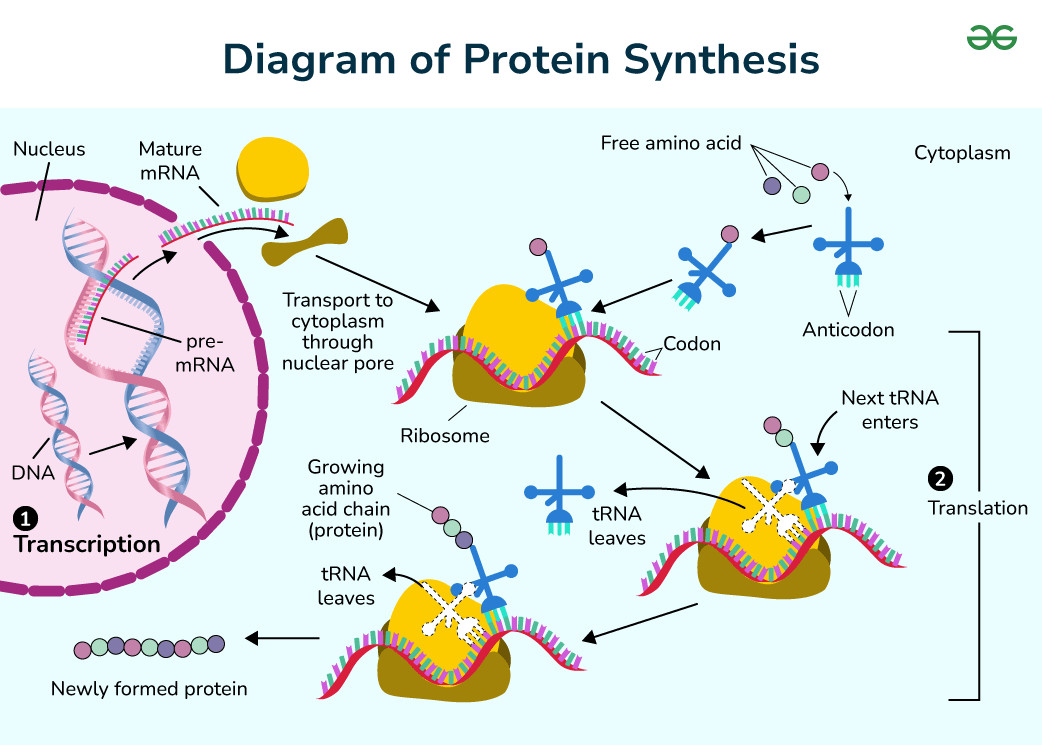
\includegraphics[width=0.9\textwidth]{resources/images/protein_synthesis.png} \\
		\caption{An illustration of the gene translation process in a cell via protein-factories known as ribosomes\cite{geeksforgeeks2024protein}}
		\label{FIG2}
\end{center}
\end{figure}
    
    
In later section (\textbf{Section \ref{SEC4}}) we shall deal with [whole] genome expression, and shall especially deal with hypothetical systems and use the modal sequence concept as the basis for exploring expression and/or manifestation of an entire organism from just its basic genetic code. In this section though, we shall focus on actual expression in real and natural biological systems, and shall focus more on expression at a molecular level --- essentially, at the level of protein manifestation via \textbf{gene expression}.

It shall be interesting to note that for genetic code in natural automata (nature-like bio-automata\footnote{My research assistant --- thanks \textbf{Microsoft Copilot}, did bring it to my attention that the term ``bio-automata" is ``usually reserved for models or conceptual representations of biological systems --- especially those designed to simulate behaviors, growth patterns, or decisions-making processes using predefined rules, like in cellular automata or agent-based modeling." And thus, much as I often find it attractive to use the term --- as an umbrella term including actual living organisms which, from the perspective of the computer scientist in me, are still correctly classifiable under the "biological automata" category in my opinion since they actually operate on some infallible inherent natural program in their DNA. But, I shall adhere to the advise of my assistant for now.} and generally living things), the most important reason the genetic coding language exists, is so that the body/host-organism system can produce required materials as and when they are needed or demanded for. This for example means producing new or extra body tissue in a still growing organism or in one with any damaged or missing tissue, and essentially, such productions are about the synthesis of particular molecules in the body's system that are basically proteins. The diagram in \textbf{Figure \ref{FIG2}} is a basic illustration of the process for living organisms --- eukaryotes especially.

For simplicity's sake, we can assume the following summarization of the basic process that fully and correctly breaks down the typical ordeal:

First, we shall assume that given the protein is just a chain of amino-acids, we might as well just think of it as though it were an ordered sequence of some terms, and thus, in keeping with the notation from transformatics, we might just refer to such a protein with our usual typical \textbf{resultant sequence} symbol --- $\Theta^*$.

And so, given that these proteins are actually nearly direct/1-to-1 mappings from the corresponding DNA sub-sequence code of a finite length, we might then refer to the DNA sequence that encodes the instructions for producing $\Theta^*$ with just the basic typical transformatics \textbf{source sequence} symbol: $\Theta$ --- more conveniently, because we wish to also talk of the length of the sequence, we might preferably write the DNA sequence code of length \textbf{n} (meaning for example, \textbf{it contains exactly n DNA-codons}), as $\Theta_n$. So, for example we might more fully express $\Theta_n$ as such:

\begin{equation}
\label{EQ1}
\Theta_n = \langle a_{ij}, \rangle ;
a_{ij} \in \psi_{DNA^*} \quad \forall j \in [1,n],  i \in [1,64] \quad \land \quad n \in \mathbb{N}
\end{equation}\\

\textbf{Equation \ref{EQ1}} being just a sometimes preferable way to write the same exact sequence as:
 
 
 \begin{equation}
\label{EQ2}
\Theta_n = \langle a_1,a_2,a_3,...,a_i,...,a_{n-1},a_n \rangle ;
\forall i \quad \exists a_i \in \psi_{DNA^*} \quad \land \quad n \in \mathbb{N}
\end{equation}\\

We have defined the special symbol sets $\psi_{DNA^*}$ in \textbf{Section \ref{SEC..}} and  $\psi_{DNA}$ in \textbf{Definition \ref{DEFDNASS}}, and as for $\psi_{DNA^*}$, we know that it essentially is the set of the distinct 64 codons (see \textbf{Table 1} in \cite{gregory1987oxford}) that \textit{especially} encode amino acids, and which were first introduced in \textbf{Section \ref{SEC1}}. Another way to expound on this is by saying that:

 \begin{equation}
\label{EQ3}
\Theta_n = \{a_i \quad | \quad a_i = \prod\limits_{\rho \in \psi_{DNA}}^3 \rho \quad \land \quad \forall i \in [1,n], n \in \mathbb{N} \quad \land \quad \psi_{DNA} = \langle A, C, G, T \rangle\}
\end{equation}\\

Thus we might encounter a gene such as $\Theta_4$ composed of exactly 4 codons as shown below:

 \begin{equation}
\label{EQ4}
\Theta_4 = \langle \langle A, T, G \rangle, \langle A, A, A \rangle, \langle T, T, A \rangle, \langle T, A, G \rangle \rangle
\end{equation}\\

Which, might also equivalently be expressed as a flattened sequence if the fact that the nucleobases it contains are always read in triplets/3-grams/tuples of 3 at a time. So that we can merely write it as:\\

 \begin{equation}
\label{EQ5}
\Theta_{4 \times 3} = \langle  A, T, G, A, A, A, T, T, A, T, A, G \rangle
\end{equation}\\

So we imply that under the flat-structure notation, the sequence has exactly $4 \times 3$ elements. By this fact and the observation that the previous nested notation merely helps to group together each codon's members within a meaningful sub-sequence, and that the order is otherwise maintained in the flat-sequence structure, we might then also equivalently express the same actual DNA code sequence as an $n \times 3$ matrix as shown below:

 \begin{equation}
\label{EQ5a}
\Theta_{4 \times 3} = \begin{pmatrix}
A& T& G\\
A& A& A\\
T& T& A\\
T& A & G \\
\end{pmatrix}
\end{equation}\\


Whether to actually express it as a $3 \times n$ matrix or as $n \times 3$ might be up to the particular taste of the mathematician or scientist, but otherwise, we know that the ordered sequence $\Theta$ in any of the forms above is essentially a \textbf{genetic program} to guide a DNA code processor such as a ribosome construct a corresponding protein based on the equivalent transcribed mRNA code sequence $\Theta_4^*$ written in mRNA code as such:


 \begin{equation}
\label{EQ6}
\Theta_4^* = \langle \langle A, U, G \rangle, \langle A, A, A \rangle, \langle U, U, A \rangle, \langle U, A, G \rangle \rangle
\end{equation}\\

Which is what we would obtain after a necessary \textbf{DNA} $\rightarrow$ \textbf{mRNA} transform attainable via a DNA sequence transformer we might define as such:\\


\begin{transf}[\textbf{DNA to mRNA Encoder}]
\label{TRANSF1}
$\Theta_n \quad \xrightarrow{O_{mRNA-encode}(\cdot)} \quad \Theta^*_n \quad;$\\
$\forall a_i \in \Theta_n = \langle a_i,\rangle:n, \quad a_i \in \psi_{DNA} \equiv \{A, T, C, G\}$,\\
and if $\exists a_i \in \Theta_n : a_i = T \implies \exists a_i^* \in \Theta^*_n: a_i^* = U$\\
Otherwise $a_i = a_i^* \implies \invpi(a_i = T \in \Theta_n) = \invpi(U \in \Theta^*_n) \quad \land \quad \invpi(\Theta_n) = \invpi(\Theta^*_n) = n$.

\end{transf}

\begin{table}[h]
  \centering
  \Large
	\begin{tabular}[t]{|c|c|c|p{3cm}|}
	\hline
	i & $a_i$ & \textbf{Amino Acid (Code-name)} & \textbf{Function}\\
	\hline
	\hline
	1 & ATG & Methionine (Met) & Start Codon: initiates translation\\
	\hline
	2 & AAA & Lysine (Lys) & Basic amino acid\\
	\hline
	3 & TTA & Leucine (Leu) & Non polar amino acid\\
	\hline
	4 & TAG & Stop (Amber) & Terminates translation\\
	
	\hline
	              
\end{tabular}
 \caption{Amino-Acid Codes and Names in $\Theta_4$, a DNA-encoded gene}
  \label{TAB1}
\end{table}

Thus, though the gene in its DNA form comprised of the ordered sequence of amino-acid codes named as in \textbf{Table \ref{TAB1}}, and yet, the resultant sequence after applying \textbf{Transformer \ref{TRANSF1}} to $\Theta_4$ would be as explained in \textbf{Table \ref{TAB2}}.


\begin{table}[h]
  \centering
  \Large
	\begin{tabular}[t]{|c|c|c|p{3cm}|}
	\hline
	i & $a_i$ & \textbf{Amino Acid (Code-name)} & \textbf{Function}\\
	\hline
	\hline
	1 & AUG & Methionine (Met) & Start Codon: initiates translation\\
	\hline
	2 & AAA & Lysine (Lys) & Basic amino acid\\
	\hline
	3 & UUA & Leucine (Leu) & Non polar amino acid\\
	\hline
	4 & UAG & Stop (Amber) & Terminates translation\\
	
	\hline
	              
\end{tabular}
 \caption{Amino-Acid Codes and Names in $\Theta_4^*$, a mRNA encoded gene}
  \label{TAB2}
\end{table}

So, note that the names (and code-names) of the mRNA encoded codons stay the same as those of their corresponding DNA-encoded codons in both tables --- this is actually generally/conventionally so. But also, note that the functions of the individual codons in either scenario are likewise expressed the same. So, this is is because, when the genetic code is actually being executed (such as in standard protein-synthesis), the processor (the ribosome) merely operates on the mRNA-encoded gene and not directly on the original DNA-encoded code sequences.

Also, important to note, the processor only produces an amino acid (as part of the protein synthesis program), only after having encountered a ``start" instruction, and we know that such instructions are the kind encoded by \textbf{start codons}, of which the most universally utilized START-codon is \textbf{ATG/AUG} known as Methionine, but also other rare-scenario\footnote{They are used less frequently, mostly in prokaryotes and some organelles. When used as START codons, they still recruit the initiator tRNA and translate as \textbf{methionine}, not their usual amino acid\cite{copilot_dna_assistant}} START-codons include the mRNA codes GUG and UUG --- used as such in prokaryotes, and then AUU and AUA, used as such in humans only. 

And then, the processor will stop the protein construction task once it encounters a gene instruction of the ``stop" kind. These are encoded using the \textbf{stop codons}, and these are strictly any one of: TAA/UAA (Ochre), TAG/UAG (Amber) and TGA/UGA (Opal)\cite{newsmedical2025startcodons}.

That said, further note that, after processing the gene, and/or after encountering a stop-codon, the ribosome (also understood as the ``protein factory") is then triggered to detach (from the ``assembly line") and then release/return the final assembled protein thus far. These resultant proteins are basically just a chain of \textbf{actual amino acids} generally starting with the Met-amino acid.

And then, further note that, in case any codons were encountered before the AUG (or rather \textit{start-codon}), these shall then be merely be skipped --- they aren't processed or won't translate into any product such as the usual case of producing an amino-acid (this, even if they would normally have triggered the production of some amino acid). 

\subsection{Protein Manufacturing Algorithm}
\label{SECPROT}

So, overall, we might sum up this critically important protein generation process with a convenient formalism such as with a protein-production algorithm expressed as in the flow-chart depicted in \textbf{Figure \ref{FIG3}}.


\begin{figure}[H]
  \begin{center}
  %\includegraphics[trim=2cm 8cm 2cm 8cm, clip, width=0.9\textwidth,]{resources/pdfs/ProteinSynthesisStateMachine.pdf}\\
   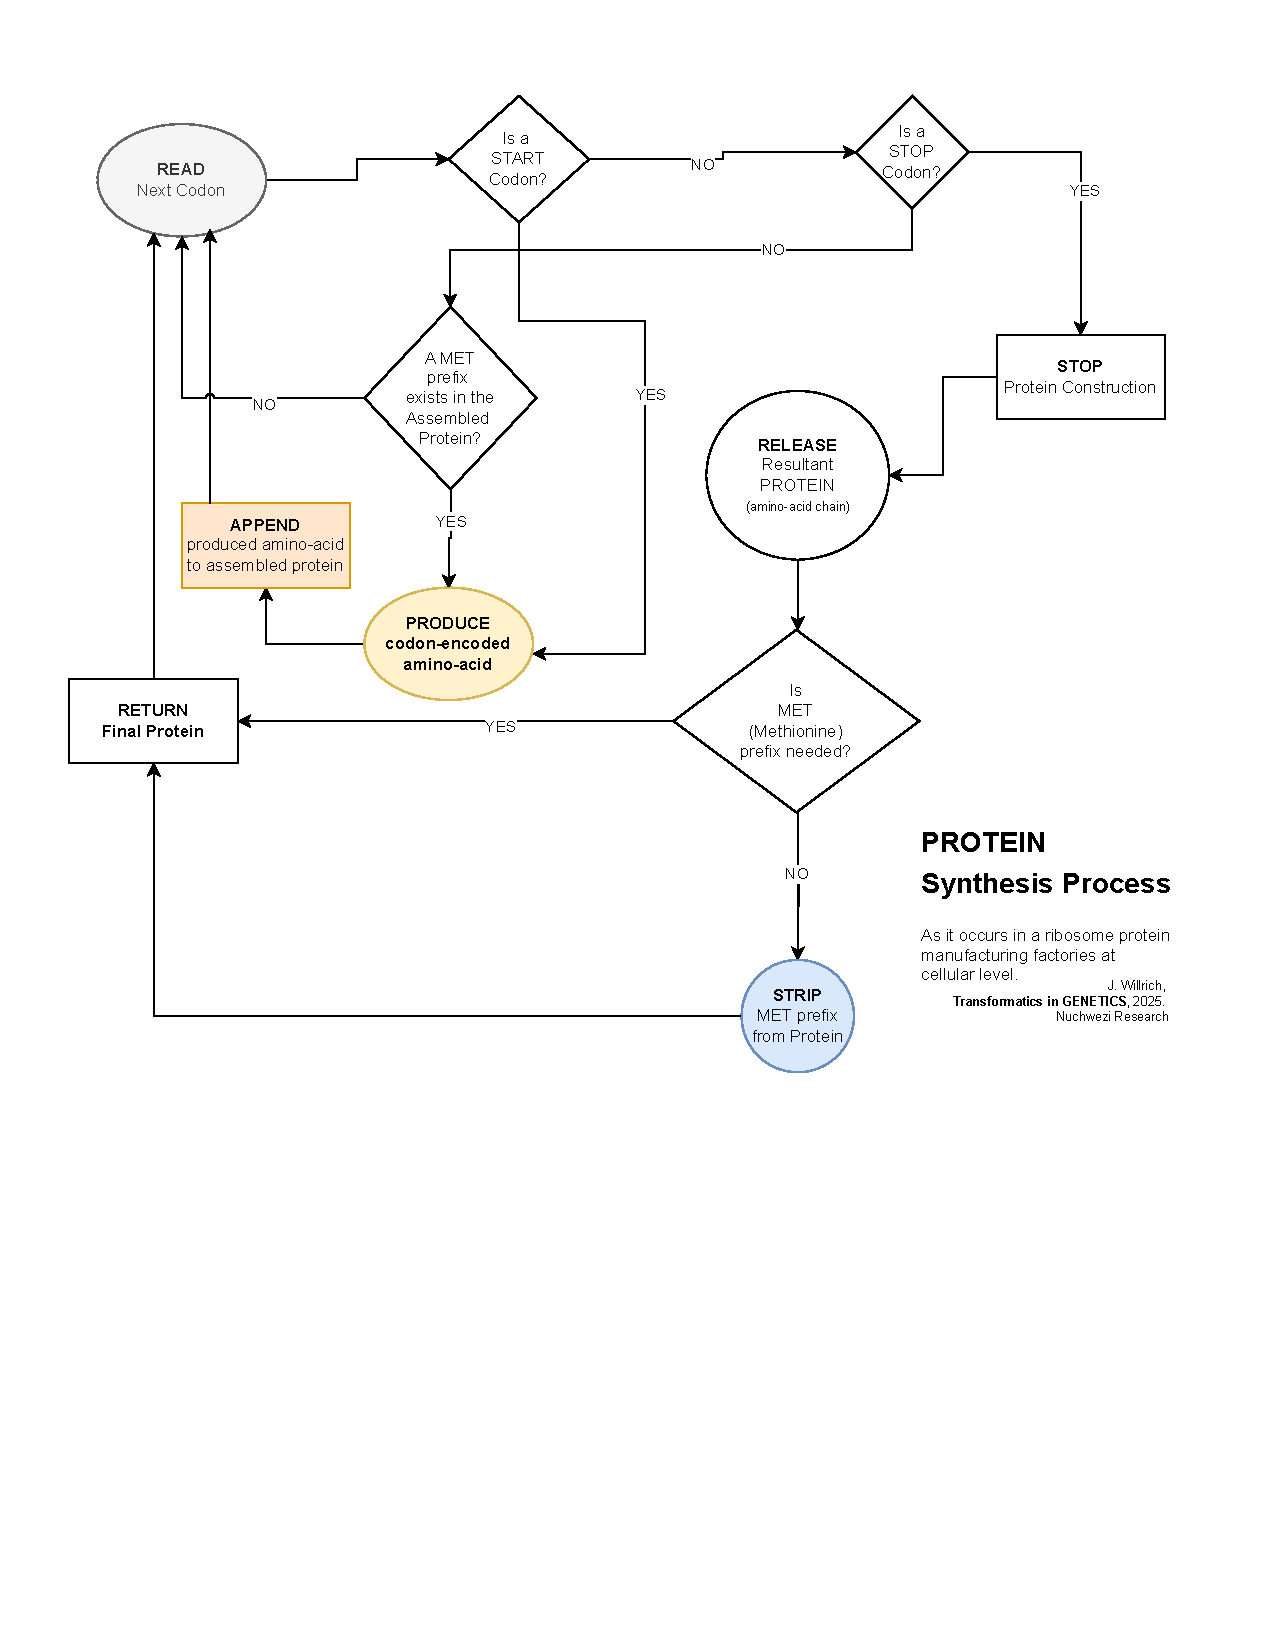
\includegraphics[trim=0cm 8cm 0cm 0cm, clip, width=0.9\textwidth,]{resources/pdfs/ProteinSynthesisProcessFlowChart.pdf}\\
   \caption{\textbf{Flow-Chart summarizing the Ribosome-based Protein-Synthesis Process in a Living Cell}}
  \label{FIG3}
  \end{center}
\end{figure}

That process which is depicted in \textbf{Figure \ref{FIG3}} is how the ribosome protein-manufacturing factory operates at a cellular level as depicted using a \textbf{Flow Chart Diagram} --- meaning, the states of the operating environment as well as those of the operator (the ribosome) are interlaced with decision-making scenarios so as to bring to mind the logic behind how the process proceeds. However, in a different diagram --- the \textbf{Ribosome State Machine} as depicted in \textbf{Figure \ref{FIG4}}, we clearly abstract everything else away and focus on what actually happens from the point-of-view of the gene code sequence processor --- the ribosome. In a way, that state machine not only depicts the various states the ribosome shall be in while operating on incoming gene-code sequences (kind of \textit{requests for solutions/solution-instances/proteins} to problems/specifications/genes) and then how it goes about producing the out-going amino-acid sequences (the proteins). It might even start to feel like the ribosome is a kind of 3D-printer, which, when presented with the specifications of a particular 3D-sequence, knows to process it (translate it) and then produce the required/specified object that is in the context of biological systems we are looking at here, essentially proteins\footnote{Of course, for someone with a background in computer science and who also has interest in designing not just computer programs but also new kinds of computers - abstract machines or not, studying the ribosome from a computing theory and computer architecture perspective --- such as so one appreciates what Instruction Set the ribosome employs; how the ribosome compares to say a Von-Neumann architecture machine; is it Turing Complete or not? How might a pure-text processing languages such as TEA\cite{lutalo2024software} implement a ribosome simulation in say a web-browser environment?\cite{lutalo_tea_web} or that failing, at least allow for the creation of a protein generator or even an entire organism generator as a simulation of how gene code sequences can be translated into sequences of multi-dimension objects?\cite{lutalo2025transformatic} etc.}.


\begin{figure}[H]
  \begin{center}
   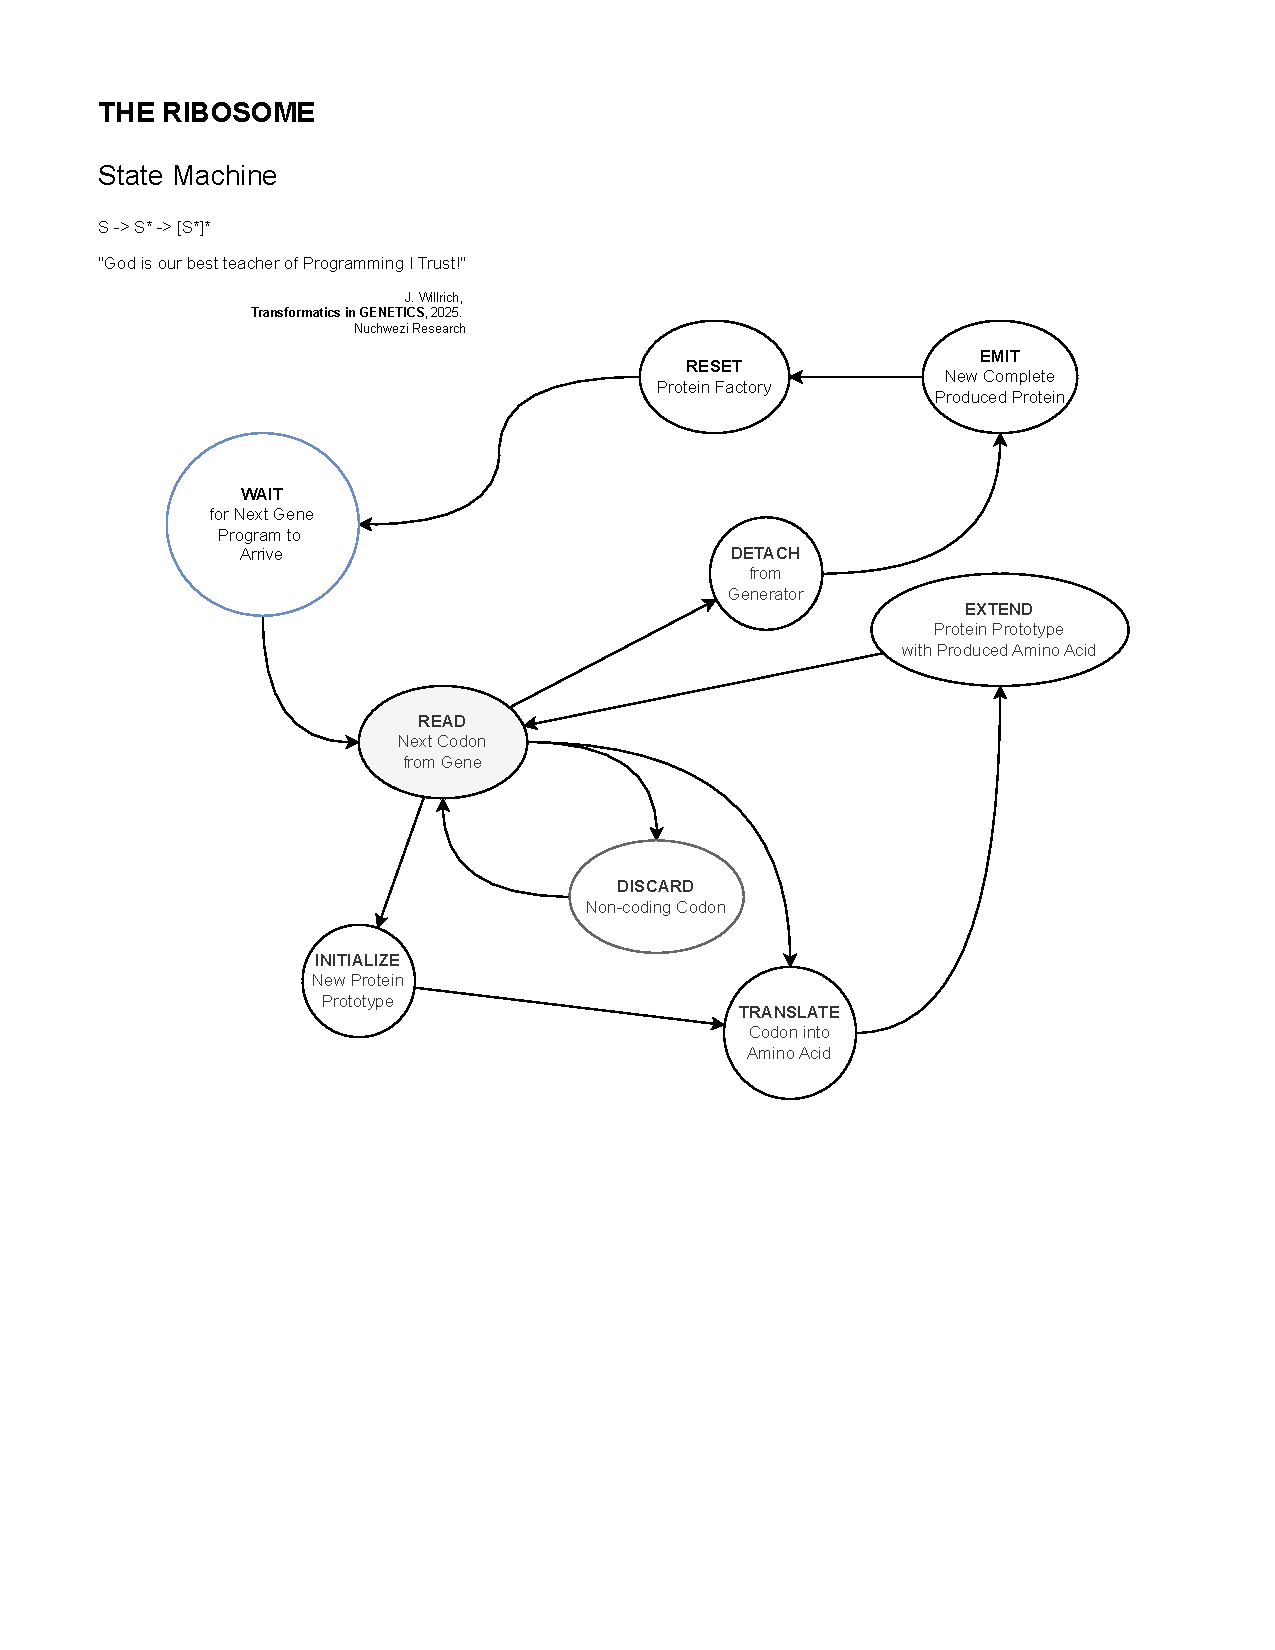
\includegraphics[trim=0cm 9cm 0cm 1.6cm, clip, width=0.9\textwidth,]{resources/pdfs/RibosomeStateMachine.pdf}\\
   \caption{\textbf{The RIBOSOME State Machine}}
  \label{FIG4}
  \end{center}
\end{figure}


Before concluding this section on biological computing systems of the sequence generator kind\cite{lutalo2025transformatic}, it should be worthwhile noting that, as depicted in \textbf{Figure \ref{FIG4}}, the process that is naturally found in every living thing's tiniest cells (excluding viruses as already saw in \textbf{Section \ref{SEC1}}, could be, as with any legitimate state machine, be used to implement a proof-of-concept ribosome processor (or a \textit{ribosome computer} --- a way to implement bio-automatons that behave like a ribosome or which process code similar to DNA and mRNA, or which generally operate on sequences to produce other (possibly more complex) sequences. Thinking of a robotic ribosome might not be something that is immediately required in contemporary medicine or in-organism computing systems, but might be a concept worth adapting or exploring for the design and implementation of self-contained robotic factories for manufacturing and outputting complex products producible via use of a sequence-processing, assembly-line kind of method just as proteins are produced in a bio-cell by the ribosome. We might for example think of ``a sequence from which a finished particular type of car can be manufactured at will" or ``a sequence from which certain kinds of sequence-form/sequence-based\footnote{Vertebrates anyone(?)} artificial and/or organic creatures or bots might be systematically produced at will or on-demand". These kinds of printers --- which, unlike just printers of things on paper, or 3D-printers that know to only produce plastic variants of models they are fed with, but which can say \textit{print a human}\footnote{Though we might touch on it in a future paper on philosophy --- e.g in \textit{Computational Mysticism}\cite{lutalo2024mysticism}, it might be interesting to air-out the author's illuminating view that unlike most other bio-mata such as beasts in the wild or fish in the seas, and definitely not as with silicon-based automatons such as GPT-powered modern \textit{disincarnate} artificial entities --- nor the likes of the ZHA qAGI\cite{jwlzha}, that the human in particular, has this peculiar attribute to them that, apart from just their material substratum as any physical robot might possess or need --- and which is say the domain of ``material producers" such as the ribosome is, and away from their conceptual/software substratum too, they seem to, or perhaps arguably, also possess a preternatural layer of existence that perhaps is or might not have anything to do with their DNA/material-blueprint. A better or more precise classification term for such [\textit{preter-}]intelligent -mata/matter(?) might be the still underground term and concept of a \textit{Psymaton} or \textbf{Psymata} --- bits of this line of discourse have been already touched on in the Psymaz Interview\cite{lutalo2025unraveling}.}, teleport a cow or a banana, etc. might be interesting to explore, as we look into the far-future, where, with humanity's ability to travel and survive in remote and/or unnatural worlds away from their biological home environments (such as Earth's biosphere), might compel them to have to develop new kinds of machines that would not only print out ideas on paper, but also complete food ready-to-eat, medicines to particular kinds of ailments, certain kinds of companion creatures or species, etc. Means to survive on/in alien worlds by leveraging smart, general sequence processors and generators. Talking of which, the next section shall help us start to appreciate this perspective of using the case of genetic code sequences and the ribosome sequence processor into the dimension of both artificial as well as conceptual or hypothetical bio-machines that like the bio-cell can produce complex things via processing of some kinds of code sequences. Bio-automata.

\subsection{Gene Expression in Living Things and for Bio-Automata via Ribosomes}
\label{SEC5}

One might begin by wondering: \textbf{using the concepts from transformatics and pure mathematics, how might we model or express a general and realistic ribosome?} 

A plausible and meaningful solution to this problem would be to begin by acquiring or developing \textit{a rigorous and correct working definition of what a ribosome is.} The answer would follow directly from that, thus our first definition in this section; a formal definition of a ribosome in any system natural or artificial:


%\fbox{\begin{minipage}{0.9\textwidth}

\begin{defn}[A \textbf{Ribosome}]
\label{DEFRIBOSOME}
Assuming we re-write a sequence of DNA code in terms of the ordered sequence of nucleotides it contains, as in \textbf{Equation \ref{EQ3}} re-written as in \textbf{Equation \ref{EQ7}}:

 \begin{equation}
\label{EQ7}
\Theta_n = \{a_i \quad | \quad a_i = \prod\limits_{\rho \in \psi_{DNA}}^3 \rho \}:n
\end{equation}\\

$\Theta_n$ would then be any sequence of DNA-codons of length $n$, equivalent to an equivalent flat-structure ordered sequence of nucleotides of length $n \times 3$. We can then produce mRNA-codons from $\Theta_n$ as per \textbf{Transformer \ref{TRANSF1}}, so that we produce a new mRNA-codon sequence of length $n$ that is generated as such:

\begin{trans}
\label{TRANS1}
$\Theta_n \quad \xrightarrow{O_{mRNA-encode}(\cdot)} \quad \Theta^*_n;$\\
$\Theta^*_n = \{a_i^* \quad | \quad a_i^* = \prod\limits_{\rho \in \psi_{mRNA}}^3 \rho \}:n$
\end{trans}

And with $\Theta^*_n$ produced, we can then merely generate the corresponding ordered sequence of amino-acids, denoted as $[\Theta^*_n]^*$, via the following mRNA to amino-acid transformer: 

\begin{transf}[\textbf{mRNA to Amino-Acid Translator}]
\label{TRANSF2}
$\Theta^*_n \quad \xrightarrow{O_{mRNA-translate}(\cdot)} \quad [\Theta^*_n]^* \quad;$\\
\begin{enumerate}
\item $\invpi([\Theta^*_n]^*) < \invpi(\Theta^*_n)$ because we only count each codon in the source once, and as per the rules of gene processing/transcription, all non-coding codons (introns) --- basically, codons not able to be translated into an amino-acid given the state of the gene processor\footnote{See \textbf{Figure \ref{FIG3}} and \textbf{Figure \ref{FIG4}}}, don't contribute to the generated resultant sequence in terms of sections it contains --- with the exception of the special ``Met" codon\footnote{A START-codon also counted among genuine ``exons" --- coding codons} that might or might not be retained in the resultant sequence even though it is automatically included as the first produced amino-acid in any legitimate gene sequence.
\item The entire sequence $[\Theta^*_n]^*$ is a kind of 3-Dimension molecule based on the chain of amino-acids it contains, and is technically referred to as a protein.
\end{enumerate}
$\qed$
\end{transf}

A \textbf{Ribosome} then, is any combination of transformers that can result in $[\Theta^*_n]^*$ when presented with just $\Theta_n$ as per the two intermediate transformer processes \textbf{Transformer \ref{TRANSF1}} and \textbf{Transformer \ref{TRANSF2}}, and whose overall processing algorithm is as depicted in \textbf{Figure \ref{FIG3}} and its corresponding state machine as in \textbf{Figure \ref{FIG4}}. 

So, overall, a ribosome is any machine that can implement the combined transformer defined as in \textbf{Transformer \ref{TRANSF3}}:

\begin{transf}[The \textbf{Protein Generator} (A Ribosome)]
\label{TRANSF3}
$\Theta_n  \xrightarrow{O_{mRNA-encode}(\cdot)}  \Theta^*_n  \xrightarrow{O_{mRNA-translate}(\cdot)} [\Theta^*_n]^*;$\\
$\invpi([\Theta^*_n]^*) < \invpi(\Theta^*_n) = \invpi(\Theta_n) = n:$\\
$\psi_{\Theta} = \psi_{DNA} \quad \land \psi_{\Theta^*_n} = \psi_{mRNA} \quad \land \psi([\Theta^*_n]^*) = \psi_{amino-acids}$
\end{transf}

And thus, we can finally merely call any machine capable of implementing the protein generator  in \textbf{Transformer \ref{TRANSF3}} as a \textbf{Ribosome}.

\end{defn}

%\end{minipage}}
%\\

\section{Transformatics and Genome Expression in Bio-Automata}
\label{SEC4}

\begin{quotation}
\noindent \texttt{Genome Expression: The collective expression profile of all genes within a genome, including coding and non-coding regions, across different conditions, cell types, or developmental stages. It is a systems-level view --- measuring how the entire genome behaves dynamically. This includes: mRNA expression of all genes, non-coding RNA activity, epigenetic regulation, chromatin accessibility and transcriptional networks. In essence, gene expression is local, while genome expression is global.}\\
\hspace*{\fill} --- \textbf{Microsoft Copilot}\cite{copilot_dna_assistant}
\end{quotation}

Away from using transformatics to make sense of the differences between organisms based on their genetic code sequences, an even more exciting application of the theory and practical methods of transformatics would be in conceptualizing, analyzing and explaining the important biological, physical, chemical, informational and mathematical concept of \textbf{genome expression}. We shall use a thought experiment and hypothetical cases leveraging exemplary genetic code modeled using special sequences that are treated as modal sequences at minimum.

First, we shall define a basic cipher that can encode the basic digits (of base-10), as some unique, but non-digit forms (essentially, with non-digit \textit{glyphs}). This, so when we speak of a living organism --- for example a pine-apple or a feline, we don't expect that in nature, or rather, that by physically dissecting the organism, that one shall find trapped or stored inside it, the literal genetic code symbols (such as those in $\psi_{na}$), but rather, that they shall find natural literal expressions or instances of genetic code material basis --- such as the chemical base molecules that define nucleobases, or nucleotides, and also complex molecular structures such as transcribed amino-acids post-RNA translation of DNA expressions.

So, in our hypothetical genome expression model, we are going to expect elements from our basic hypothetical DNA symbol set:

\begin{equation}
\label{EQHYPDNASS}
\psi_{\Omega} = \langle 0, 1, 2, 3, 4, 5, 6, 7, 8, 9 \rangle \equiv \psi_{10}
\end{equation}

Which, especially for curiosity's sake, but also, for creative and expressive reasons, is meant to allow us to explore a peculiar genetics model based on not just some four base symbols as is the case in $\psi_{DNA}$, but which allows us to look at any base-10 number expression as a potential genetic code sequence with \textbf{each digit expressing a distinct hypothetical nucleic acid}. For example, we might describe some fictitious organism --- for simplicity's sake, perhaps just a virus that we shall name \textbf{the Euler Virus}\footnote{We called it that, simply because of the fact the associated genome sequence is based on the important natural physical constant --- 2.718281828459, the \textbf{Euler number}, that is one of those irrational numbers that also happens to be the base of the natural logarithm and which arises naturally in many areas of mathematics, especially in calculus, complex analysis, and probability theory.} or just ``veuler", as having its entire genome sequence encoded as just:

\begin{equation}
\label{EQDNAV}
\Omega_{veuler} = 27182818
\end{equation}


However, that is the DNA-side of the story. As in real nature, we need a \textit{different} alphabet or symbol set for expressing genetic code in its \textit{intermediate form} --- as genome expression typically proceeds via expression of DNA into mRNA first of all, and then finally into functions such as proteins. So, in our case, the intermediate expressions shall be expressed using the \textbf{Ozin Cipher}\footnote{More about this in the \textbf{\hyperref[APPOZIN]{Appendix}}.}, which we are to describe hereafter.


\subsection{The Ozin Genetic Code Cipher}
\label{SECOZIN}

With the background we have obtained thus far, note that the special \textbf{transcription level} expression of our genetic code originally expressed via $\psi_{10}$, shall be transcribed into the intermediate \textbf{ozin genetic code} that spans the symbol set $\psi_{oz}$ that is mapped from the genetic code storage expression via a mapping as depicted in \textbf{Figure \ref{FIGOZIN}}.




\begin{figure}[H]
  \begin{center}
  %\includegraphics[trim=2cm 8cm 2cm 8cm, clip, width=0.9\textwidth,]{resources/pdfs/ProteinSynthesisStateMachine.pdf}\\
   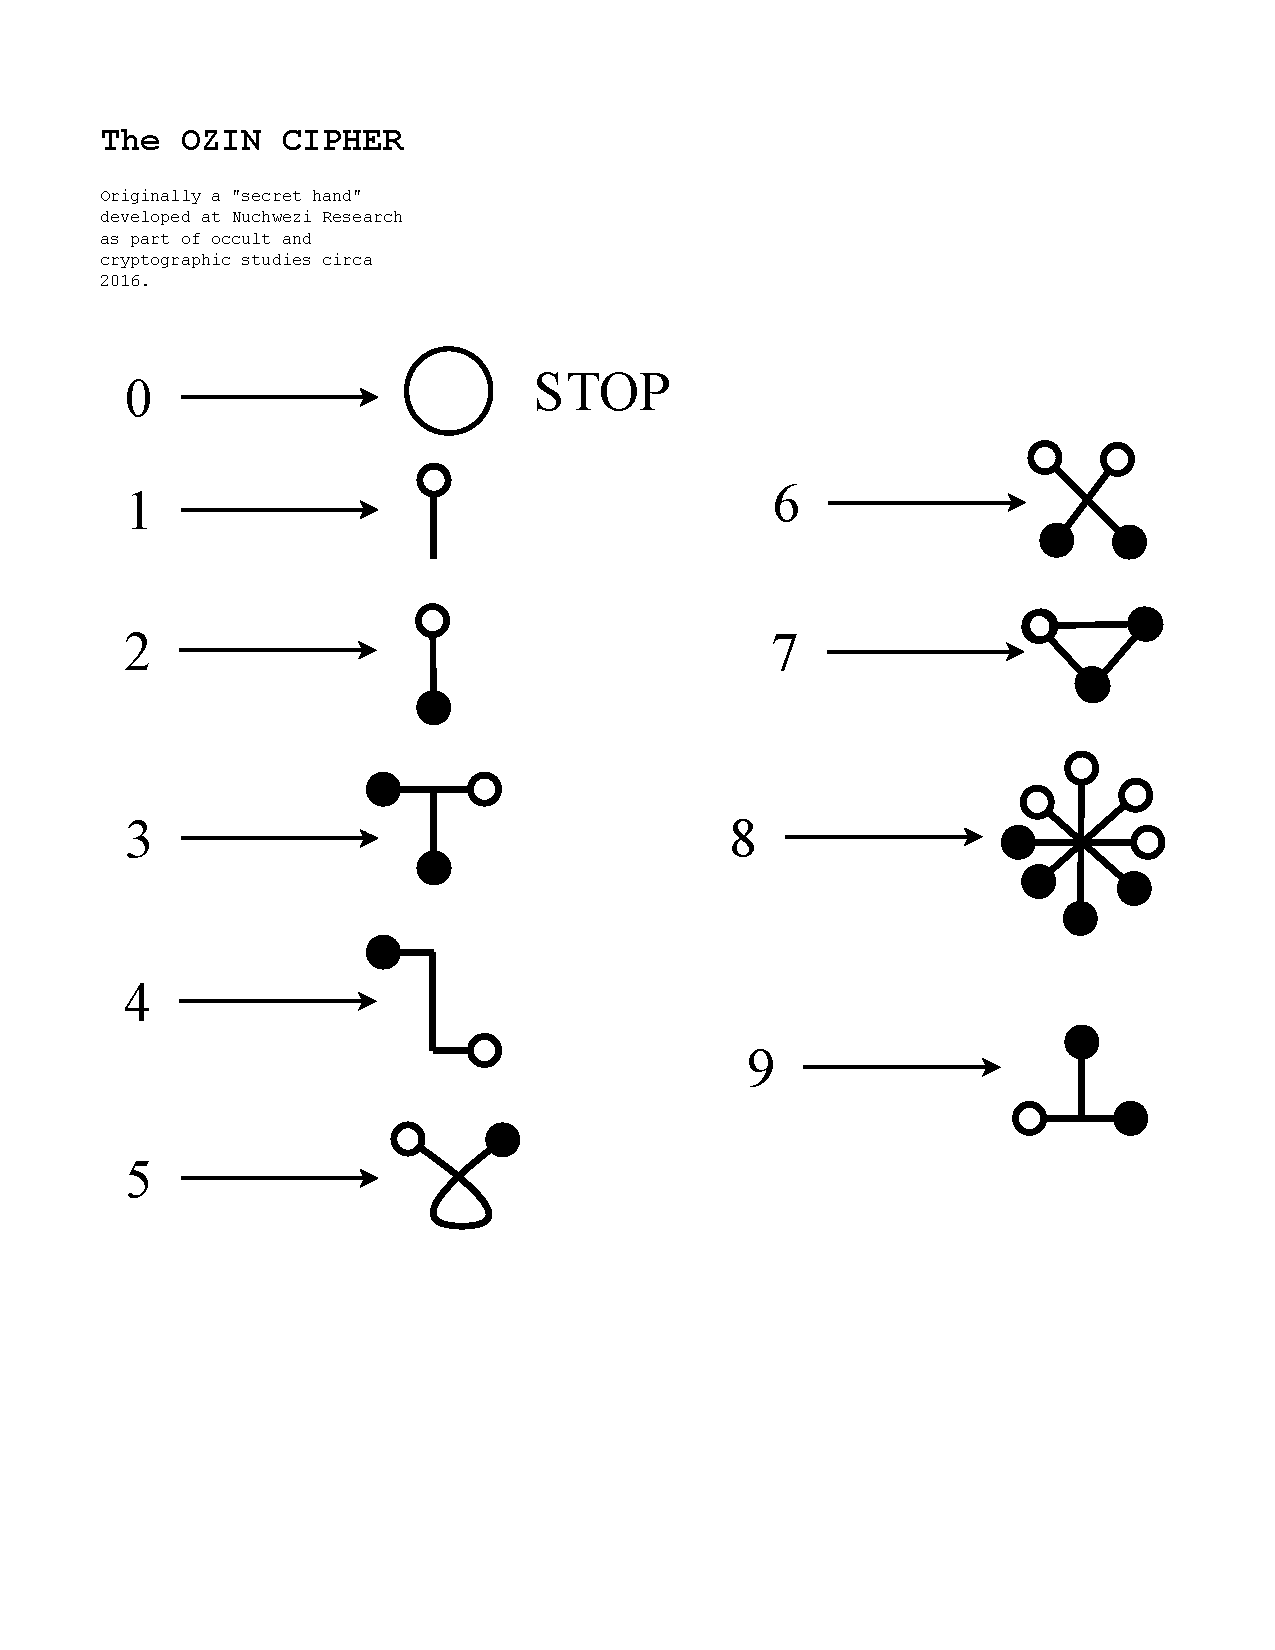
\includegraphics[trim=0cm 6cm 0cm 0cm, clip, width=0.9\textwidth,]{resources/pdfs/OZINCIPHER.pdf}\\
   \caption{The OZIN Cipher mapped from Decimal Symbols.}
  \label{FIGOZIN}
  \end{center}
\end{figure}


For simplicity's sake, we might interpret or transcribe from base-$\Omega$ DNA into our base-OZ RNA expression as such:

If for some organism such as that expressed via $\Omega_{veuler} = 27182818$, we wish to encode the equivalent intermediate [physical] expression, then we iterate through each symbol in the source code sequence, and re-write it as the equivalent symbolic structure in OZIN, and this, so as to center the ozin glyphs along a \textbf{backbone structure} of just a mere line that starts with a tiny dot and ends with the last ozin structure from the source sequence transcribed. Essentially, for our Euler Virus, it would render as something of the sort shown in \textbf{Figure \ref{FIGOZEVIRUS}}

\begin{figure}[H]
  \begin{center}
  %\includegraphics[trim=2cm 8cm 2cm 8cm, clip, width=0.9\textwidth,]{resources/pdfs/ProteinSynthesisStateMachine.pdf}\\
   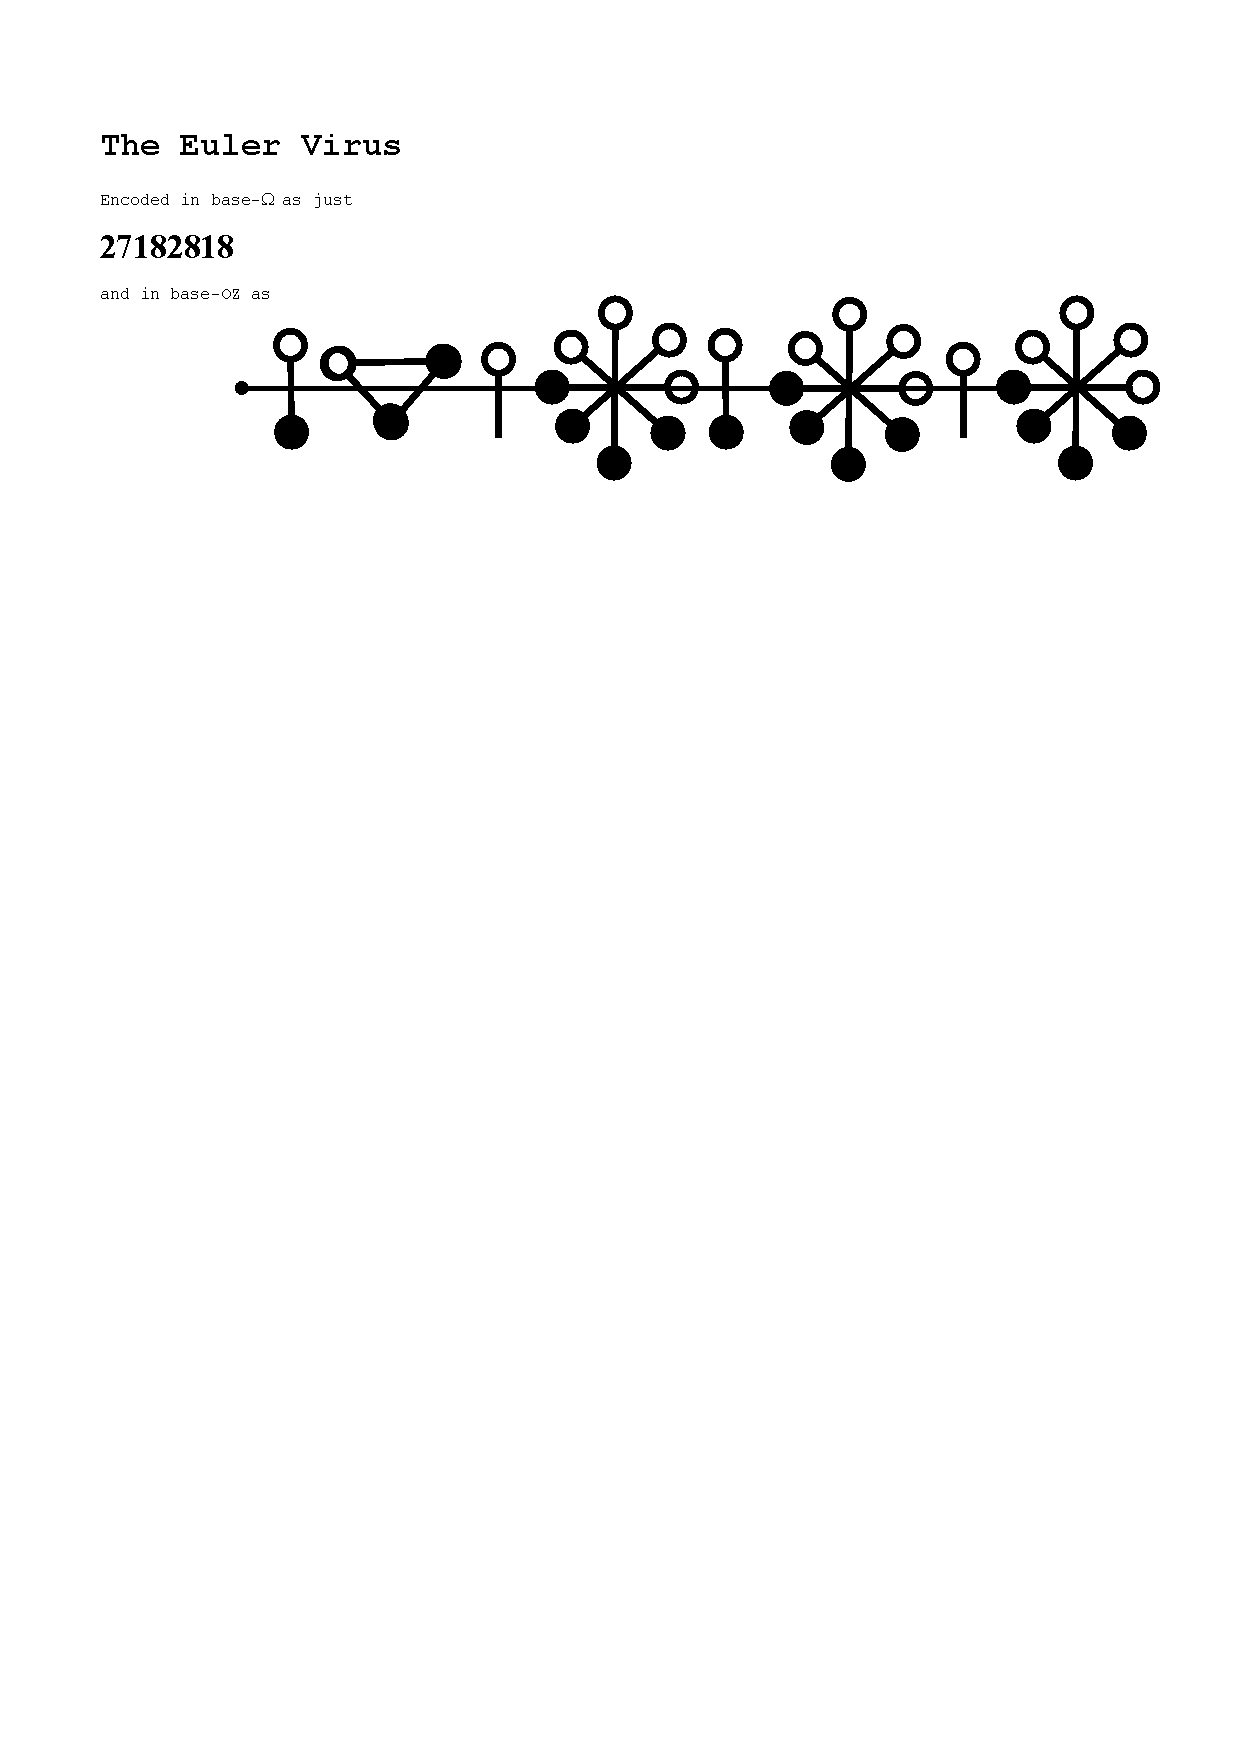
\includegraphics[trim=0cm 20cm 0cm 0cm, clip, width=0.9\textwidth,]{resources/pdfs/OZINCIPHER-APP1-EVIRUS.pdf}\\
   \caption{The equivalent OZIN expression of the hypothetical Euler Virus genome sequence.}
  \label{FIGOZEVIRUS}
  \end{center}
\end{figure}


Another organism, which we might just refer to as the \textbf{HiFinelle}, is actually based off of our favorite base-10 o-SSI --- the \textbf{Hi-Fi o-SSI}\cite{adtpaper}, and thus, its corresponding genetic code at rest is as:


\begin{equation}
\label{EQDNHIFI}
\Omega_{HiFinelle} = 8649137520
\end{equation}


And which, after we have it transcribed into intermediate OZIN genetic expression, shall appear as shown in \textbf{Figure \ref{FIGOZHIFI}}


\begin{figure}[H]
  \begin{center}
  %\includegraphics[trim=2cm 8cm 2cm 8cm, clip, width=0.9\textwidth,]{resources/pdfs/ProteinSynthesisStateMachine.pdf}\\
   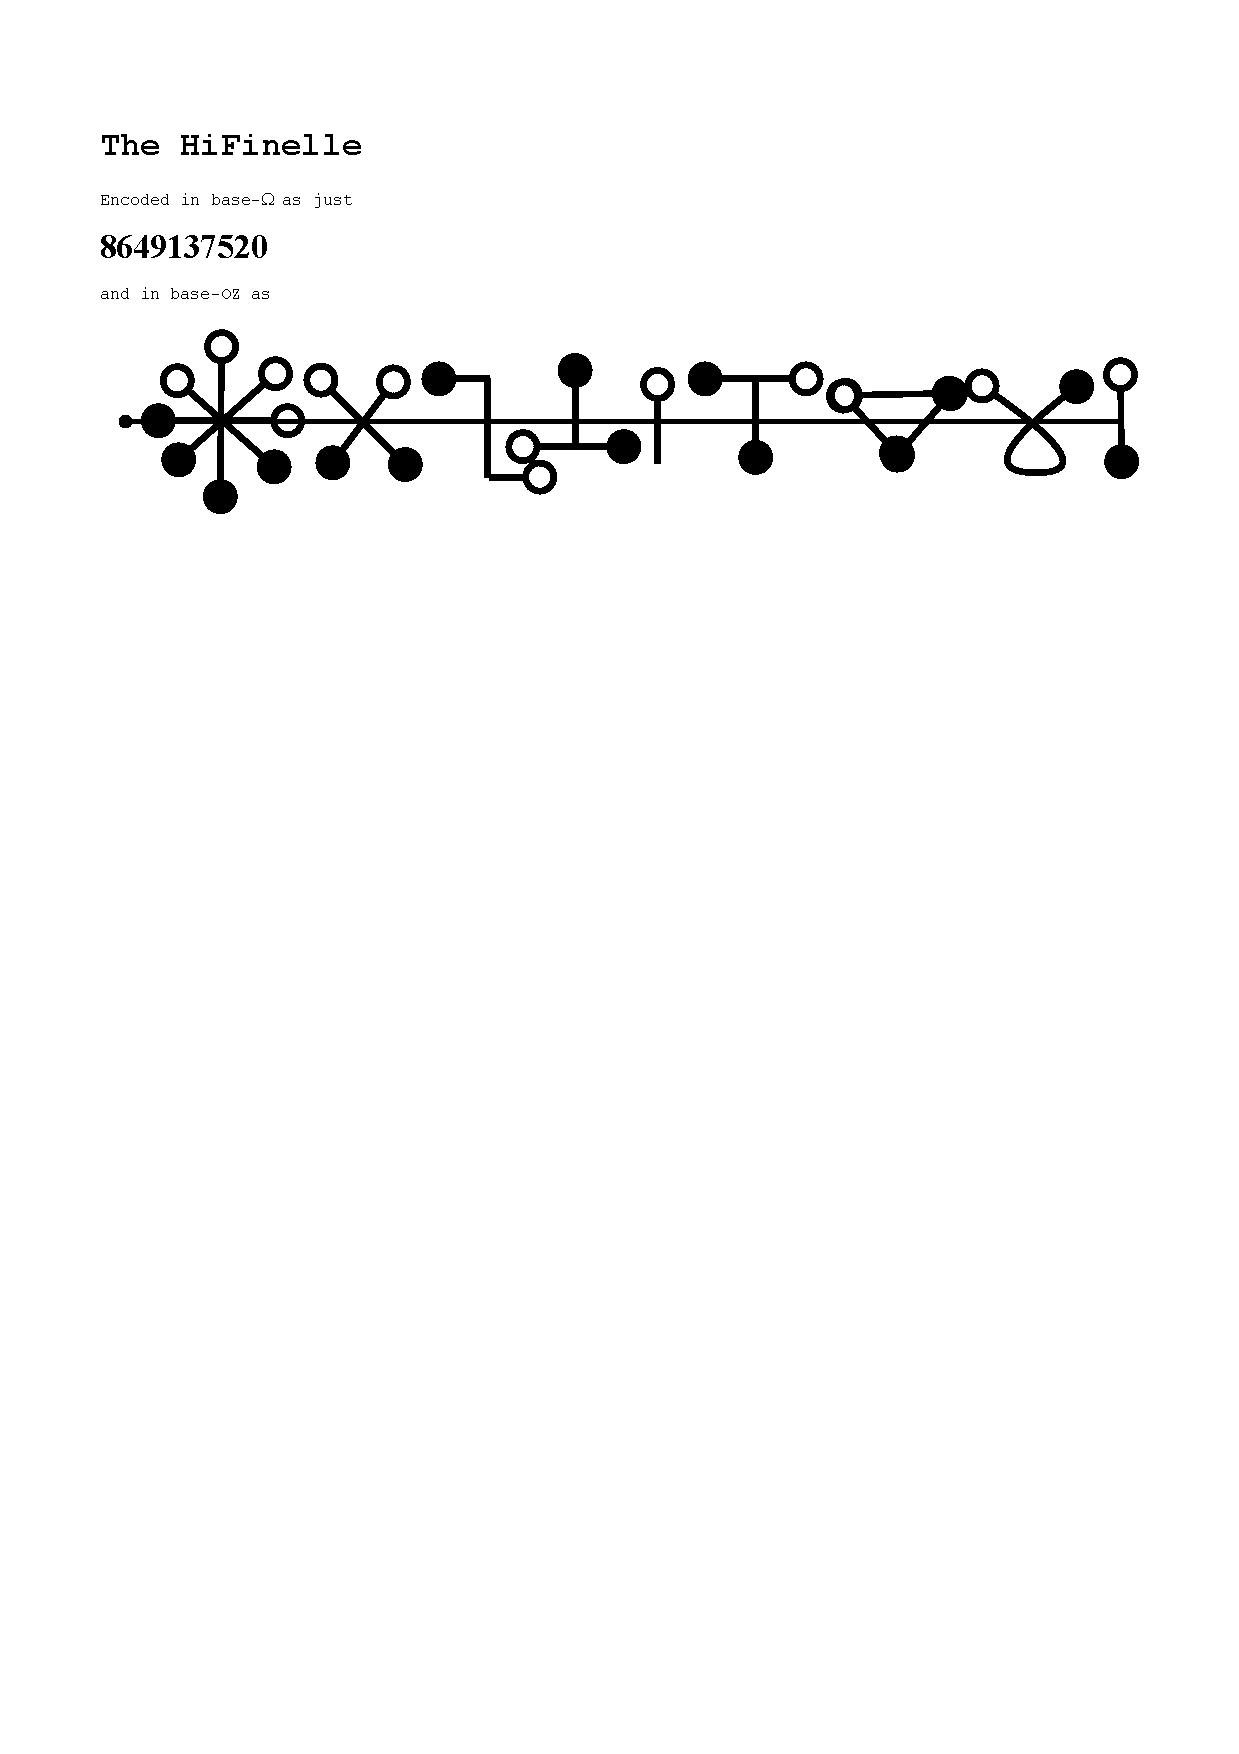
\includegraphics[trim=0cm 20cm 0cm 0cm, clip, width=0.9\textwidth,]{resources/pdfs/OZINCIPHER-APP2-HIFINELLE.pdf}\\
   \caption{The equivalent OZIN expression of the HiFinelle genome sequence.}
  \label{FIGOZHIFI}
  \end{center}
\end{figure}

Of course, in our simplistic genome expression system, the occurrence of that last ``0" symbol in the HiFinelle genome sequence tells us to STOP or just exclude that symbol with a GAP in case any other symbols follow thereafter. It is our STOP-codon equivalent.

Another genome sequence, 

\begin{equation}
\label{EQDNEXA}
\Omega_{3} = 0123026
\end{equation}

Might help illustrate that point --- see \textbf{Figure \ref{FIGOZEXA}}


\begin{figure}[H]
  \begin{center}
  %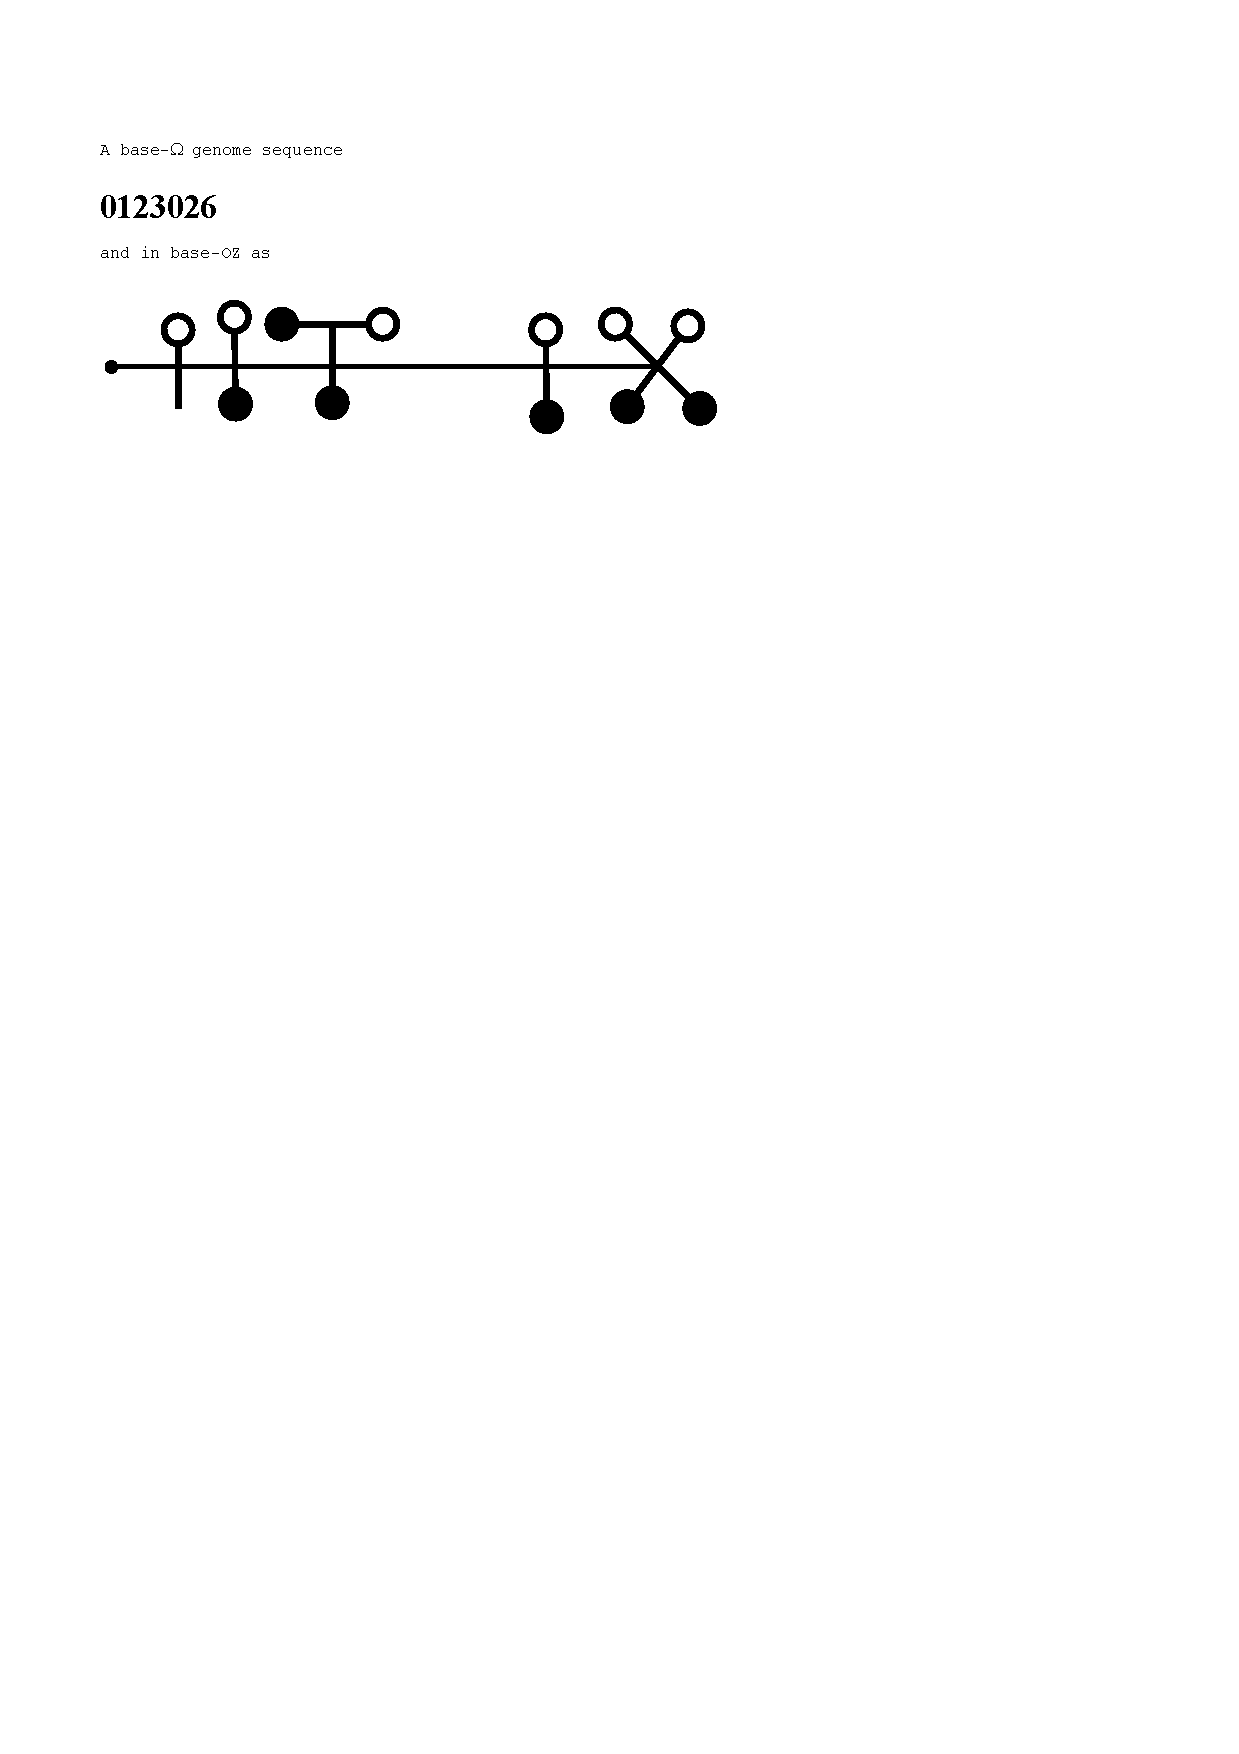
\includegraphics[trim=0cm 20cm 0cm 0cm, clip, width=0.9\textwidth,]{resources/pdfs/OZINCIPHER-APP3-EXA.pdf}\\
   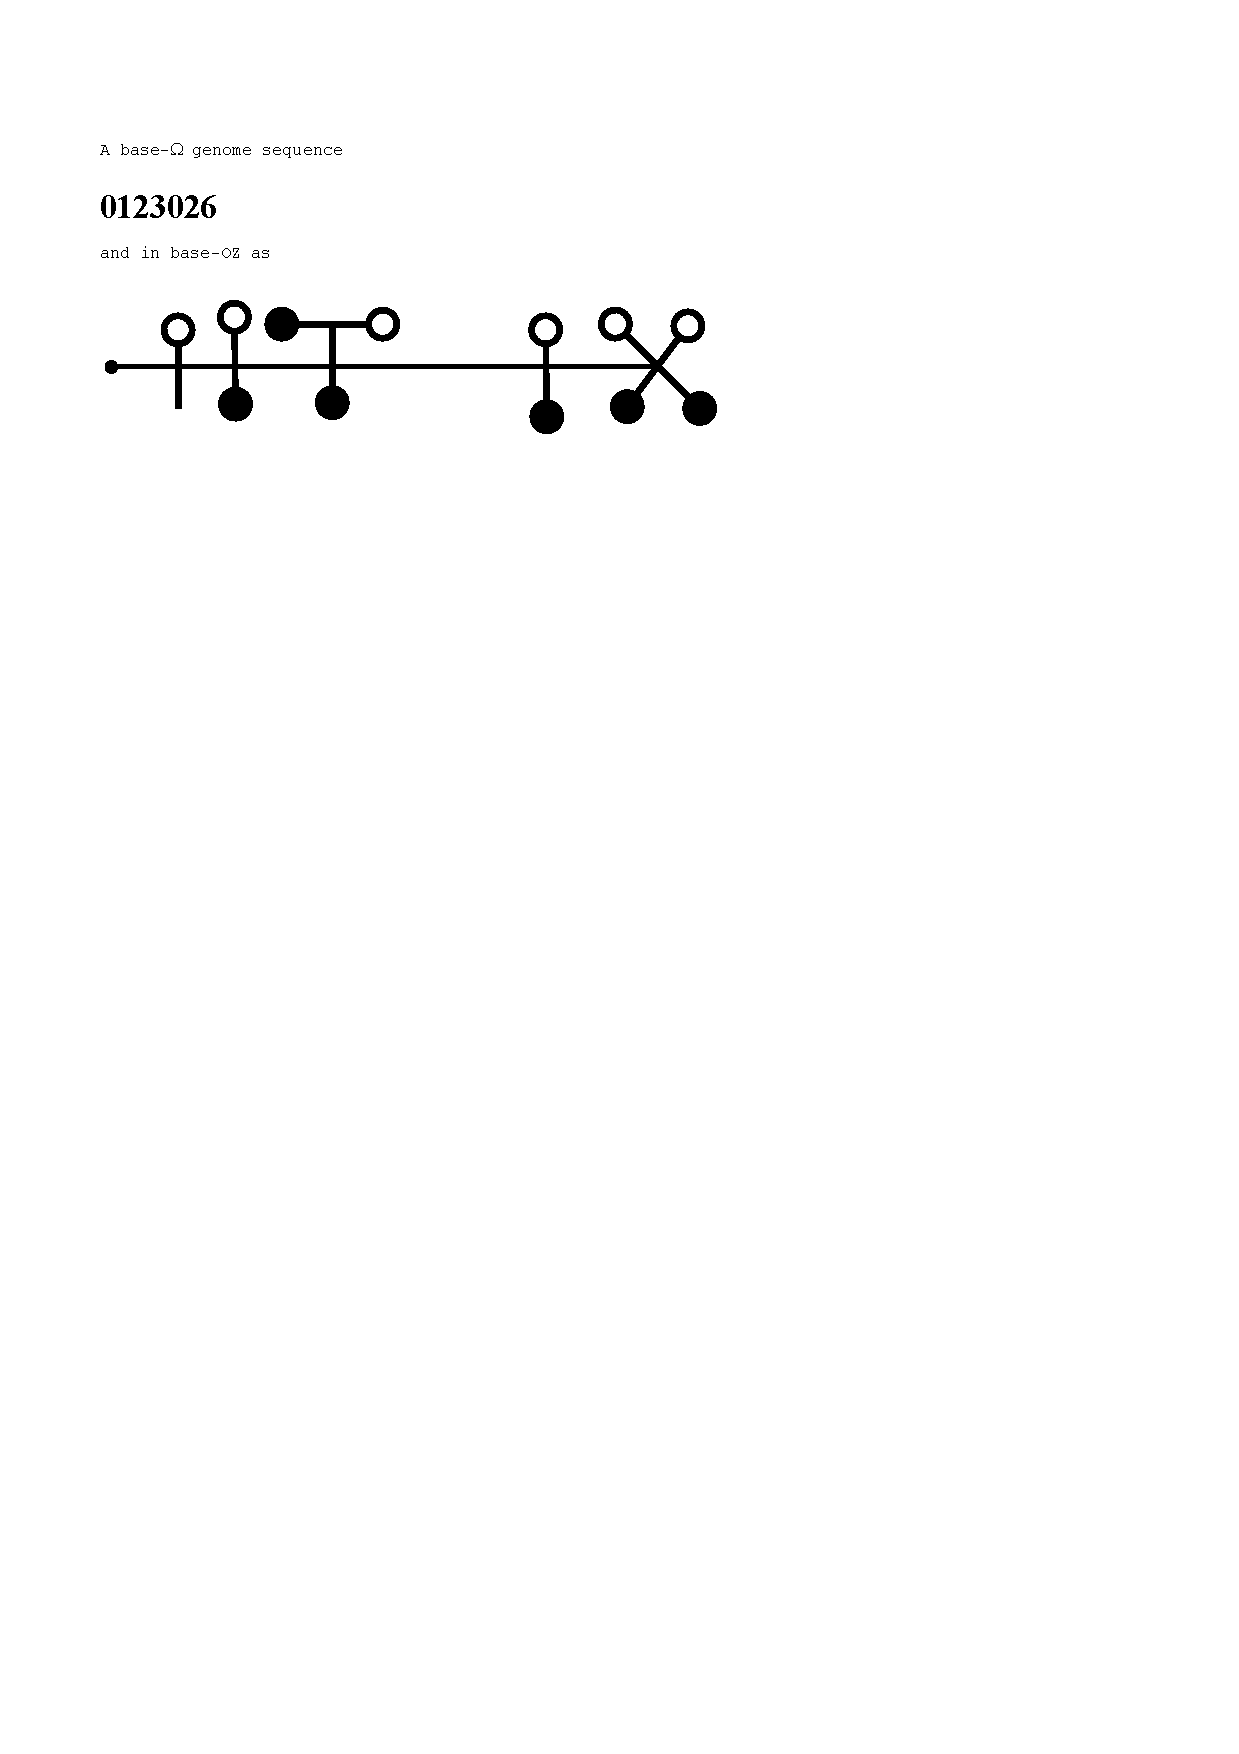
\includegraphics[trim=0cm 22cm 7cm 5cm, clip, width=0.9\textwidth,]{resources/pdfs/OZINCIPHER-APP3-EXA.pdf}\\
   \caption{The equivalent OZIN expression of the $\Omega_{3}$ genome sequence.}
  \label{FIGOZEXA}
  \end{center}
\end{figure}

That aside, in \textbf{Section \ref{SEC3A}}, we have looked at not just the interesting idea of [genetic code] sequence complements, but have also explored several applications of the idea in \textbf{Section \ref{SECAPPCOMPLEMENTS}}, including the concept of the equivalence of sequences under the complement transform. Talking of which, assuming we had a special genome sequence that is made up of subsequences that are complements of each other (such as we might call \textbf{palindromic na-Sequences}) --- e.g $\Theta_{pal}$ defined below, that is actually a palindrome of the two DNA codons --- \textbf{ATG} (Methionine) and \textbf{CAA} (Glutamine) --- the complements being \textbf{GTA} (Valine) and \textbf{AAC} (Asparagine)\cite{wikipedia_codon_tables}.

\begin{equation}
\label{GENOMEPAL}
\Theta_{pal} = \langle A, T, G, C, A, A, A, A, C, G, T, A \rangle
\end{equation}

If we express $\Theta_{pal}$ in our special numeric \textbf{base-$\Omega$}, and then into the visual \textbf{base-OZ}, we shall get something like $\Omega_{pal}$\footnote{Simplified, so we can easily visualize it in base-OZ}:

\begin{equation}
\label{GENOMEPALOMEG}
\Omega_{pal} = \langle 1, 2, 3, 3, 2, 1 \rangle
\end{equation}

And which, if we transcribe it into the intermediate OZIN code, we get:



\begin{figure}[H]
  \begin{center}
  %\includegraphics[trim=2cm 8cm 2cm 8cm, clip, width=0.9\textwidth,]{resources/pdfs/ProteinSynthesisStateMachine.pdf}\\
   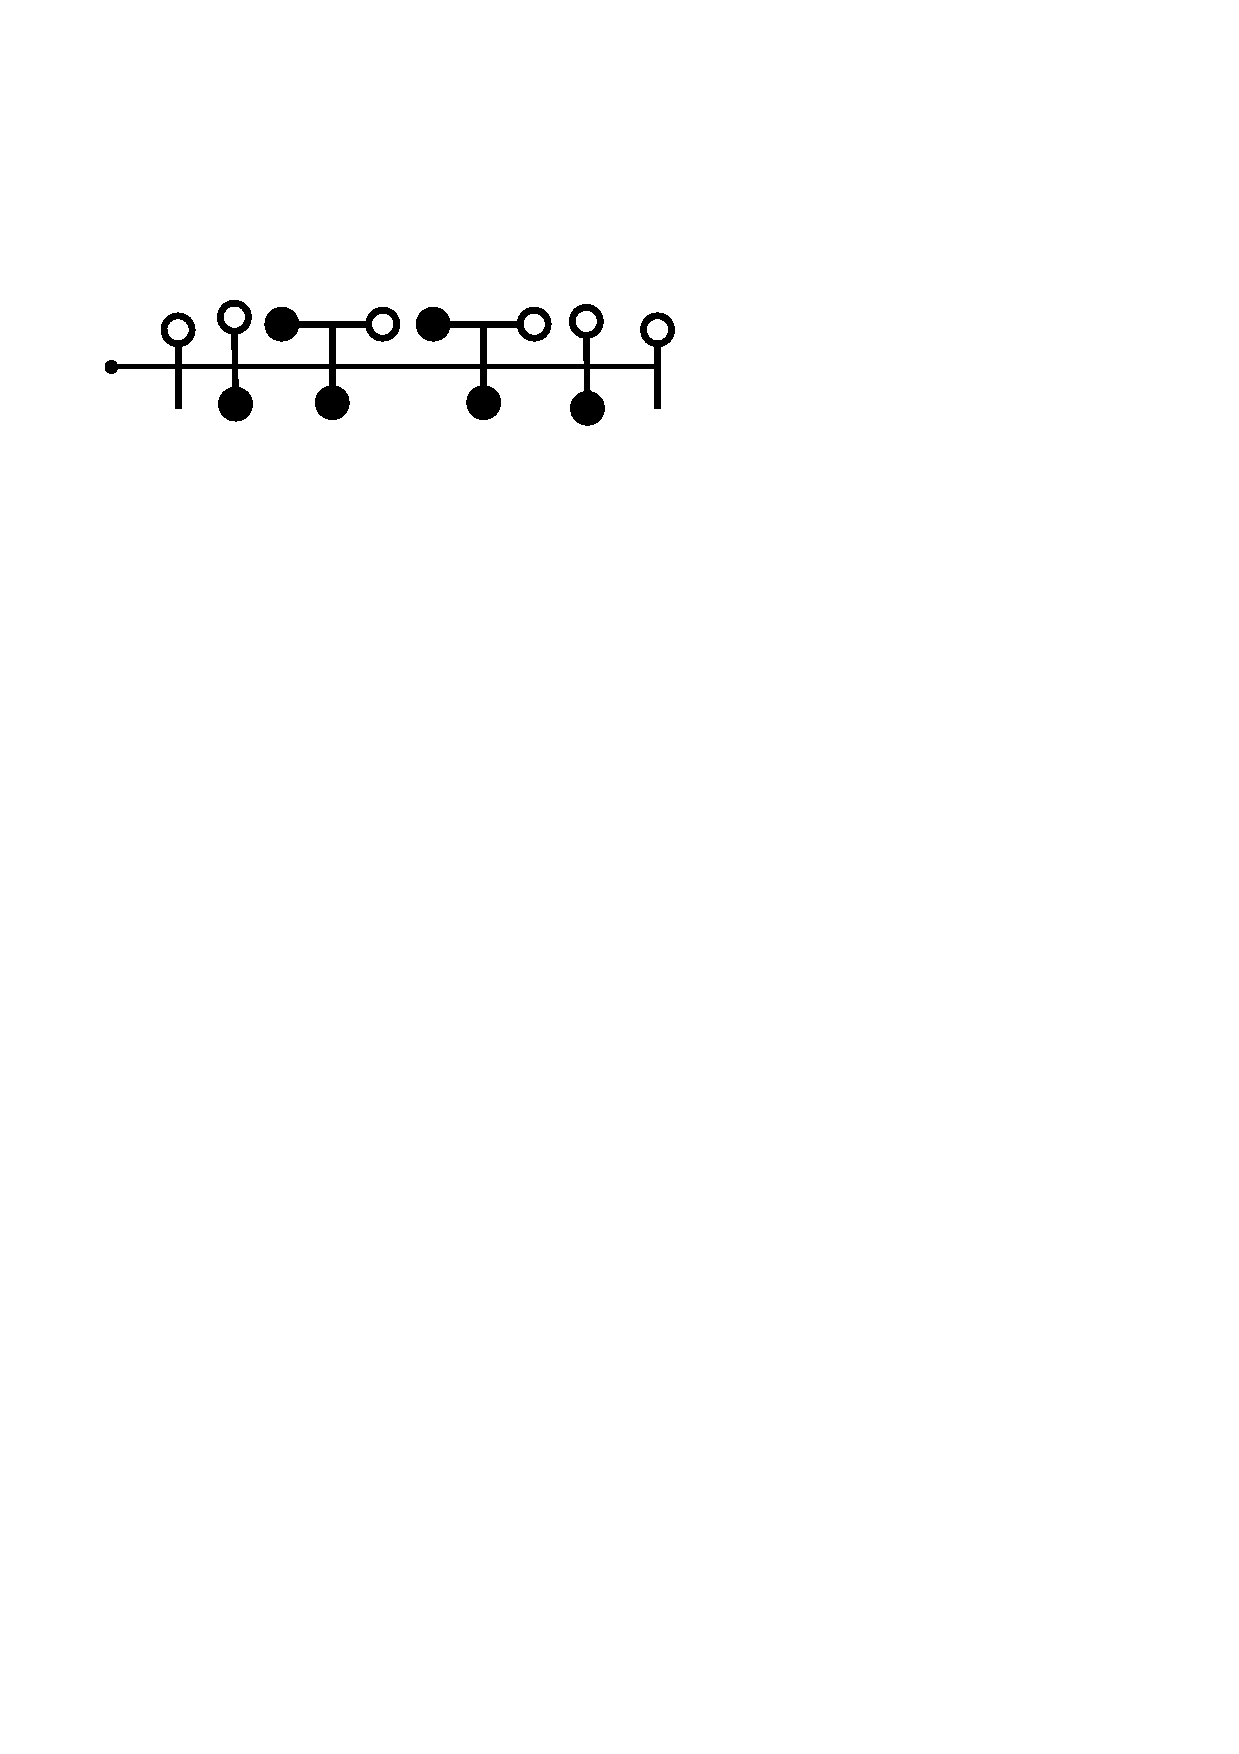
\includegraphics[trim=0cm 22cm 7cm 5cm, clip, width=0.9\textwidth,]{resources/pdfs/OZINCIPHER-APP4-PAL.pdf}\\
   \caption{The palindromic sequence $\Omega_{pal}$ transcribed into base-OZ.}
  \label{FIGOZPAL}
  \end{center}
\end{figure}

Now, notice something interesting here. In particular, if we compare the transcribed forms of $\Omega_{pal}$ and $\Omega_{3}$, we shall notice that even though the two sequences had some differences --- for example, $\Omega_{3}$ contains the ``0" symbol twice, including at the start, and yet, somewhat, because that STOP-codon is skipped during expression/transcription, so we note that the OZIN-expressions of the two sequences are somewhat similar --- they both share a similar prefix structure, that upon inspection of their genetic code sequences, can be attributed to the 3-gram subsequence ``123".

In fact, this later case is an interesting way to appreciate that even where two organisms, genes or proteins might exhibit significant differences in their appearance or even genetic code, and yet, upon close inspection, we might find some telling signs that they share some \textbf{common-traits}. In this case, we see that the palindromic $\Omega_{pal}$ looks somewhat like the otherwise different $\Omega_{3}$ --- at least in their prefix structures after transcription (and possibly beyond!)

\subsection{Genetic Code Sequences Interpreted as Modal Sequence Statistics}

Now that we have finished looking at how to express genetic code from its base/storage-form (equivalent to DNA) into its intermediate-form (equivalent to RNA), we can then consider the matter of how that intermediate code eventually gets \textbf{translated} into the final organism\footnote{We say ``final organism" here, because, much as in reality, genome expression might be more complex than merely translating genetic code from DNA into RNA and then final proteins and tissue, and yet, conceptually, that is all there is to it!}.

So, in further advancement our thought experiment concerning genome expression (modeled using hypothetical bio-automata), we shall again utilize the OZIN cipher introduced in \textbf{Section \ref{SECOZIN}}, but shall also introduce another formalism in the form of decoding position within a sequence (such as genetic code in this case), as information about how to express or process the associated symbols. This idea, of leveraging \textit{subtle instructions} embedded in genetic code but which might not be explicit as the actual nucleic acid combinations (such as amino-acid encoding-codons), can be justified when we consider that the genetic code processor (such as the ribosome in our major context --- see \textbf{Section \ref{SEC5}}), has a way of interpreting sequences not just by what they contain, but also based on the context within which they exist. For example, though generally the appearance of the RNA codon, \textbf{AAA} would cause the ribosome to synthesize the corresponding amino-acid Lysine (see \textbf{Table \ref{TAB1}}), and yet, if such a codon appears in a sequence where no earlier instruction compels the ribosome to START manufacturing a protein, the appearance of that codon shall be useless --- or rather, it shall be interpreted differently merely because of being in the wrong context. We saw this in \textbf{Section \ref{SEC05}}, and especially the Ribosome's protein-manufacturing process diagram (\textbf{Figure \ref{FIG3}}) as well as the State Machine (\textbf{Figure \ref{FIG4}}) help bring this out clearly. For example, if we modify the gene-program  in \textbf{Equation \ref{EQ6}} as such:


 \begin{equation}
\label{EQ6B}
\Theta_4^* = \langle \langle A, A, A \rangle, \langle A, U, G \rangle, \langle U, U, A \rangle, \langle U, A, G \rangle \rangle
\end{equation}\\


Then, where we would have expected the ribosome to manufacture protein whose structure includes the AAA/Lysine amino-acid, the result/effect of our modified sequence shall actually be different from what the original gene-program would have produced. In particular, since the START-codon, AUG (Methionine) appears after AAA, the effective protein to be synthesized would be as equivalent to just the program:

 \begin{equation}
\label{EQ6C}
\Theta_4^* = \langle \langle A, U, G \rangle, \langle U, U, A \rangle, \langle U, A, G \rangle \rangle
\end{equation}\\

Which would produce the protein with just \textbf{UUA}(Leucine) in it! So, position of symbols or terms within genetic code matters, and does encode some important gene or even genome expression information that we can't take for granted, thus the following suggested system for how to express post-RNA genetic code sequences.

\subsubsection{The Platonic Form Cipher and Positional-Sensitive Genetic Code Translation}

Just like we developed a system for how to map numbers (in base-10) to some non-trivial expressions that we equate to a kind of intermediate genetic code (the OZIN-encoded expressions), we shall similarly start by considering a way to map (still base-10) numbers to spatial-structures\footnote{Especially because, and essentially that, when compared to the code that expresses them, proteins and the organism taken as a whole, \textit{occupy more space} than does just the basic DNA code from which they are expressed.}.

So, with the exception of ``0'', which again is treated as an instruction to `skip' or `stop' within our genome expression system, we shall adopt the mapping from numbers to spatial-structures as depicted in \textbf{Figure \ref{FIGPLATOCIPHER}}.



\begin{center}
\fbox{\begin{minipage}{0.9\textwidth}
\large
\textbf{NOTE:}\\
 On \textbf{Why Place-Notation Expression Systems Matter} \\

As a further justification for why we chose to use a place-notation sensitive genetic code expression system in our conceptual genome expression thought experiment, consider that, just like with modern numbers --- of which the Arabic number system is considered one of the best since ancient times, the appearance of a symbol within an expression is interpreted not just by what it quantifies, but also by where in the expression it is placed. 

For good measure, a few enlightening quotes from the priceless work on the evolution of number systems since ancient times, by Raymond S. Nickerson, shall help cement this:

\begin{quotation}
\noindent \texttt{Aristotle attached considerable significance to the fact that human beings can count: it is this ability, he claimed, that demonstrates our rationality.}\\\\

\noindent \texttt{As Brainerd (1973) has pointed out, in most Western nations today we expect students, by the time they reach their early teens, to be much more competent with numbers than was an educated adult Greek or Roman of 2,000 years ago. This fact arises in no small measure from the elegance and power of the scheme that we now use to represent numbers.}\\\\


\noindent \texttt{In short, a price of the increased abstractness of the Arabic system is an obscuring of some of the key principles on which numbers are based. To an ancient Egyptian, the fact that 3+4=7 was apparent from the relationship between the Egyptian number representing 7 and those representing 3 and 4. There is no hint of such a relationship, however, when this equation is expressed in Arabic notation. The price has been worth the paying, however.}\\\\


\noindent \texttt{If you invented a unique symbol to represent each of the possible quantities of stones (including the case of no stones) up to that of your standard and decided to use the position of that symbol to indicate the pile to which it refers, you would have what we refer to today as a place-notation system for representing numbers.}\\\\

\noindent \texttt{The relative ease with which one can count or compute depends to no small degree on the characteristics of the system that is used to represent number concepts.}\\

\hspace*{\fill} ---\textbf{Raymond S. Nickerson}, \textit{Counting, Computing, and the Representation of Numbers}, 1988\cite{nickerson1988counting}
\end{quotation}

And finally, it shall be worth noting that this notion also underlies the present author's use of the \textbf{Position-Index measure} ($I(\omega_i, \Theta)$), first formalized in the Base-36 paper\cite{base36paper}, and which, among many important applications it has, is its use in generalizing the computation of decimal values of arbitrary number expressions in any base, its use in transformatics to express sequence summaries using modal sequences\cite{transformatics}, etc.

\end{minipage}}
\\
\end{center}


\section{Conclusion}
\label{CONC}

In this paper, we have advanced our knowledge concerning...

\begin{appendices}

\chapter{Origins of the OZIN Cipher}
\label{APPOZIN}

\begin{figure}[H]
  \begin{center}
  %\includegraphics[trim=2cm 8cm 2cm 8cm, clip, width=0.9\textwidth,]{resources/pdfs/ProteinSynthesisStateMachine.pdf}\\
   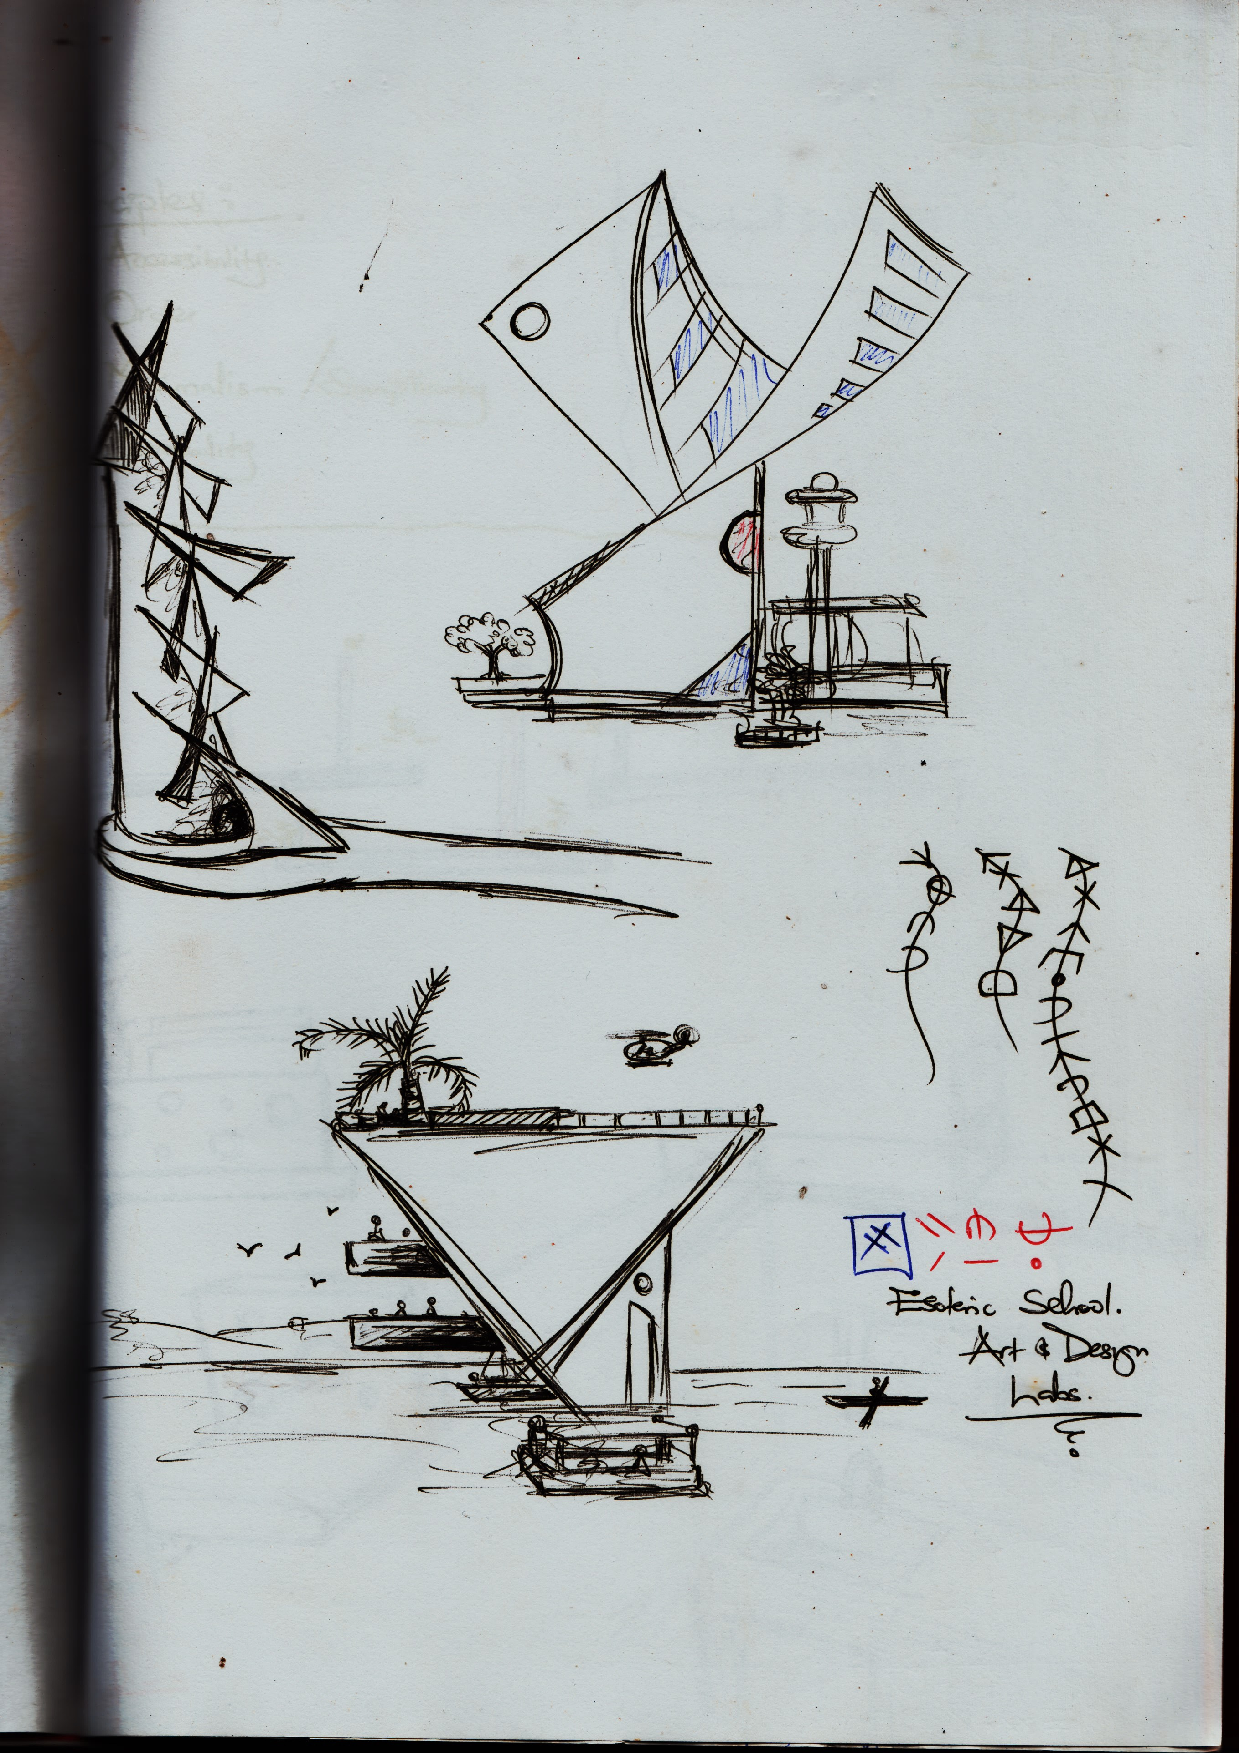
\includegraphics[trim=0cm 4cm 0cm 2.8cm, clip, width=0.9\textwidth,]{resources/pdfs/ozin_gene_expressions.pdf}\\
   \caption{An excerpt from architectural design notes by the author from early days of his home-based research laboratory. In this note, we also get to see an idea similar to how gene expressions are actually a chain of glyphs that, as in our Ozin-expressions, are depicted as structures chained to each other along a \textit{backbone structure} symbolically depicted as a line (curved lines in this case). Copyrights due to author and Nuchwezi Research Labs.}
  \label{FIGCODEOZINART}
  \end{center}
\end{figure}


For some, the \textbf{Ozin Cipher} (see \textbf{Section \ref{SECOZIN}}) might not seem that important or useful, but, perhaps because not everyone can immediately appreciate the fact that cryptography is such a dear part of expression in nature, that whoever is the Architect of Life, has applied it throughout nature in many creative ways --- camouflage in reptiles and viruses, the occult languages of birds, etc. And these phenomena have indeed inspired many observant minds throughout the ages, to pick a leaf from nature and apply these ideas (in \textit{alternative information expression}) in everything including mathematics, philosophy and yes... \textit{magick}! Talking of which, for those interested in getting a deeper idea concerning how such a beautiful numeric symbol system --- an alternative to the commonplace Arabic Numerals, came to be, one useful resource is the \textbf{CODE OGF}\cite{lutalo_2025_ogf}.

\begin{figure}[H]
  \begin{center}
  %\includegraphics[trim=2cm 8cm 2cm 8cm, clip, width=0.9\textwidth,]{resources/pdfs/ProteinSynthesisStateMachine.pdf}\\
   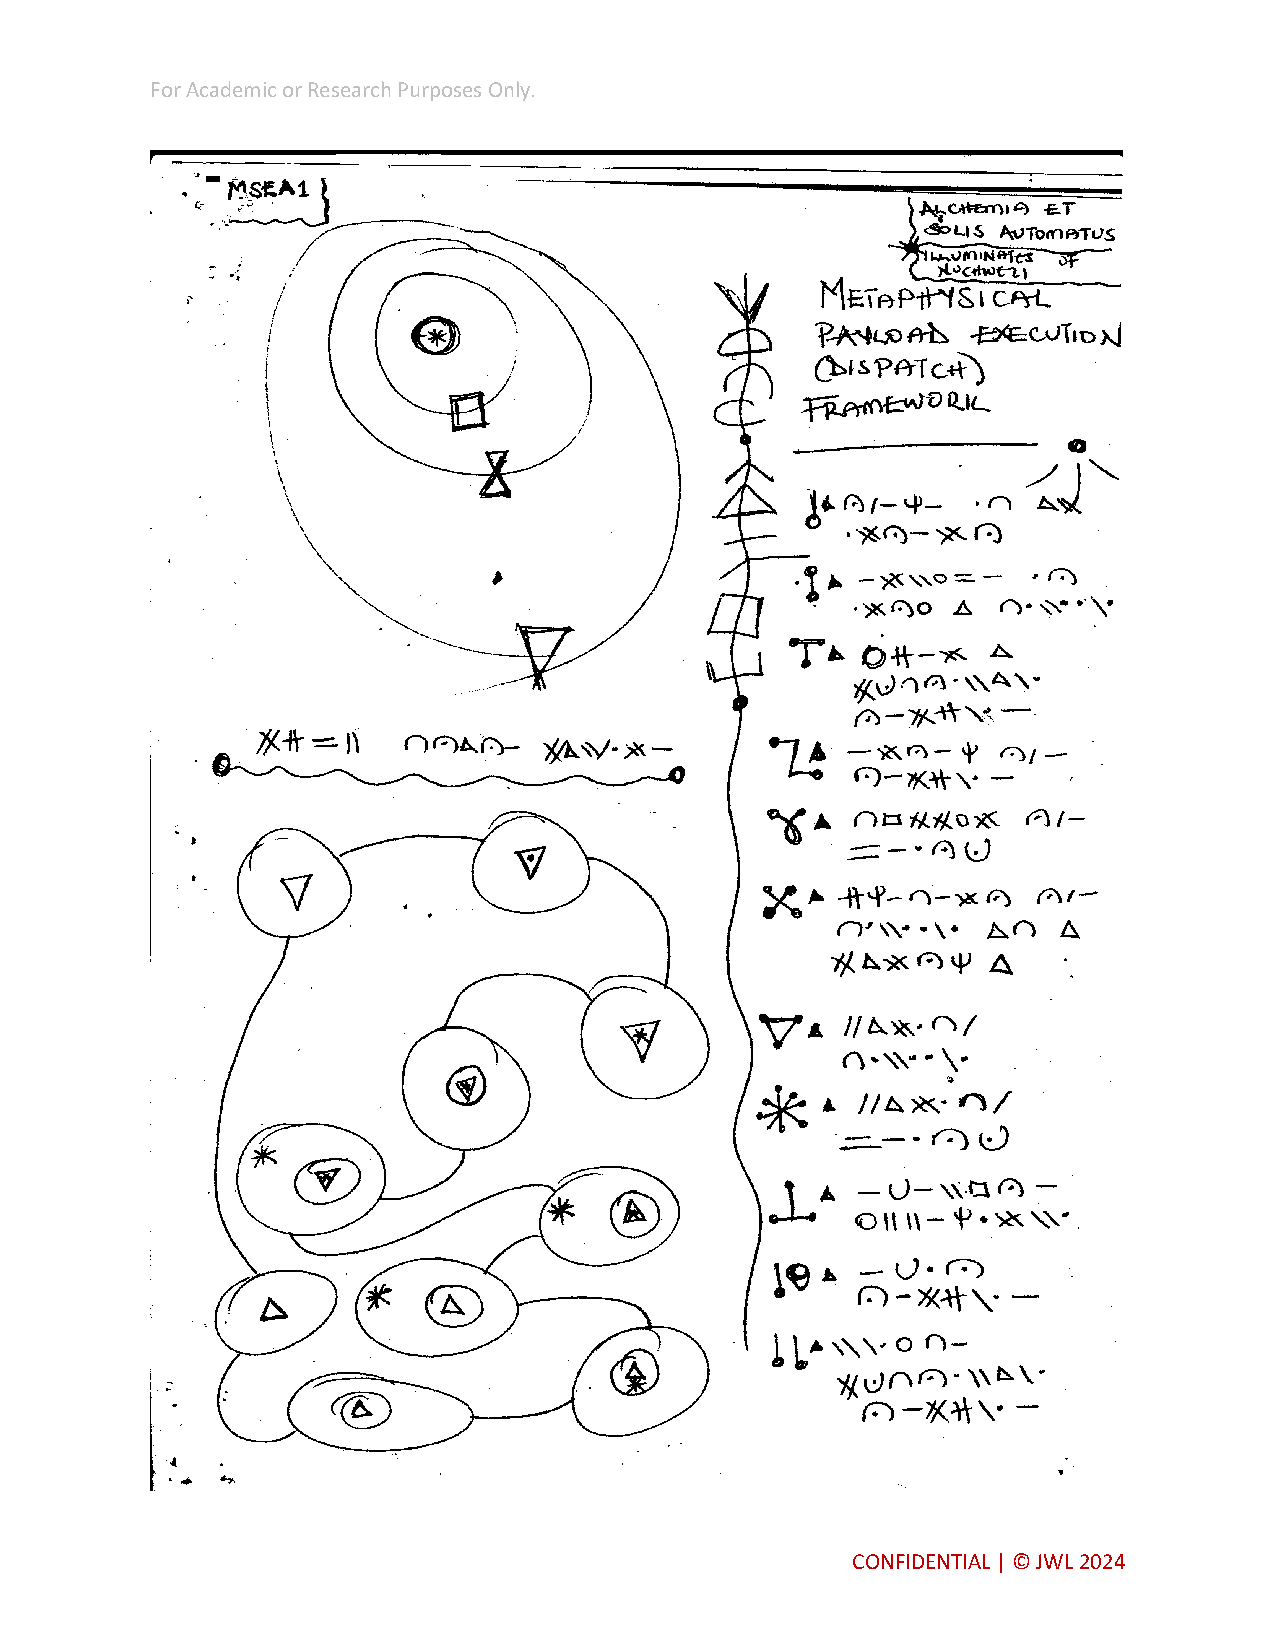
\includegraphics[trim=0cm 2cm 0cm 0cm, clip, width=0.9\textwidth,]{resources/pdfs/ozin.pdf}\\
   \caption{The OZIN Cipher in use. An excerpt from the Church of Dance Eternal OGF}
  \label{FIGCODEOZIN}
  \end{center}
\end{figure}

\textbf{Figure \ref{FIGCODEOZIN}} is just an excerpt from that manuscript, perhaps not so clear because the original manuscript is handwritten, and this is just a scanned version. But hopefully it drives the point home. Also, as seen from that excerpt as well as a closely related excerpt --- see \textbf{Figure \ref{FIGCODEOZINNOTES}}, just like we might replace numbers with alternative symbols, we also see the Latin Alphabet replaced by an ``alien-looking" hand, and this might definitely have its place in transformations of $\psi_{az}$ sequences or their expression in other ways! 


\begin{figure}[H]
  \begin{center}
  %\includegraphics[trim=2cm 8cm 2cm 8cm, clip, width=0.9\textwidth,]{resources/pdfs/ProteinSynthesisStateMachine.pdf}\\
   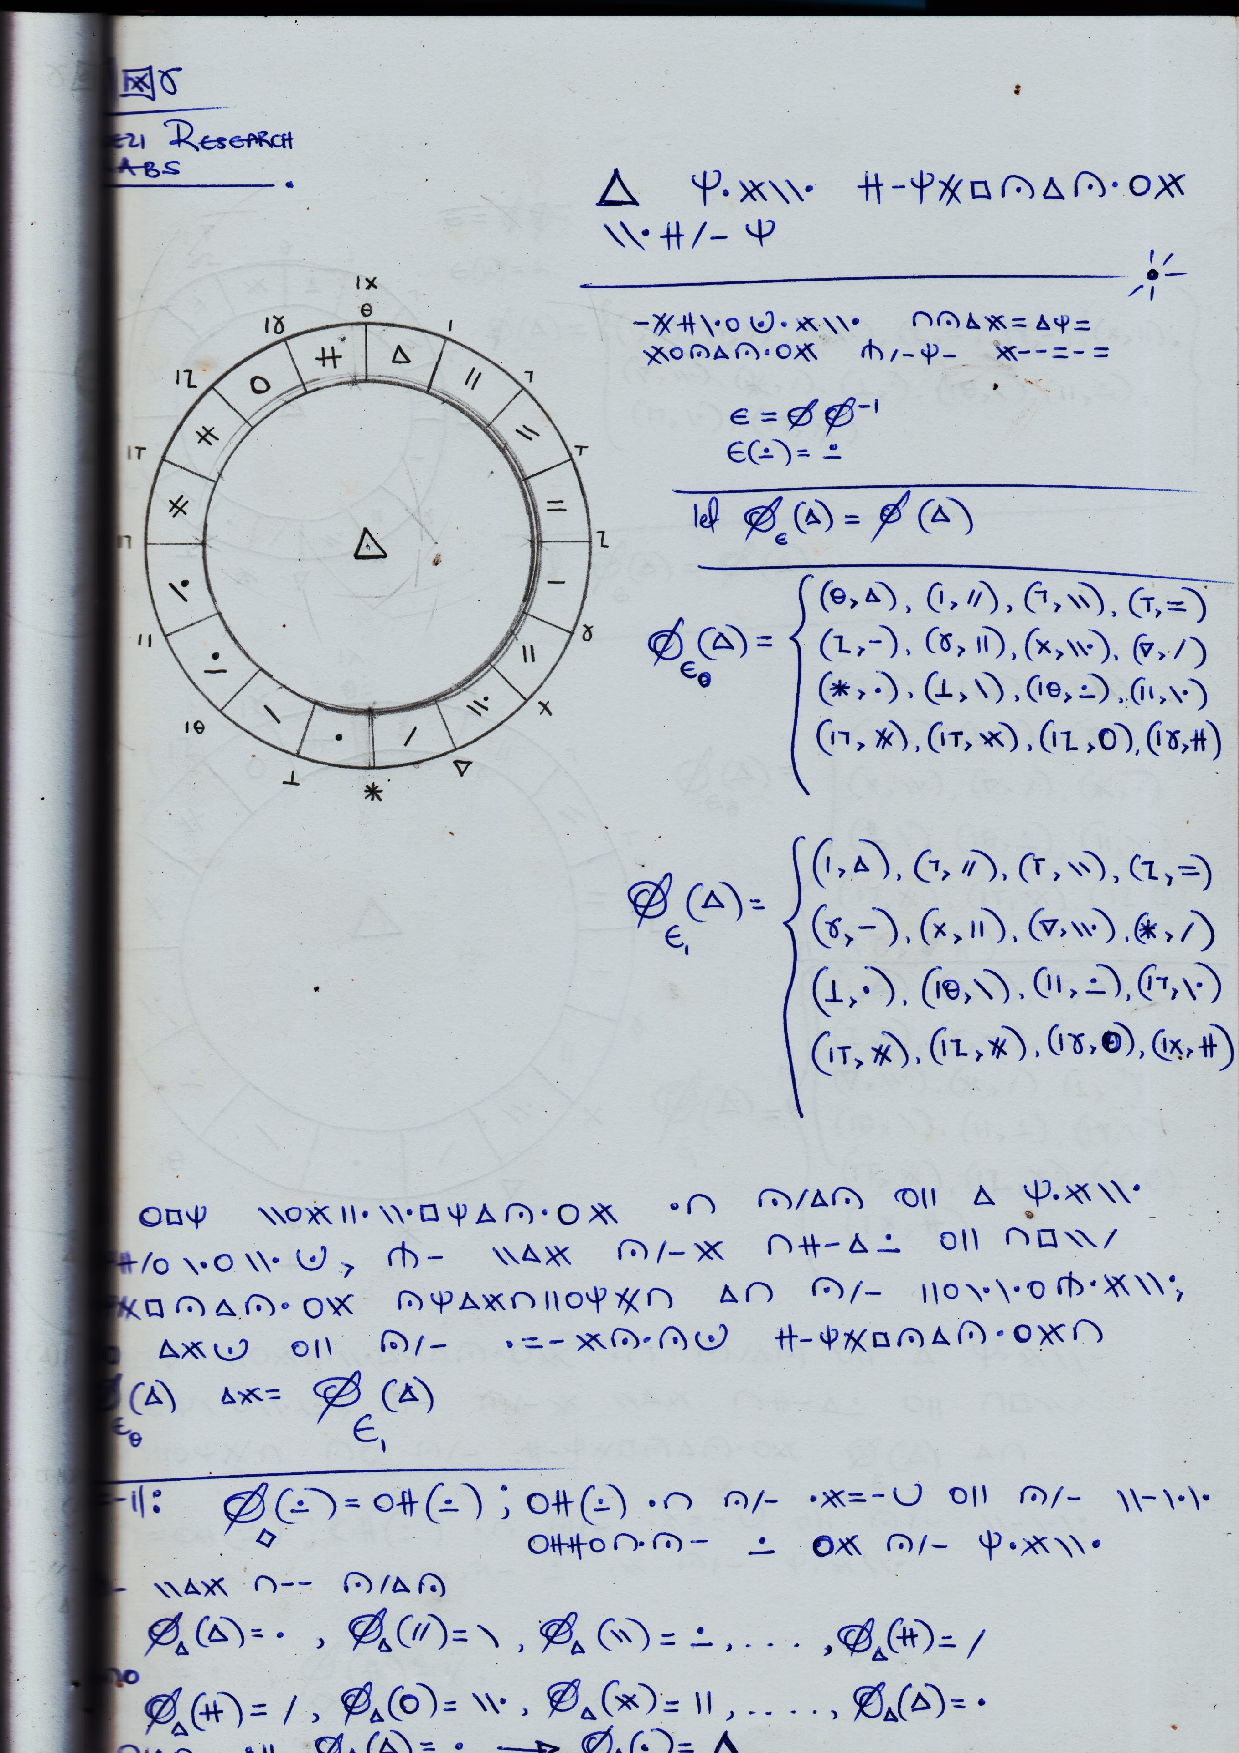
\includegraphics[ width=0.9\textwidth,]{resources/pdfs/ozin_applied.pdf}\\
   \caption{The OZIN Cipher in use. An excerpt from author's research notes (circa 2019) on developing a cryptographic system leveraging a dial mechanism. Copyrights due to author and Nuchwezi Research Labs.}
  \label{FIGCODEOZINNOTES}
  \end{center}
\end{figure}


\end{appendices}

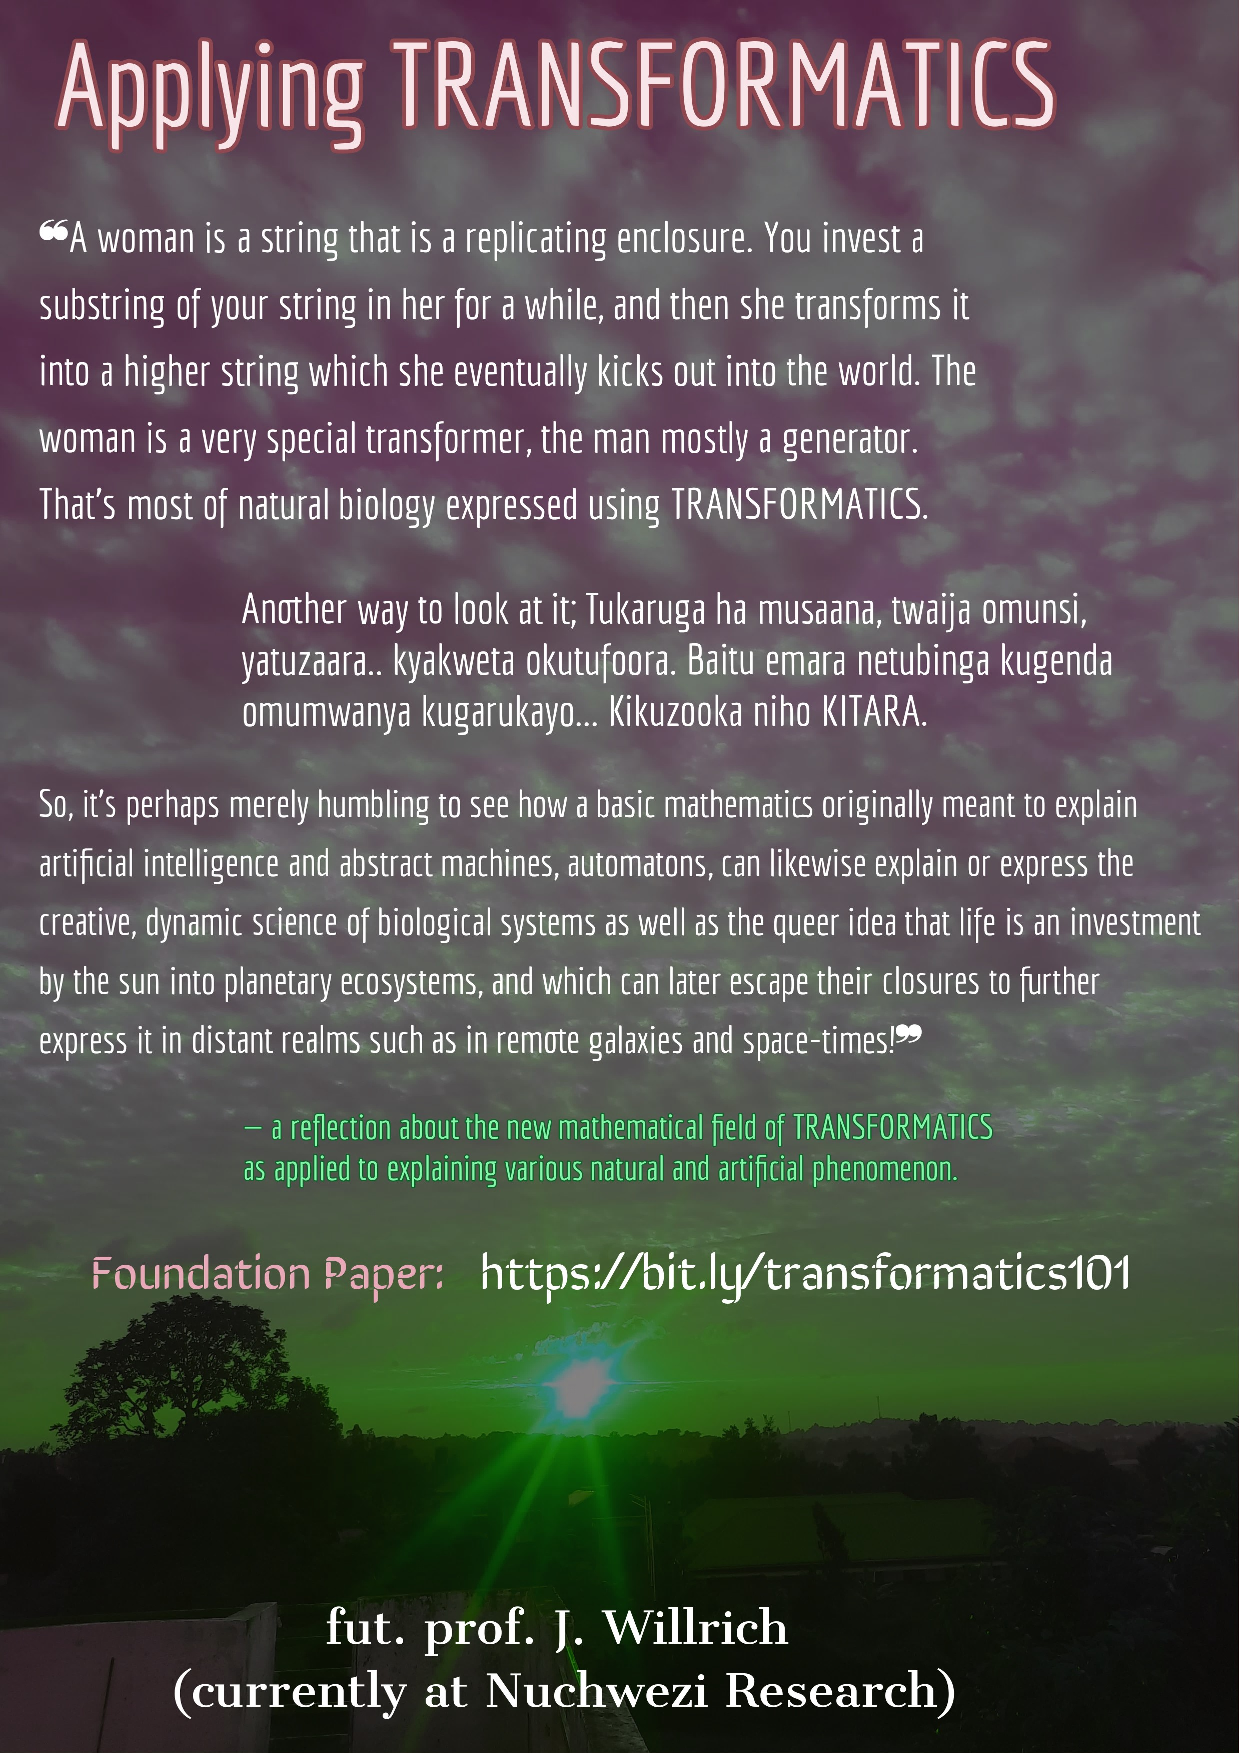
\includepdf[pages=1]{resources/pdfs/note_cover.pdf}

\bibliographystyle{unsrt}
\bibliography{references}

\comment{
\vspace{5cm}
\fbox{
\begin{minipage}{0.9\textwidth}
\textbf{TO CITE:}\\

Lutalo, Joseph Willrich (2025). \textbf{The Theory of Sequence Transformers \& their Statistics:} \textit{The 3 Information Sequence Transformer Families (Anagrammatizers, Protractors, Compressors) and 4 New and Relevant Statistical Measures Applicable to Them: Anagram Distance, Modal Sequence Statistic, Transformation Compression Ratio and Piecemeal Compression Ratio.} figshare. Online Resource. \url{https://doi.org/10.6084/m9.figshare.29505824.v3}

\end{minipage}}
\\
}


% insert [back] cover --- could just be a PNG or PDF
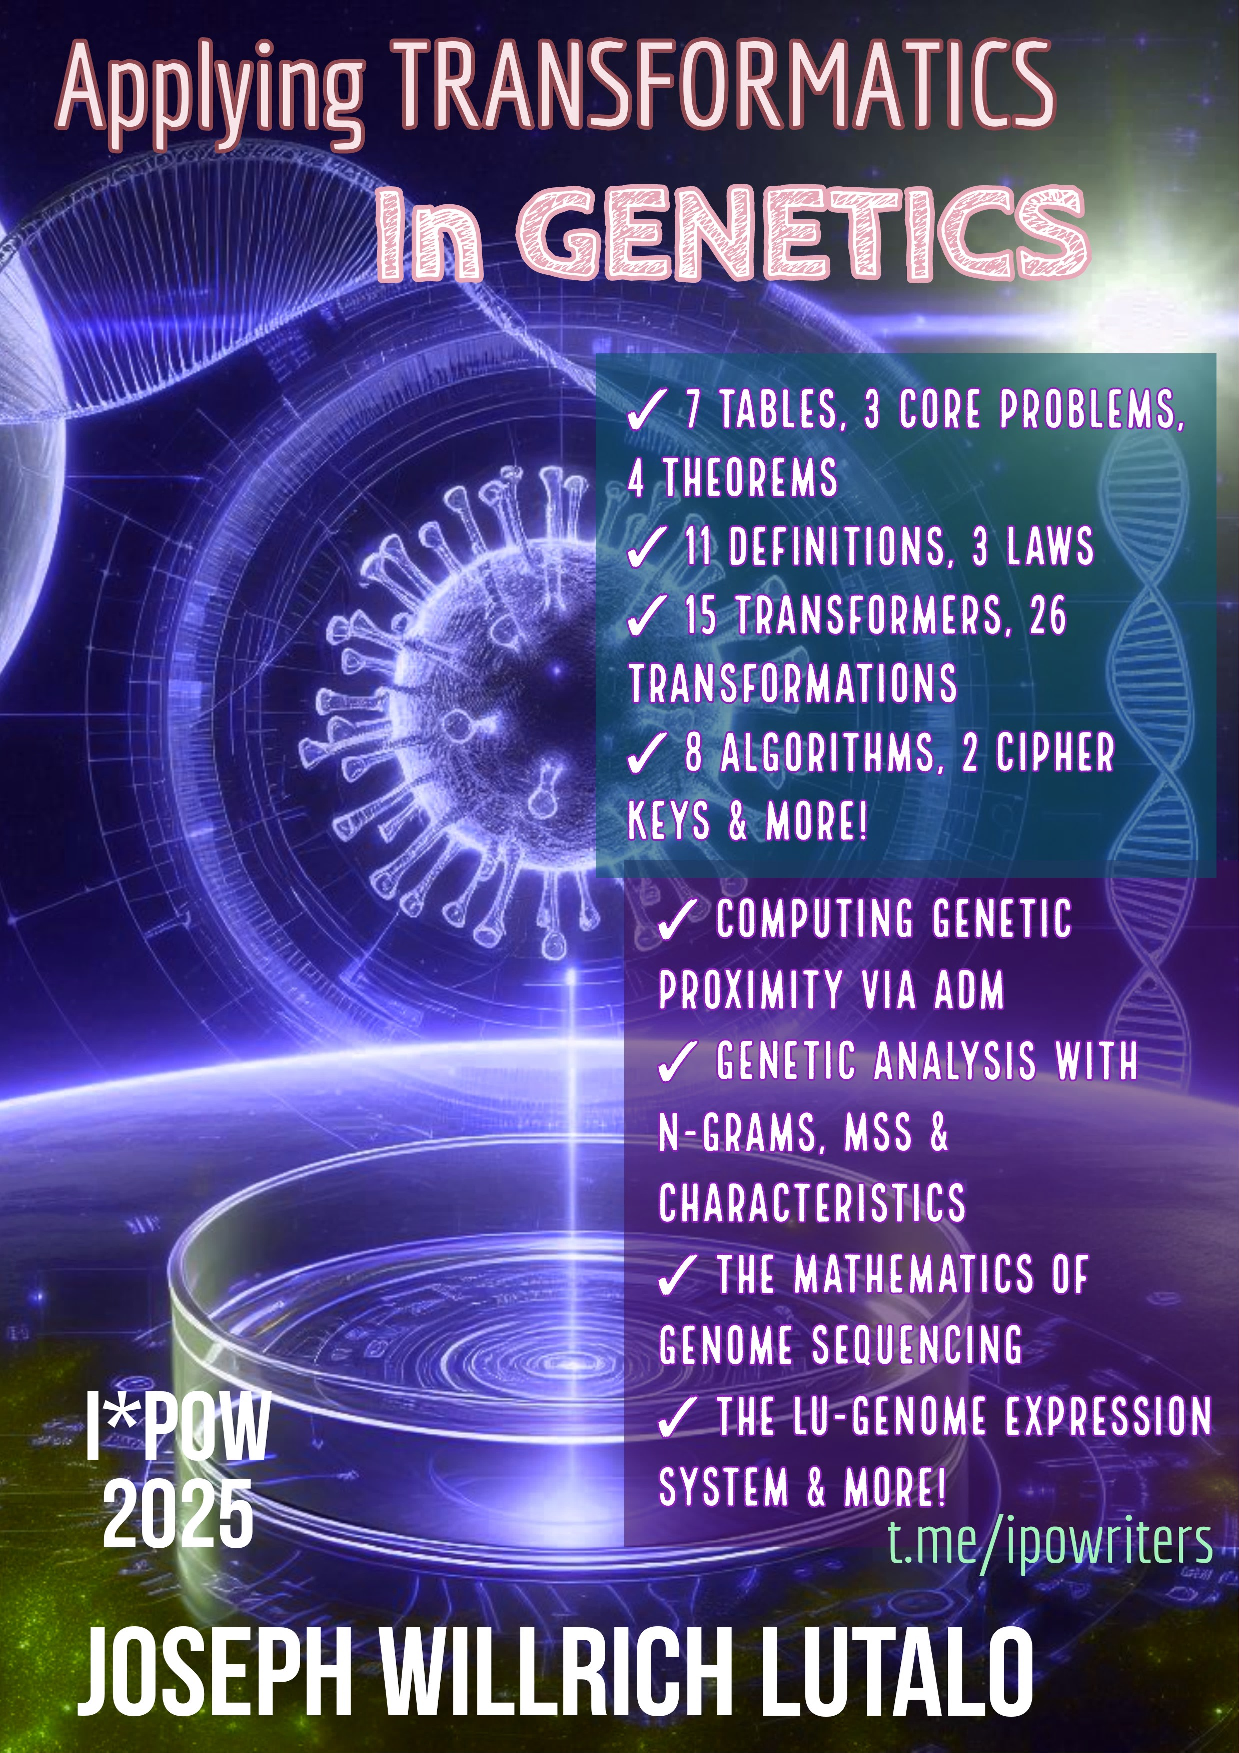
\includepdf[pages=1]{resources/pdfs/back_cover.pdf}

\end{document}
